%%%%%%%%%%%%%%%%%%%%%%%%%%%%%%%%%%%%%%%%%%%%%%%%%%%%%%%%%%%%%%%%%%%%%%%%%%%%%%%
%                       CARREGA DE LA CLASSE DE DOCUMENT                      %
%                                                                             %
% Les opcions admissibles son:                                                %
%      12pt / 11pt            (cos dels tipus de lletra; no feu servir 10pt)  %
%                                                                             %
% catalan/spanish/english     (llengua principal del treball)                 %
%                                                                             % 
% french/italian/german...    (si necessiteu fer servir alguna altra llengua) %
%                                                                             %
% listoffigures               (El document inclou un Index de figures)        %
% listoftables                (El document inclou un Index de taules)         %
% listofquadres               (El document inclou un Index de quadres)        %
% listofalgorithms            (El document inclou un Index d'algorismes)      %
%                                                                             %
%%%%%%%%%%%%%%%%%%%%%%%%%%%%%%%%%%%%%%%%%%%%%%%%%%%%%%%%%%%%%%%%%%%%%%%%%%%%%%%

\documentclass[11pt,spanish,listoffigures]{tfgetsinf}

%%%%%%%%%%%%%%%%%%%%%%%%%%%%%%%%%%%%%%%%%%%%%%%%%%%%%%%%%%%%%%%%%%%%%%%%%%%%%%%
%                     CODIFICACIO DEL FITXER FONT                             %
%                                                                             %
%    windows fa servir normalment 'ansinew'                                   %
%    amb linux es possible que siga 'latin1' o 'latin9'                       %
%    Pero el mes recomanable es fer servir utf8 (unicode 8)                   %
%                                          (si el vostre editor ho permet)    % 
%%%%%%%%%%%%%%%%%%%%%%%%%%%%%%%%%%%%%%%%%%%%%%%%%%%%%%%%%%%%%%%%%%%%%%%%%%%%%%%

\usepackage[utf8]{inputenc} 
\usepackage{multirow}
\usepackage{babel}

\usepackage[square,sort,comma,numbers]{natbib}
\bibliographystyle{miBST}

\graphicspath{ {Imagenes/} }

%%%%%%%%%%%%%%%%%%%%%%%%%%%%%%%%%%%%%%%%%%%%%%%%%%%%%%%%%%%%%%%%%%%%%%%%%%%%%%%
%                        ALTRES PAQUETS I DEFINICIONS                         %
%                                                                             %
% Carregueu aci els paquets que necessiteu i declareu les comandes i entorns  %
%                                          (aquesta seccio pot ser buida)     %
%%%%%%%%%%%%%%%%%%%%%%%%%%%%%%%%%%%%%%%%%%%%%%%%%%%%%%%%%%%%%%%%%%%%%%%%%%%%%%%

\usepackage{hyperref}
\hypersetup{colorlinks,linkcolor={black},citecolor={black},urlcolor={blue}} 

\usepackage{booktabs}
\newcommand{\tabitem}{~~\llap{\textbullet}~~}

%%%%%%%%%%%%%%%%%%%%%%%%%%%%%%%%%%%%%%%%%%%%%%%%%%%%%%%%%%%%%%%%%%%%%%%%%%%%%%%
%                        DADES DEL TREBALL                                    %
%                                                                             %
% titol, alumne, tutor i curs academic                                        %
%%%%%%%%%%%%%%%%%%%%%%%%%%%%%%%%%%%%%%%%%%%%%%%%%%%%%%%%%%%%%%%%%%%%%%%%%%%%%%%

\title{ Desarrollo de software basado en microservicios: un caso de estudio para evaluar sus ventajas e inconvenientes }
\author{Víctor Alberto Iranzo Jiménez}
\tutor{Patricio Orlando Letelier Torres}
\curs{2017-2018}

%%%%%%%%%%%%%%%%%%%%%%%%%%%%%%%%%%%%%%%%%%%%%%%%%%%%%%%%%%%%%%%%%%%%%%%%%%%%%%%
%                     PARAULES CLAU/PALABRAS CLAVE/KEY WORDS                  %
%                                                                             %
% Independentment de la llengua del treball, s'hi han d'incloure              %
% les paraules clau i el resum en els tres idiomes                            %
%%%%%%%%%%%%%%%%%%%%%%%%%%%%%%%%%%%%%%%%%%%%%%%%%%%%%%%%%%%%%%%%%%%%%%%%%%%%%%%

\keywords{Microservices, Arquitectura de software, } % Paraules clau 
         {Microservicios, Arquitectura de software, Proceso de desarrollo de software, Docker, Kubernetes, Microsoft Azure}              % Palabras clave
         {Microservices, Software Architecture, Software Development Process, Docker, Kubernetes, Microsoft Azure}        % Key words

%%%%%%%%%%%%%%%%%%%%%%%%%%%%%%%%%%%%%%%%%%%%%%%%%%%%%%%%%%%%%%%%%%%%%%%%%%%%%%%
%                              INICI DEL DOCUMENT                             %
%%%%%%%%%%%%%%%%%%%%%%%%%%%%%%%%%%%%%%%%%%%%%%%%%%%%%%%%%%%%%%%%%%%%%%%%%%%%%%%

\begin{document}

%%%%%%%%%%%%%%%%%%%%%%%%%%%%%%%%%%%%%%%%%%%%%%%%%%%%%%%%%%%%%%%%%%%%%%%%%%%%%%%
%              RESUMS DEL TFG EN VALENCIA, CASTELLA I ANGLES                  %
%%%%%%%%%%%%%%%%%%%%%%%%%%%%%%%%%%%%%%%%%%%%%%%%%%%%%%%%%%%%%%%%%%%%%%%%%%%%%%%

\begin{abstract}[spanish]

Las arquitecturas basadas en microservicios son una tendencia actual en la cual una aplicación software se compone de servicios pequeños y autónomos que cooperan entre ellos para ofrecer diversas funcionalidades.  El objetivo de este trabajo es validar las ventajas e inconvenientes de una arquitectura basada en microservicios frente a una arquitectura tradicional o monolítica mediante la evaluación de un caso de estudio. Con este propósito, se hará una revisión de la influencia de los microservicios en el proceso de desarrollo de software y se repasarán las principales herramientas asociadas a su despliegue.

El caso de estudio consistirá en el diseño e implementación de una aplicación móvil para el comercio electrónico (e-shop). La parte servidora se implementará dos veces siguiendo arquitecturas diferentes: una basada en microservicios y otra monolítica. Para el despliegue del sistema se emplearán contenedores Docker orquestados por la herramienta Kubernetes, dentro de la plataforma Microsoft Azure.

Finalmente, ambas soluciones se compararán frente a diferentes requisitos no funcionales, como la disponibilidad o la tolerancia a fallos, y distintas situaciones de mantenimiento. 

\end{abstract}

\begin{abstract}[english]

Architectures based on microservices are a latest trend where software application consists of small and autonomous services that cooperate between themselves offering several functionalities. The aim of this work is to validate advantages and drawbacks from an architecture based on microservices compared to a traditional or monolithic one with a study case evaluation. With this purpose, influence of microservices on software development process was reviewed likewise inspection of the main tools associated with its deployment.

The study case consisted of the design and implementation of a mobile application for electronic commerce (e-shop) purposes. The server-side was twice implemented following different architectures: one microservices-based and a monolithic one. The system deployment employed Docker containers orchestrated by Kubernetes tool within Microsoft Azure platform.

Finally, both solutions were compared in front of diverse non-functional requirements, such us availability or fault tolerance, and several maintenance situations.

\end{abstract}

%%%%%%%%%%%%%%%%%%%%%%%%%%%%%%%%%%%%%%%%%%%%%%%%%%%%%%%%%%%%%%%%%%%%%%%%%%%%%%%
%                              CONTINGUT DEL TREBALL                          %
%%%%%%%%%%%%%%%%%%%%%%%%%%%%%%%%%%%%%%%%%%%%%%%%%%%%%%%%%%%%%%%%%%%%%%%%%%%%%%%

\mainmatter

%%%%%%%%%%%%%%%%%%%%%%%%%%%%%%%%%%%%%%%%%%%%%%%%%%%%%%%%%%%%%%%%%%%%%%%%%%%%%%%
%                                  INTRODUCCION                                %
%%%%%%%%%%%%%%%%%%%%%%%%%%%%%%%%%%%%%%%%%%%%%%%%%%%%%%%%%%%%%%%%%%%%%%%%%%%%%%%

\chapter{Introducci\'on}

\section{Motivaci\'on}

% Referencia a The Clean Architecture.
En la actualidad, no es necesario un alto grado de conocimientos en ingeniería del software para desarrollar una aplicación o sistema. Personas que no tienen estudios relacionados con la informática pueden producir código que, sin ser limpio y elegante, funciona. Sin embargo, desarrollar sistemas de calidad requiere de grandes conocimientos, pero minimiza los costes y aumenta la productividad de una organización. Se debe poner el foco en emplear una arquitectura de software que se adapte a las necesidades del negocio; de lo contrario, el futuro mantenimiento será más costoso y repercutirá en la confianza de los clientes y en la moral del equipo \cite{Martin2017}.

El presente trabajo se ha desarrollado en el contexto de una colaboración con una PYME dedicada al desarrollo software. Esta empresa desarrolla un ERP para el sector socio-sanitario a la vez que apuesta por el uso de las tecnologías más punteras, como es el uso de microservicios. El autor de esta memoria ha colaborado en este espacio desarrollando algunos microservicios y herramientas que facilitan su construcción a través de la generación automática de código. La realización de este trabajo tiene como motivación profundizar en el conocimiento de las tecnologías asociadas a los microservicios, más allá de las utilizadas por esta organización.

Si bien ya existe bastante bibliografía destacando los beneficios de este tipo de arquitecturas, los ejemplos que se ilustran son muy básicos. Por este motivo, este trabajo pretende conocer de primera mano la realidad de este tipo de arquitecturas mediante la realización de un caso de estudio de tamaño superior a los presentados en la literatura. Para ello, se desarrollará una aplicación de forma integral empleando tecnologías lo más cercanas posibles a las que se usarían en el desarrollo profesional de un producto software.

%%%%%%%%%%%%%%%%%%%%%%%%%%%
% SALTO DE PAGINA
%%%%%%%%%%%%%%%%%%%%%%%%%%%
\newpage

\section{Objetivos}
%TODO Revisar.

El objetivo de este proyecto es validar con un caso de estudio las ventajas e inconvenientes de una arquitectura basada en microservicios frente a una arquitectura monolítica. Concretamente,los objetivos específicos son:

\begin{itemize}

\item Desarrollar una misma aplicación para la venta de productos y la gestión de pedidos siguiendo dos arquitecturas diferentes: una basada en microservicios y otra monolítica.

\item Comparar el proceso de desarrollo de ambos sistemas a lo largo del ciclo de vida del software.

\item Evaluar cómo se pueden llevar a cabo diferentes modificaciones durante el mantenimiento de ambas aplicaciones una vez se ha finalizado su implementación.

\item Examinar ambas arquitecturas respecto a los siguientes requisitos no funcionales: disponibilidad, tolerancia a fallos, utilización de recursos y capacidad para ser reemplazado.

\end{itemize}

\section{Estructura de la memoria}

A continuación, se presenta la estructura de la memoria:

El capítulo 1 introduce la memoria a través de la motivación del trabajo y los objetivos a cumplir.

En el capítulo 2 se presenta una definición para el término microservicio y se describe su influencia en el proceso de desarrollo a lo largo del ciclo de vida del software.

El capítulo 3 presentará brevemente el estado del arte asociado a la tecnología de los microservicios, explicando brevemente algunas de las herramientas más empleadas.

En el capítulo 4 se analiza la aplicación a desarrollar mediante su especificación   empleando casos de uso y un modelo de dominio.

El capítulo 5 contiene el proceso de desarrollo y la organización del trabajo que se seguirá durante la implementación de las dos soluciones propuestas.

El capítulo 6 explica el diseño e implementación del sistema siguiendo una arquitectura monolítica. En este capítulo se repasan las principales herramientas utilizadas y los aspectos más relevantes de la construcción del sistema.

El capítulo 7 se centra en los mismos aspectos que el capítulo anterior pero para una arquitectura basada en microservicios. El foco en este capítulo está puesto en el diseño del sistema y las diferencias entre ambas soluciones.

En el capítulo 8 se realiza una comparación de ambas soluciones respecto a diferentes requisitos no funcionales  y se evalúa como afrontaría cada solución diferentes situaciones de mantenimiento.

El último capítulo presenta las conclusiones del trabajo respecto a los objetivos planteados inicialmente.

Adicionalmente, al final de la memoria se adjuntan un conjunto de apéndices. En ellos  se incluye un modelo de la aplicación desarrollada y se detallan los pasos para el despliegue de la solución basada en microservicios en un entorno de producción.

%%%%%%%%%%%%%%%%%%%%%%%%%%%%%%%%%%%%%%%%%%%%%%%%%%%%%%%%%%%%%%%%%%%%%%%%%%%%%%%
%              Los microservicios en el proceso de desarrollo
%
%%%%%%%%%%%%%%%%%%%%%%%%%%%%%%%%%%%%%%%%%%%%%%%%%%%%%%%%%%%%%%%%%%%%%%%%%%%%%%%

\chapter{Los microservicios en el proceso de desarrollo}

\section{¿Qué son los microservicios?}

Según Newman, \cite{Newman2015a} los microservicios son servicios pequeños y autónomos que trabajan conjuntamente. Podemos desglosar esta definición así:

\begin{itemize}
%TODO Sustituir referencia a Wikipedia.

\item Un \textbf{servicio} es un conjunto de funcionalidades que se expone a los clientes para que las empleen con diferentes propósitos \cite{Wikipedia}. La programación orientada a servicios es un paradigma que se aplica en las arquitecturas orientadas a servicios (SOA) \cite{Arsanjani2009a}. El objetivo principal de SOA es desarrollar servicios que aporten valor al negocio y se adapten a los cambios en las necesidades de los clientes, de forma ágil y con el menor coste posible. Las arquitecturas orientadas a servicios no están asociadas a ninguna tecnología específica. En líneas generales, dividen un sistema en componentes que cambian por el mismo motivo y promueven la flexibilidad y los servicios compartidos frente a implementaciones específicas y óptimas. Son muchos los beneficios de estas arquitecturas, sin embargo existe una falta de consenso sobre cómo debe llevarse a cabo este tipo de arquitecturas en aspectos como los protocolos de comunicación a emplear o la granularidad de los servicios. Los microservicios pueden entenderse como una aproximación específica de las arquitecturas SOA. \footnote{ NOTA: A partir de este punto, se emplearán los términos servicio y microservicio como sinónimos para hacer más ligera la lectura.}

\item Diseñar microservicios con el menor \textbf{tamaño} posible no debe ser el foco principal. En todo momento han de cumplirse los principios de cohesión y coherencia: el código relacionado debe agruparse conjuntamente porque será modificado por el mismo motivo. \cite{Newman2015a}

\item  Los servicios han de ser lo menos acoplados posibles para garantizar la \textbf{autonomía} de cada uno. Cada microservicio es una entidad separada: cambian de forma independiente al resto y al hacerlo sus consumidores no necesiten ser modificados, a menos que se modifique el contrato entre ambas partes. Para lograrlo, lo más habitual es que cada servicio exponga una interfaz (API) y todas las comunicaciones se realicen mediante llamadas a través de la red. \cite{Newman2015a, Hunter2017}

\end{itemize}

Otra definición interesante es la que aportan Lewis y Fowler \cite{Lewis2014}. Según ellos, los microservicios son una aproximación para desarrollar una aplicación compuesta por pequeños servicios, cada uno ejecutándose en su propio proceso y comunicando a través de mecanismos ligeros. Estos servicios se construyen alrededor de las capacidades de negocio y se despliegan de forma independiente. Cada funcionalidad se encapsula en un servicio que puede escalar de forma diferente de acuerdo a sus necesidades, a diferencia de las aplicaciones monolíticas donde se debe replicar el monolito al completo. Esto se observa en la figura \ref{fig:microservices_escaling_ES}, donde los microservicios escalan de acuerdo a su carga de trabajo para asegurar la disponibilidad de la funcionalidad que ofrecen.

\begin{figure}[h]
\centering
\includegraphics[scale=1]{microservices_escaling_ES}
\caption{Escalabilidad en los microservicios \cite{Lewis2014}.}
\label{fig:microservices_escaling_ES}
\end{figure}

\section{Aplicaciones monolíticas}

Una \textbf{aplicación monolítica} \cite{Mazzara2017} es aquella cuyos módulos no pueden ejecutarse de forma independiente. Su estructura interna consiste en una torre o monolito donde las partes de la aplicación se apilan una encima de otras. Desarrollar todo un sistema siguiendo una arquitectura por capas se puede considerar una arquitectura monolítica porque los componentes que los componen no se pueden desplegar de forma independiente. Entre sus principales desventajas podemos citar:

\begin{itemize}

\item En las aplicaciones monolíticas aumenta la complejidad conforme aumenta su  tamaño. Su complejidad hace que el sistema sea difícil de evolucionar y mantener.

\item Un sistema monolítico tiene limitada su escalabilidad, que principalmente se consigue replicando toda la aplicación y repartiendo la carga entre las diferentes replicas. De esta forma, se están escalando componentes del sistema que no requieren hacerlo.

\item Los sistemas monolíticos limitan el uso de lenguajes y herramientas que se pueden emplear. Esto puede suponer que solo se puedan emplear los lenguajes y herramientas que se utilizan desde el inicio de su construcción.

\item Actualizar una dependencia en un monolito puede conllevar efectos secundarios. Esto se debe a que todos los componentes que lo forman han de hacer uso de las mismas versiones de las librerías.

\end{itemize}

\section{Los microservicios en la especificación de requisitos}

La especificación de requisitos del software es una actividad en la que se elicitan, analizan, documentan, validan y mantienen los requisitos del sistema. Los requisitos del software expresan las necesidades y restricciones asociadas a un sistema \cite{Fernandes2016}. El artefacto principal que se produce en esta actividad es el documento con la especificación de requisitos software (ERS). Una vez validado dicho documento por los \textit{stakeholders} se puede iniciar el diseño de la solución. Esto no significa el final de esta actividad: la gestión de los requisitos continúa durante el resto del desarrollo del producto. \cite{Bourque2014}

\subsection{Requisitos funcionales y no funcionales} \label{subsect:RNF}

Los requisitos se pueden clasificar en funcionales y no funcionales. Los \textbf{requisitos funcionales} (RF) describen la funcionalidad que los usuarios esperan del sistema. Los \textbf{requisitos no funcionales} (RNF) son restricciones impuestas sobre el sistema a desarrollar, estableciendo por ejemplo como de rápido o fiable ha de ser. Mientras que los primeros no incluyen ninguna mención relacionada con la tecnología que emplea el sistema, los segundos sí pueden establecer restricciones de este tipo. Por ejemplo, un requisito no funcional puede consistir en desarrollar una aplicación en un lenguaje de programación específico o hacer que esté disponible para diferentes sistemas operativos móviles. Por este motivo, los requisitos deben ser tenidos en cuenta a lo largo de todo el desarrollo del sistema.

Los requisitos funcionales y no funcionales son ortogonales en el sentido de que diferentes diseños de software pueden ofrecer la misma funcionalidad (RF) pero con distintos atributos de calidad (RNF). Los arquitectos software están más centrados en los requisitos no funcionales porque estos son los que conducen hacia la elección de una u otra arquitectura. Los requisitos no funcionales pueden influir en los patrones arquitectónicos a seguir, las futuras estrategias de implementación del sistema o la plataforma sobre la que se desplegará el sistema \cite{Ameller2013}.

\begin{figure}[h]
\centering
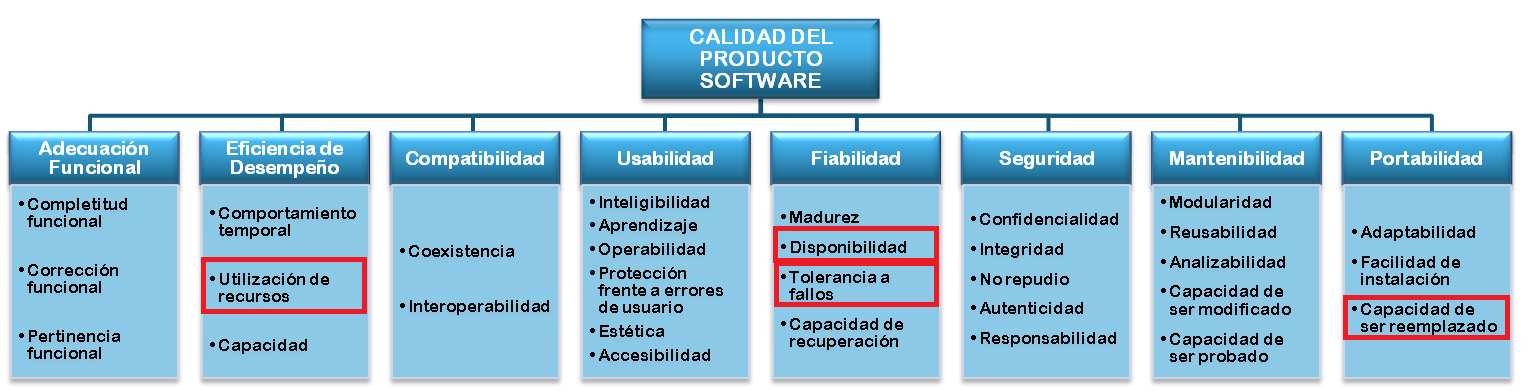
\includegraphics[scale=0.5]{iso25010}
\caption{Características y subcaracterísticas definidas en el modelo de calidad del producto de la ISO/IEC 25010 \cite{Standard2010}.}
\label{fig:iso25010}
\end{figure}

La figura \ref{fig:iso25010} muestra la división en características y subcaracterísticas del modelo de calidad del producto definido por la ISO/IEC 25010, resaltando aquellos que a continuación estudiaremos por su relación con los microservicios. Requisitos no funcionales asociados a atributos de calidad como la disponibilidad, la tolerancia a fallos, la utilización de recursos o la capacidad de ser reemplazado pueden conducir al arquitecto hacia la elección de una arquitectura basada en microservicios:

\begin{itemize}

\item La \textbf{disponibilidad} se define en la ISO/IEC 25010 como la capacidad del sistema de estar operativo y accesible para su uso cuando se requiere \cite{Standard2010}. En los sistemas distribuidos existen 3 características sobre las que se debe hacer balance: la consistencia, que establece que vamos a obtener una respuesta correcta de cualquier nodo de un servicio de acuerdo a su especificación, la disponibilidad, que ya hemos definido, y la tolerancia a particiones, que es la habilidad de gestionar situaciones en las que la comunicación entre las partes de un sistema se interrumpe. El teorema de CAP (debe sus siglas a las características en inglés \textit{Consistency}, \textit{Availability} y \textit{Partition Tolerance}) establece que en caso de fallo, solo dos de las tres características pueden prevalecer \cite{Gilbert2012}. En la siguiente sección entraremos en más detalle sobre el balance que se debe realizar para elegir que propiedad se debe sacrificar.

\item La \textbf{tolerancia a fallos} se define como la capacidad del sistema para operar según lo previsto en presencia de fallos hardware o software \cite{Standard2010}. Cuando se escala un sistema, la probabilidad de fallo es inevitable. Muchas organizaciones invierten mucho esfuerzo en evitar que un fallo se produzca, pero muy poco en mecanismos para recuperar el sistema una vez se ha producido. Un sistema que por culpa de un servicio caído deja de funcionar es menos resiliente que un sistema que puede continuar ofreciendo el resto de sus funcionalidades.

\item La \textbf{utilización de recursos} se define en la ISO como la cantidad y tipos de recursos empleados durante el funcionamiento del software bajo unas condiciones determinadas \cite{Standard2010}. Por un lado, los arquitecturas basadas en microservicos ofrecen beneficios ya que permiten que cada servicio se despliegue en un hardware diferente con unas prestaciones acordes a sus necesidades. También permiten que se escale cada servicio de acuerdo a su demanda de forma independiente, en lugar de tener que escalar el sistema monolítico al completo \cite{DelaTorre2018}. Por otro lado, los servicios se ejecutan en diferentes procesos y las llamadas interprocedurales a través de la red suponen un mayor consumo de recursos \cite{FowlerSusan}.

\item La \textbf{capacidad para ser reemplazado} es la capacidad de un producto software para ser reemplazado por otro en el mismo entorno y con el mismo propósito. La ventaja de los microservicios es que, gracias a su diseño modular, las piezas de software se pueden reemplazar fácilmente. Cada microservicio es un componente de software que puede ser completamente reescrito en poco tiempo. Autores como Jon Eaves \cite{Eaves2014} estiman que el tiempo para hacerlo no debería superar las dos semanas. Esto hace que se pueda reaccionar a situaciones imprevistas más fácilmente. Por ejemplo, para que un sistema pueda operar en un entorno determinado puede ocurrir que se tenga que reescribir un servicio por otra persona a la que inicialmente lo desarrolló. Al reescribirlo se puede hacer uso de otro lenguaje de programación; basta con mantener la misma interfaz del servicio para que otros puedan continuar operando con él. Si en lugar de reescribir un servicio se tuviera que reescribir toda la aplicación, el proceso de hacerlo no se podría abordar de forma incremental si la aplicación fuera un monolito.

\end{itemize}

\subsection{El teorema de CAP}

Pongamos un ejemplo en el que un microservicio está replicado y se produce un fallo por el cual la comunicación entre las replicas se interrumpe y los cambios en una replica no se pueden propagar al resto. Los \textbf{sistemas AP} son los sistemas que surgen fruto de sacrificar la consistencia cuando un fallo se produce, mientras que en los \textbf{sistemas CP} se pierde la disponibilidad. 

En el primer tipo, las replicas continuarían operativas, pero como los datos entre las replicas no se sincronizan se pueden obtener datos incorrectos al hacer una consulta. Cuando la comunicación se restablece, los cambios entre las replicas se sincronizarán. En los sistemas CP, para mantener la consistencia entre las replicas se tiene que rechazar cualquier petición, con lo que el servicio deja de estar disponible.

Los sistemas AP escalan más fácilmente y son más sencillos de construir, pero nos obligan a una consistencia eventual de los datos. Los segundos son los únicos que nos aseguran una consistencia fuerte, pero son más difíciles de construir. A la hora de optar por una solución u otra se debe tener en cuenta la especificación de requisitos, donde se debe detallar de forma específica y cuantitativa cuánto tiempo puede nuestro servicio estar inoperativo o con un dato obsoleto. Si en las actividades posteriores se opta por una arquitectura basada en microservicios, no será necesario implementar el sistema completo de una u otra forma. Cada microservicio tendrá necesidades diferentes y podrá seguir la aproximación que mejor le convenga \cite{Newman2015a}.

\section{Los microservicios en el diseño del sistema} \label{sct:FaseDiseño}

En la actividad de diseño se definen la arquitectura, componentes e interfaces del sistema. La especificación de requisitos es analizada para producir una descripción de la estructura interna del sistema, con el suficiente nivel de detalle para que sirva como base en su construcción. Diferentes diseños se plantean como alternativas, entre las que se debe hacer balance. Los modelos que se generan se destinarán a validar que se cumplen los requisitos establecidos y para planificar la implementación del sistema \cite{Bourque2014}.

\subsection{Librerías versus servicios} \label{subsect:librerias}

Un componente es una unidad de software que se puede reemplazar y actualizar de forma independiente. Las \textbf{librerías} son componentes que están ligados a un programa y son invocadas a través de llamadas a funciones. En cambio, los \textbf{servicios} son componentes que se ejecutan como procesos externos y con los que se puede comunicar a través de mecanismos como llamadas a procedimientos remotos (RPC) o peticiones HTTP \cite{Lewis2014}.

Uno de los motivos por los que se recomienda emplear servicios frente a librerías es que los servicios se pueden desplegar de forma independiente. Solo algunos cambios en la interfaz o contrato del servicio requerirán un cambio en sus consumidores. Además, algunas librerías obligan al uso específico de una tecnología. Sin embargo, las llamadas remotas son más costosas que las invocaciones dentro del mismo proceso, por lo que la interfaz del servicio debe definirse de tal forma que sus consumidores no tengan que comunicarse con él continuamente.

\subsection{Diseño guiado por el dominio (DDD)}

El \textbf{diseño guiado por el dominio} (DDD) \cite{Vaughn2013} es un enfoque para el desarrollo de software que propone un modelado rico, expresivo y evolutivo basado en la realidad del negocio. El dominio representa lo que hace una organización y la forma en que lo hace.

Con esta aproximación los expertos del dominio y los desarrolladores se sitúan en el mismo nivel empleando un \textbf{lenguaje ubicuo}. No hace falta ninguna traducción de términos entre ellos porque todos hablan un lenguaje común, que se plasma hasta en el código de programación. El lenguaje no tiene porque seguir los estándares de la industria que representa: utiliza los términos y acciones que en el negocio se dan.

El lenguaje ubicuo que se usa crece y cambia con el paso del tiempo. Nadie es capaz de conocer el dominio de un negocio completo porque este forma parte de un proceso de descubrimiento continuo. Si la organización sigue una estrategia de desarrollo ágil, en cada iteración se refina el modelo de forma incremental y este plasma en todo momento el software en funcionamiento.

Para su tratamiento, las áreas independientes del dominio se transforman en \textbf{contextos delimitados}. Cada contexto delimitado es un límite explícito que tiene su propio lenguaje ubicuo. Un concepto tiene un significado dentro de un contexto delimitado, pero fuera de él puede tener un significado totalmente distinto. Además, dentro del mismo dominio se puede usar el mismo nombre para un concepto en distintos contextos, pero con significados diferentes en cada uno. No se puede tratar de incluir todos los conceptos en un único contexto: se deben separar los conceptos en diferentes contextos y entender las diferencias que existen para un concepto llamado igual en uno y otro contexto.

\begin{figure}[h]
\centering
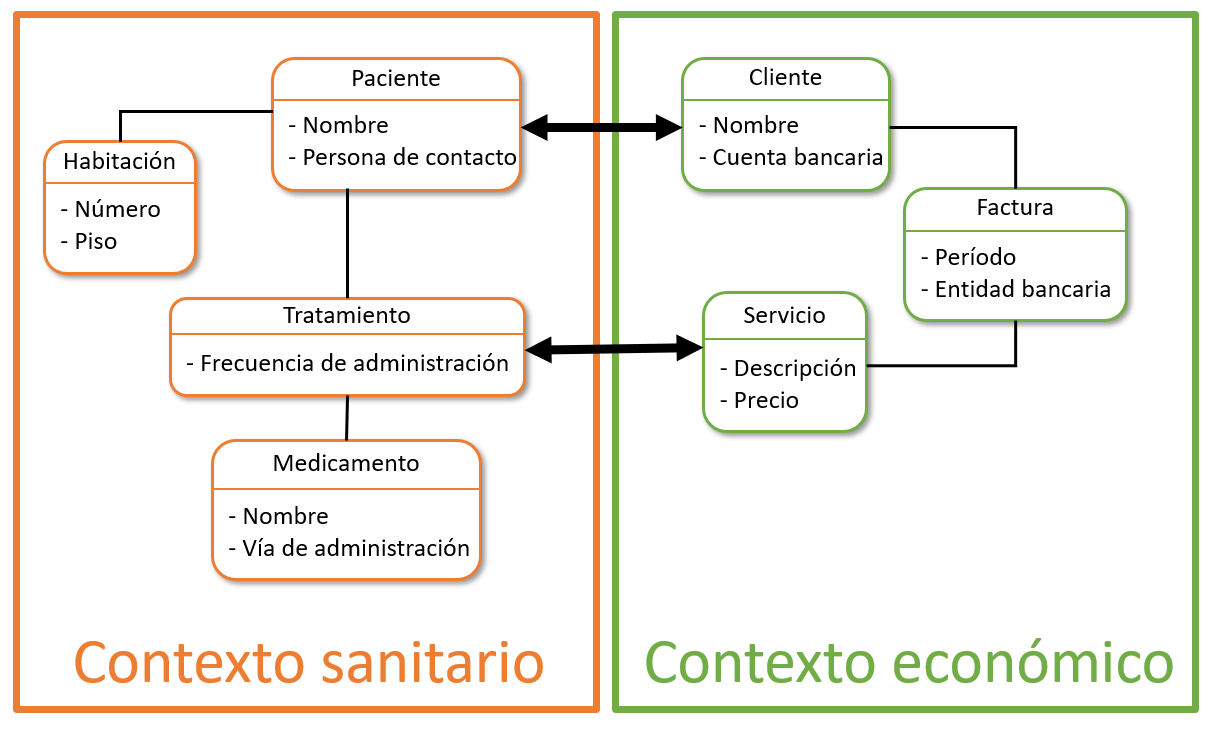
\includegraphics[scale=0.6]{BoundedContexts}
\caption{Ejemplo de dos contextos delimitados.}
\label{fig:BoundedContexts}
\end{figure}

En la figura \ref{fig:BoundedContexts} se han modelado dos contextos delimitados. En el ejemplo se observan los conceptos paciente y cliente, que representan a una única persona del mundo real, pero que se representa como una entidad distintas en cada contexto. Cada contexto nombra al mismo concepto de forma diferente, pero ambos están relacionadas. En cada uno, las entidades cuenta con unos atributos únicos asociados al contexto, como son la cuenta bancaria en el contexto económico o la persona de contacto en el sanitario. Estos atributos están ocultos fuera del contexto donde se localizan. Otros atributos como el nombre está presente en ambos contextos, lo que puede traer problemas de consistencia. 

Un cambio en el nombre de un paciente debe propagarse al nombre del cliente en el otro contexto. En los microservicios, cada servicio cuenta con su propia base de datos y propagar este tipo de cambios puede suponer un problema si uno de los que debe actualizarse está inoperativo. Para solventar este problema, se puede hacer que los atributos comunes solo se puedan modificar desde uno de los servicios donde está modelado y que los cambios al otro servicio se transfieran a través de una cola. 

Cada contexto está formado por modelos que no necesitan ser compartidos con otros a menos que se defina explícitamente una interfaz para que los empleen. La interfaz es el punto de entrada para que otros contextos puedan comunicar con el nuestro, empleando los términos y entidades que en nuestros modelos se definan.

Esta perspectiva puede trasladarse fácilmente al modelado de microservicios. Los contextos delimitados que analicemos en nuestro sistema son firmes candidatos a transformarse en servicios. Así, los límites de un servicio quedan bien limitados porque  todas las entidades que pueda requerir se encuentran dentro de sus fronteras, garantizándose su alta cohesión y bajo acoplamiento \cite{Newman2015a}.

\subsection{Descomposición en microservicios} \label{subsect:Descomposicion}

Cuando se razona sobre los límites de un servicio no se debe pensar en los datos que este almacena sino en las funcionalidades que ofrece. Pensar en los datos que almacena nos conduce a desarrollar únicamente servicios CRUD (en inglés, aquellos que nos permiten las operaciones de crear, leer, actualizar y eliminar datos), que ofrecen unas operaciones muy limitadas. Un servicio ofrece ciertas funcionalidades o capacidades que aportan \textbf{valor al negocio}.

Una descomposición temprana de un sistema en microservicios puede conllevar ciertos riesgos. Si el equipo a cargo del desarrollo tiene pocos conocimientos del dominio del problema a resolver, puede  ser buena idea comenzar la implementación como si de un sistema monolítico se tratara. Un mal diseño inicial puede desenvocar en que dos servicios se tengan que combinar porque exista un exceso de interacciones entre ellos. 

Es aconsejable dividir la solución en grandes servicios que poco a poco se vayan dividiendo en más pequeños conforme se estudien las ventajas de hacer cada nueva extracción. Una vez sean conocidos los límites de cada servicio, se pueden refactorizar los datos y el código hacia una granularidad más fina. Como se puede ver en la figura \ref{fig:refactoring}, se puede migrar primero solo la funcionalidad del servicio sin preocuparse por sus límites en base de datos para no tener que realizar simultáneamente dos migraciones. Una vez nos aseguremos de que el microservicio funciona correctamente, podemos migrar sus datos a una base de datos diferentes ya que cada microservicio ha de ser dueño de sus propios datos \cite{Richards2016}.

\begin{figure}[h]
\centering
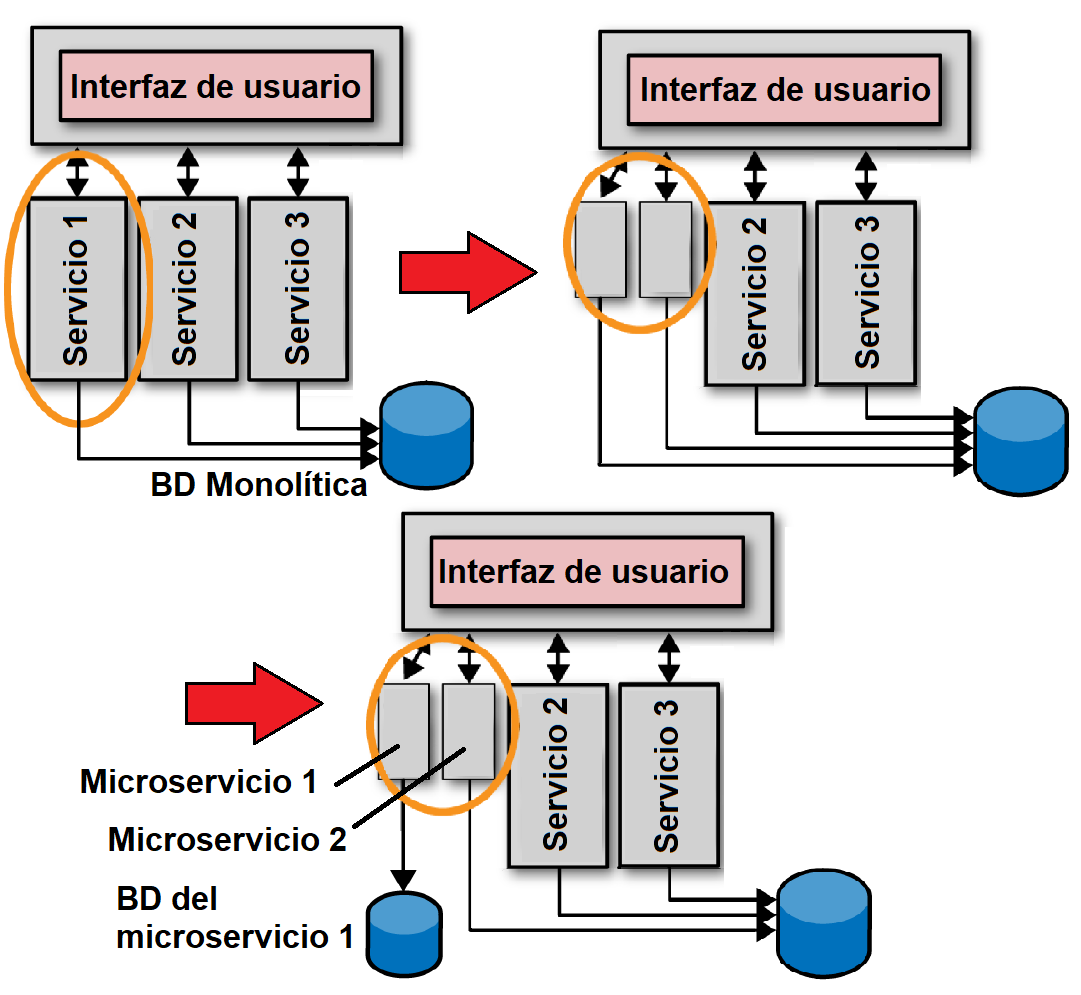
\includegraphics[scale=0.45]{refactoring}
\caption{Descomposición de un servicio en dos \cite{Richards2016}.}
\label{fig:refactoring}
\end{figure}

Cuando sea necesario realizar un cambio por nuevos requisitos del negocio, estos se localizarán en un contexto bien delimitado porque existirá una correspondencia entre la estructura de la organización y los microservicios del sistema. Como consecuencia, el tiempo medio para realizar un cambio se verá reducido porque solo hará falta volver a desplegar una porción del sistema. Además, la comunicación entre microservicios se asemejará a la existente entre las entidades del negocio.

\subsection{La tarea del arquitecto de software}

El software ha de ser diseñado para ser flexible, adaptarse y evolucionar en función de los requisitos de los usuarios. En lugar de centrarse en diseñar un producto final perfecto, el arquitecto debe crear un entorno donde el sistema correcto pueda emerger creciendo progresivamente a medida que se descubren nuevos requisitos. Gracias a su modularidad, los microservicios son el entorno perfecto para que esto ocurra.

El arquitecto de software debe preocuparse más por cómo interaccionan los servicios entre ellos y no tanto en lo que ocurre dentro de sus límites. En organizaciones grandes, cada microservicio puede estar desarrollado por un equipo distinto y es el arquitecto quien debe hacer de puente entre ellos \cite{Newman2015a}.

Una de las ventajas de las arquitecturas basadas en microservicios es la \textbf{heterogeneidad tecnol\'ogica}: cada servicio puede ser desarrollado empleando una pila tecnológica distinta. No obstante, dejar plena libertad a cada equipo para elegir la tecnología del servicio que va a desarrollar puede traer problemas a la hora de integrarlo con el resto del sistema. El uso de contratos o establecer normas en aspectos clave como el protocolo de comunicación entre los servicios facilitará su consumo. Las decisiones de diseño de un servicio en particular pueden recaer en el equipo responsable. En este caso, el arquitecto solo juega un papel de supervisor y asesor para evitar que se pierda la imagen del sistema completo.

\section{Los microservicios en la implementaci\'on del sistema}

La actividad de implementación consiste en la creación de un sistema o componente software combinando técnicas de programación, verificación y depuración. Esta actividad hace uso de los modelos producidos durante el diseño del sistema y sirve como entrada para la de pruebas. Los límites entre estas tres actividades varían en función del proceso seguido \cite{Bourque2014}.

\subsection{Integración de microservicios} \label{subsect:Integracion}

La \textbf{integración} es la parte más relevante en los sistemas basados en microservicios. Hacerlo correctamente nos asegurará su autonomía y su despliegue de manera independiente.

Por un lado, la tecnología empleada para la comunicación entre servicios no debe restringir la tecnología que en en estos se utiliza. Por otro lado, los consumidores deberían de tener total libertad para seleccionar la tecnología que utilizan y consumir un servicio para ellos no debe ser complejo de implementar. Además, los consumidores no deben conocer detalles internos del servicio que consumen para garantizar que estén desacoplados \cite{Newman2015a}. Existen muchas técnicas para la integración entre las que destacan: 

\begin{itemize}

\item \textbf{RPC} (\textit{Remote Procedure Call}): la llamada a procedimiento remoto es una técnica que permite ejecutar una llamada a un servicio como si de una llamada local se tratara. No es necesario que cliente y servidor empleen la misma pila tecnológica, aunque algunas tecnologías como Java RMI (\textit{Remote Method Invocation}) sí lo requieren. 

El formato de los mensajes también varía de una tecnología a otra. SOAP (proviene del inglés \textit{Simple Object Access Protocol}) emplea XML (también del inglés \textit{eXtensible Markup Language}) mientras que por ejemplo Java RMI transmite mensajes binarios.

\item \textbf{REST} (\textit{Representational State Transfer}): la transferencia de estado representacional es un estilo arquitectónico inspirado en la Web. Se basa en el concepto de recurso, un objeto que el servicio conoce y del que puede crear diferentes representaciones bajo demanda. La representación del recurso está completamente desacoplada de como se almacena.

La arquitectura REST es ampliamente usada junto con HTTP (término que proviene del inglés \textit{Hypertext Transfer Protocol}). Los verbos que se definen en HTTP actúan sobre recursos: por ejemplo, con el verbo GET se puede obtener una representación del recurso y con el POST crear uno nuevo.

\item \textbf{Integración basada en eventos}: en la integración basada en eventos, un servicio publica un evento cuando sucede algo relevante. Al evento se suscriben aquellos componentes que deben reaccionar al evento producido. Para hacer llegar los eventos a sus consumidores se debe mantener una nueva infraestructura, como puede ser una cola basada en mensajes.

\begin{figure}[h]
\centering
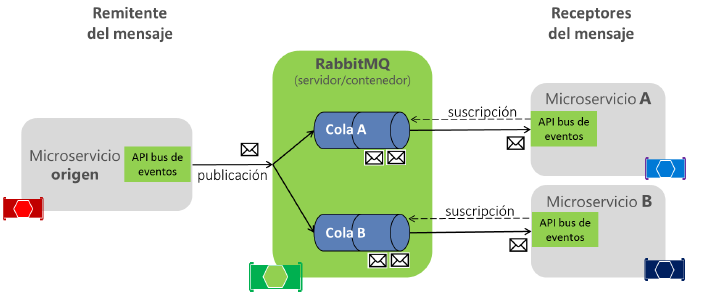
\includegraphics[scale=0.85]{rabbitmq}
\caption{Ejemplo de integración basada en eventos con un contenedor de RabbitMQ \cite{DelaTorre2018}.}
\label{fig:rabbitmq}
\end{figure}

Un bróker de mensajería es un patrón arquitectónico para la validación, la transformación y el enrutamiento de mensajes. RabbitMQ es un ejemplo de este patrón. En esta herramienta, el productor de un evento publica este a través de una API, donde será tramitado por el bróker para hacerlo llegar a todos los consumidores suscritos, como se representa en la figura \ref{fig:rabbitmq}. En el mismo servidor de RabbitMQ se pueden hospedar diferentes colas, haciendo que cada servicio solo se suscriba a la que le interesa (en el ejemplo, cada servicio se suscribe a una cola diferente).
 
\end{itemize}

Tanto SOAP como REST emplean HTTP, aunque solo el segundo hace uso de los verbos definidos en HTTP. Existen pocas librerías para trabajar con SOAP, mientras que prácticamente cualquier lenguaje de programación contemporáneo cuenta con un cliente HTTP, con soporte para más o menos verbos. En cuanto a su rendimiento, REST es más eficiente en términos de latencia y ancho de banda consumido \cite{Mulligan}. REST es más recomendable que SOAP para enviar grandes volúmenes de datos por ser más compacto y permitir formatos como el JSON o el binario. Sin embargo, ni uno ni otro son recomendables para trabajar en redes con latencias bajas porque usan HTTP. En este caso, es mejor emplear directamente protocolos como TCP o UDP. 

En cuanto al tercer tipo de integración, la integración basada en eventos fomenta la escalabilidad y resiliencia de los servicios y reduce el acoplamiento entre ellos. No obstante, requiere aprovisionar nuevas infraestructuras y añade complejidad a la hora de razonar sobre el sistema por ser una comunicación asíncrona. Algunas buenas prácticas para afrontar su complejidad van desde el uso efectivo de sistemas de monitorización hasta el uso de identificadores de correlación para trazar las llamadas entre servicios \cite{Newman2015a}. 

\subsection{Programación y persistencia políglotas} \label{subsec:Poliglota}

%TODO Sustituir anteriormente por enlace.
Como hemos comentado anteriormente, diferentes microservicios se pueden desarrollar empleando diferentes tecnologías. La base de datos que contiene los datos del servicio o la arquitectura interna del microservicio también pueden adaptarse a los requisitos del mismo \cite{DelaTorre2018}. La \textbf{programación políglota} se fundamenta en que diferentes lenguajes de programación son más aptos para tratar problemas específicos. Es más productivo escoger el lenguaje adecuado para un servicio concreto que tratar de buscar un lenguaje que se ajuste a los requisitos de todos.

\begin{figure}[h]
\centering
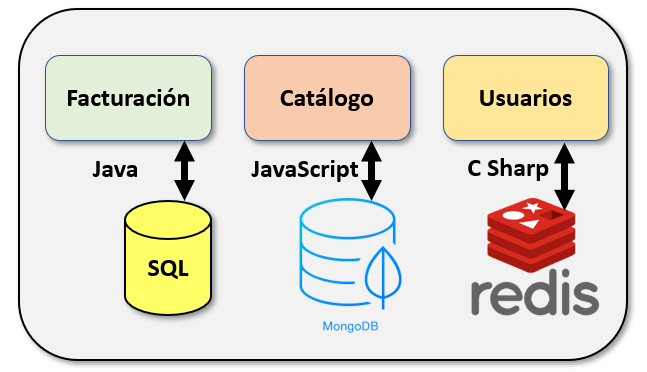
\includegraphics[scale=0.65]{poliglota}
\caption{Ejemplo de sistema políglota.}
\label{fig:poliglota}
\end{figure}

El término también se puede extrapolar a la persistencia. La \textbf{persistencia políglota} hace uso de diferentes tecnologías para la persistencia en función de los datos a almacenar y de cómo estos se van a manipular. Cada microservicio es dueño de sus datos y puede utilizar una tecnología diferente. Las bases de datos relacionales no son la única opción y se deben considerar otras que escalen mejor si el servicio recibe muchas peticiones o se quiere hacer una explotación eficiente de los datos \cite{Fowler2011}.

En ambos casos, se debe hacer balance entre los beneficios que puede aportar un diseño políglota y sus costes asociados, por ejemplo, de aprendizaje. En la figura \ref{fig:poliglota} se representa un sistema políglota donde se emplean diferentes lenguajes (Java, Javascript, C\#) y diferentes tecnologías de BD en diferentes microservicios.

\subsection{La ley de Conway \cite{Conway1968}}

Problemas asociados a bases de código inmensas donde colabora un gran equipo pueden ser evitados empleando microservicios. Si el código está repartido entre diferentes componentes, equipos pequeños pueden encargarse de mantener cada uno de ellos. De esta manera, la organización del trabajo adquiere un enfoque más ágil al estar formado por equipos independientes y auto-organizados \cite{Newman2015a}.

En las aplicaciones monolíticas, normalmente los equipos de trabajo que se forman están asociados la interfaz de usuario, la base de datos y la parte servidora. Cualquier cambio simple involucra la coordinación entre diferentes equipos. De acuerdo a la \textbf{ley de Conway}, una organización que diseña un sistema producirá un diseño para la aplicación que será una copia de su estructura organizacional \cite{Conway1968}. Así, es natural que la organización de los microservicios se realice de acuerdo con el negocio. Los equipos que se encargan de cada servicio son multifuncionales y se pueden autogestionar. En cada equipo están presentes, entre la totalidad de sus miembros, todas las habilidades necesarias para el desarrollo completo del servicio \cite{Lewis2014}.

\section{Los microservicios en la actividad de pruebas} \label{sect:FasePruebas}
% Art of unit testing
% Building microservices
% Simian army

Las pruebas de software consisten en la verificación de que un programa produce las salidas esperadas para un conjunto finito de casos de prueba. Los casos de prueba son finitos porque el número posible de pruebas es infinito y estos se seleccionan en función de la prioridad y riesgo del código bajo pruebas. Además, se debe comprobar la salida obtenida con el resultado esperado para comprobar si esta es o no aceptable \cite{Bourque2014}.

En esta sección presentaremos la clasificación de pruebas que Newman \cite{Newman2015a} realiza. Se enfoca en clasificar las pruebas en base a su alcance respecto a los microservicios que involucran, a diferencia de como se clasifican las pruebas tradicionalmente según las clases o métodos que se invocan.

\subsection{Pruebas unitarias}

Una \textbf{prueba unitaria} es una pieza de código que invoca al método o clase bajo prueba y que comprueba ciertas asunciones sobre su lógica. Se ejecutan de forma rápida y sencilla, están automatizados y son fácilmente mantenibles \cite{Osherove2014}. En general, se prefiere tener un gran número de este tipo de pruebas por su rapidez, porque pueden ayudar a la refactorización del código y porque es donde mayor cantidad de defectos se suele detectar.

\begin{figure}[h]
\centering
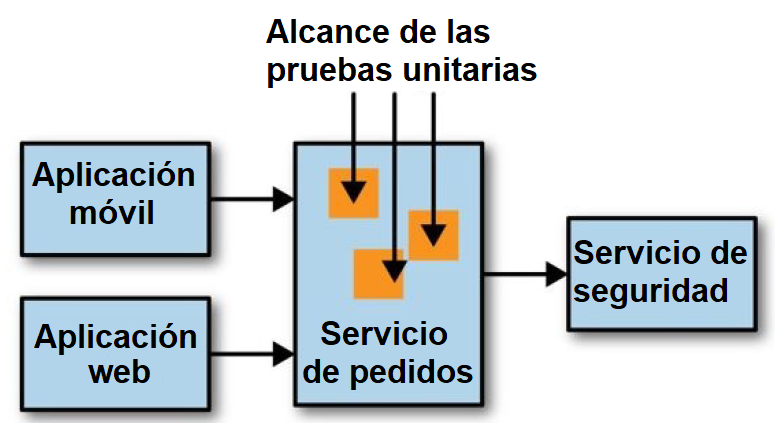
\includegraphics[scale=0.5]{Unit_Tests_ES}
\caption{Diagrama de pruebas unitarias.}
\end{figure}

\subsection{Pruebas de servicios}

En las \textbf{pruebas de servicios} se verifica cada una de las funcionalidades que un servicio expone. Se pretende verificar el servicio de forma aislada y para ignorar las dependencias que el servicio bajo pruebas tiene sobre otros se reemplazan los servicios colaboradores por \textit{fakes}. Un fake es un sustituto  de una dependencia que devuelve una respuesta predeterminada cuando el servicio bajo pruebas le solicita algo.

Encajan dentro de las pruebas de integración, que se definen como la prueba como un conjunto de dos o más módulos de software que colaboran para evaluar un resultado esperado \cite{Osherove2014}. Este tipo de pruebas pueden ser igual de rápidas que las unitarias siempre que no se tengan que emplear un gran número de infraestructuras como bases de datos o colas.

\begin{figure}[h]
\centering
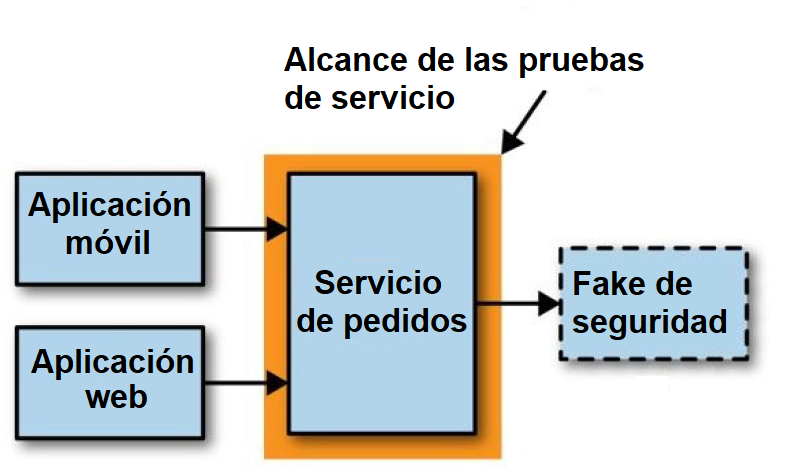
\includegraphics[scale=0.5]{Service_Tests_ES}
\caption{Diagrama de pruebas de servicios.}
\end{figure}

\subsection{Pruebas de extremo a extremo}

Las \textbf{pruebas de extremo a extremo} (en inglés, \textit{end to end} o E2E) \cite{Newman2015a} son pruebas que se ejecutan sobre todo el sistema. Cubren gran parte de código, por lo que su correcta ejecución dan mucho grado de confianza. En su ejecución se levantan varios servicios diferentes.

Son pruebas frágiles: conforme el alcance de la prueba aumenta más son las partes sobre las que no se puede tener control. Estas partes pueden introducir fallos que no demuestran que la funcionalidad tenga un defecto y hacen la prueba menos determinista. Si la prueba falla continuamente, el equipo encargado puede llegar a asumir como normal está situación. Su tiempo de ejecución es mayor y en consecuencia, más tarde se detecta si un cambio ha introducido un defecto \cite{Newman2015a}.

\begin{figure}[h]
\centering
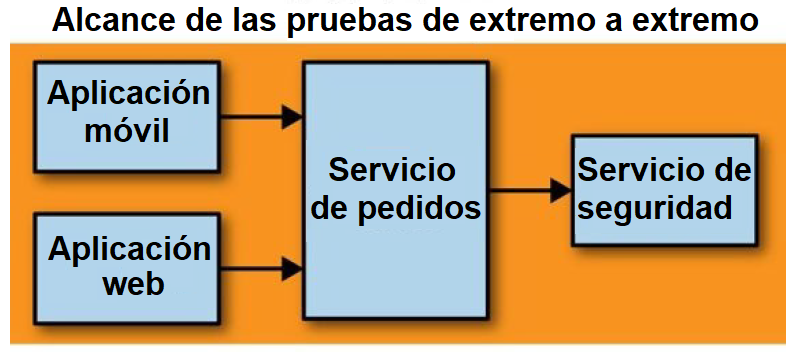
\includegraphics[scale=0.5]{End_To_End_Test_ES}
\caption{Diagrama de pruebas de extremo a extremo.}
\end{figure}

\subsection{Balance de pruebas a realizar}

A medida que aumenta el alcance de las pruebas lo hace el nivel de confianza que las pruebas dan sobre la ausencia de defectos. Por otro lado, cuanto más arriba en la pirámide de la figura \ref{fig:Cohn_Pyramid_ES} más tiempo tardará una prueba en implementarse y ejecutarse. Además, determinar el motivo de fallo de una prueba será más costoso cuanto mayor sean las líneas de código probadas \cite{Cohn2010}.

\begin{figure}[h]
\centering
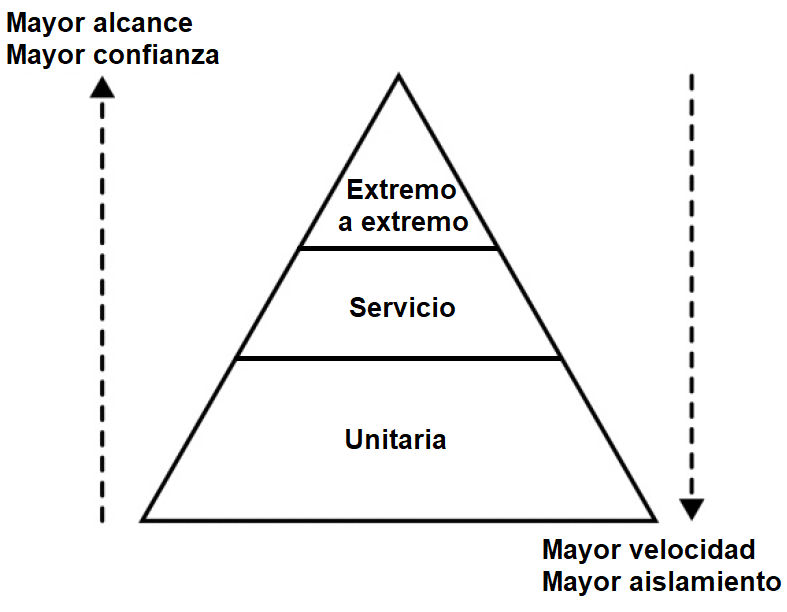
\includegraphics[scale=0.5]{Cohn_Pyramid_ES}
\caption{Pirámide de pruebas diseñada por Mike Cohn \cite{Cohn2010}.}
\label{fig:Cohn_Pyramid_ES}
\end{figure}

El número de pruebas que se aconseja tener de cada tipo aumenta conforme descendemos por la pirámide. El número de servicios que participan para ofrecer una funcionalidad al usuario puede ser muy alto y en una prueba no se deberían de levantar más de 3 o 4 servicios para no potenciar las desventajas que hemos mencionado. Por este motivo, las pruebas de extremo a extremo deben ser las mínimas posibles y se deben organizar en pruebas de servicios que empleen fakes siempre que se pueda.

\section{Los microservicios en el despliegue}
% Docker
% Kubernetes
% Orquestadores (¿Moltó?)
% Azure y AWS
% CI/CD

El despliegue se define como la entrega de software (como un producto completo o como resultado de un incremento en un desarrollo incremental) al cliente para que este lo evalúe y devuelva retroalimentación al equipo de desarrollo \cite{Pressman}. Debido a la naturaleza incremental de la mayoría de procesos de desarrollo, esta es una actividad que se realiza numerosas ocasiones. 

En cada despliegue, se debe proveer del soporte necesario para el empleo de las nuevas características. Además, la retroalimentación recibida guiará el proceso de desarrollo hacia las siguientes modificaciones y funcionalidades que se deben realizar.

Los problemas que aparecen en una nueva versión del producto deben ser atendidos. Para garantizar que estos no ocurran, se deben hacer pruebas en cuantos más entornos posibles mejor.

\subsection{Integración y entrega continua}

La \textbf{integración continua} es una práctica en el desarrollo de software donde los miembros del equipo integran su trabajo de forma frecuente, normalmente a diario. Cada integración se verifica mediante compilaciones automatizadas que incluyen la ejecución de pruebas para detectar errores y conflictos en la integración \cite{Fowler2006}. El término tiene su origen como una de las doce prácticas de la metodología \textit{Extreme Programming} (XP).

Durante este proceso se crean artefactos sobre los que se ejecutarán validaciones. Los artefactos construidos deben ser lo más parecidos a los que más tarde se despliegan en la versión de producción para asegurar que es el mismo artefacto sobre el que se han hecho las pruebas. Entre los beneficios de la integración continua encontramos:
 
\begin{itemize}

\item \textbf{Rápida retroalimentación}: los desarrolladores obtienen más rápido una respuesta sobre la calidad de sus cambios. Con este fin, la compilación ha de ser lo más rápido posible. Se pueden obtener mayores beneficios de la integración continua a través de las compilaciones por fases o \textit{build pipelines}. En este tipo de compilaciones se separa por pasos el proceso. Los pasos de la \textit{pipeline} pueden ser manuales, como las pruebas de aceptación de un usuario, o estar automatizados, como la ejecución de pruebas unitarias. La ventaja de hacer esto es que se obtiene una retroalimentación más rápida si se ejecutan de forma separada acciones rápidas de otras más pesadas \cite{Fowler2006}.

\item \textbf{Equipo sincronizado}: los integrantes de un equipo obtienen más rápido los cambios que otros han realizado y conocen en todo momento el estado de la compilación. Si esta falla, arreglarla es la prioridad número uno.

\item \textbf{Trazabilidad}: si el código está bajo control de versiones, en cualquier momento se puede volver a construir un artefacto de una versión concreta a partir del código que la origina \cite{Newman2015a}.

\end{itemize}

\begin{figure}[h]
\centering
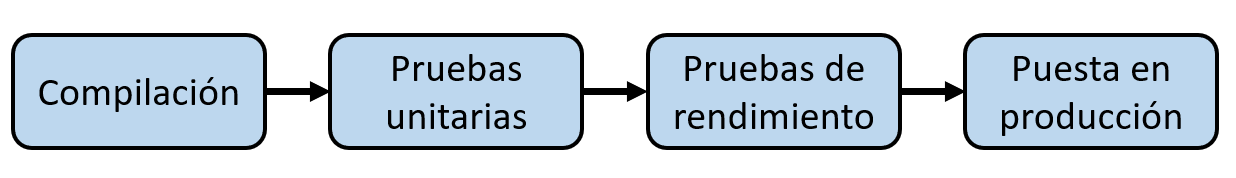
\includegraphics[scale=0.6]{pipeline_ES}
\caption{Ejemplo de una pipeline \cite{Newman2015a}.}
\end{figure}

La \textbf{entrega continua} extiende la idea de la integración continua en cuanto a que cada cambio que ha superado la compilación puede ser candidata para ser desplegada en producción en cualquier momento. Sobre cada cambio se puede decidir si se publica o no a producción y hacerlo no cuesta más que pulsar un botón porque está todo el proceso de despliegue automatizado. La práctica de que cada cambio que se realiza y supera la \textit{pipeline} es publicado automáticamente a producción se denomina \textbf{despliegue continuo} \cite{Fowler2013}.

\subsection{Virtualización y tecnología de contenedores}

Un \textbf{\textit{host}} representa una unidad genérica de aislamiento, un sistema operativo donde se pueden instalar y ejecutar servicios. Si desplegamos directamente sobre máquinas físicas, entonces un \textit{host} será el equivalente a una de ellas. Sin embargo, tener muchos \textit{hosts} es costoso si cada uno consiste en una máquina diferente \cite{Newman2015a}.

La \textbf{virtualización} nos permite dividir una máquina en \textit{hosts} separados, donde pueden ejecutarse servicios distintos. En la virtualización tradicional, cada una de las máquinas virtuales (MV) puede ejecutar su propio sistema operativo. Un recurso adicional es añadido entre la máquina física y las virtuales: el hipervisor. El hipervisor reparte recursos de la máquina física como la CPU o la RAM entre los distintos \textit{hosts} virtualizados y permite al usuario la gestión de las máquinas virtuales contenidas. En la figura \ref{fig:containers_vms_ES} se ilustra el hipervisor como una capa más entre los componentes desplegados y la máquina física.

El mayor inconveniente de las máquinas virtuales es que se puede dividir una máquina en muchas piezas como queramos porque la separación entre los hosts supone un coste. El hipervisor también consume recursos y cuantas más son las máquinas que debe gestionar, mayor será su consumo. Además, el tiempo de puesta en funcionamiento de una máquina virtual es de la magnitud de minutos, mientras que el arranque de un contenedor ronda los pocos segundos. \cite{Dua2014} Esto es muy importante en desarrollos que siguen las técnicas de integración continua donde se despliegan artefactos frecuentamente. 

Los \textbf{contenedores} son sistemas operativos ligeros que se ejecutan sobre una máquina con la que comparten el \textit{kernel}. El número de contenedores que una máquina puede alojar es mayor que el número de máquinas virtuales debido a la naturaleza ligera de estos \cite{Dua2014}. Su uso de recursos y tiempo de aprovisionamiento son menores al de una MV, lo que reduce el tiempo de retroalimentación sobre el funcionamiento de un servicio. Sin embargo, el grado de aislamiento de los contenedores no es perfecto ya que existen formas en las que se puede interferir en el funcionamiento de otro contenedor debido a problemas de diseño y bugs conocidos \cite{Newman2015a}.

\begin{figure}[h]
\centering
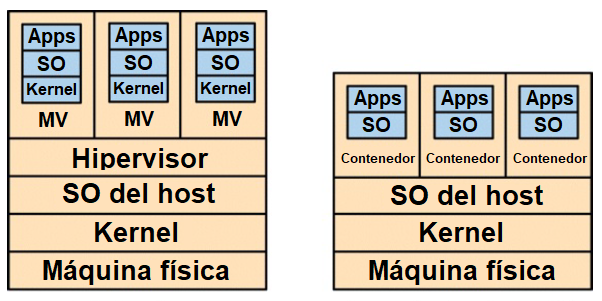
\includegraphics[scale=0.8]{containers_vms_ES}
\caption{Comparación entre la virtualización y la contenerización \cite{Newman2015a}.}
\label{fig:containers_vms_ES}
\end{figure}

Ambas soluciones se pueden combinar para obtener las ventajas de las dos. Se puede obtener una máquina virtual de una plataforma como Amazon Web Services (AWS) que nos asegure características como la escalabilidad bajo demanda y sobre ella ejecutar diferentes servicios desplegados como contenedores.

\section{Los microservicios en la fase de mantenimiento}
% You code, you run it -> Buscar documento "oficial"
% Monitorización
% Arquitectura evolutiva

Los productos software cambian y evolucionan. Una vez están desplegados en el entorno donde operan se dan situaciones en las que se detectan errores o los requisitos de los usuarios se ven modificados. Es una fase que debe comenzar de forma temprana para garantizar la mantenibilidad del sistema a desarrollar \cite{Bourque2014}.

El mantenimiento de software es la fase del desarrollo que más recursos consume, alrededor del 60\% o 70\% del coste original de un proyecto. La mayoría del software que hoy se emplea tiene entre 10 y 15 años, tiempo en el cual ha sufrido muchas modificaciones hasta alcanzar un diseño pobre y difícil de mantener. Se puede definir el software mantenible como aquel que se diseña de forma modular, siguiendo patrones de diseño y estándares de calidad y que se documenta de tal forma que es explicativo por si mismo \cite{Pressman}.

Gracias a su diseño modular, los microservicios son una arquitectura que se puede seguir para hacer más sencillo el mantenimiento de un sistema. Sin embargo, las consecuencias de elegir un estilo arquitectónico no son evidente hasta años más tarde de haber sido desarrollado, por lo que hasta que no se vean sistemas maduros que empleen microservicios no se debe afirmar a ciencia cierta que garantizan estas características. \cite{Lewis2014}

\subsection{Refactorización}

%TODO Característica del ISO 25010

En la mayoría de empresas abundan los sistemas legados que nadie desea mantener. La \textbf{refactorización} de estos sistemas suele ser muy difícil por su tamaño y riesgo. Si en lugar de haber seguido una arquitectura monolítica para su diseño se emplearan microservicios se observaría como los barreras para la refactorización no existen al poderse reescribir el microservicio al completo en pocos días. \cite{Eaves2014}

\subsection{\textit{You Build It, You Run It}}

En muchas organizaciones, el desarrollo de sistemas se hace a través de proyectos: piezas de software que una vez desarrolladas se consideran completadas. En una aproximación basada en microservicios, cada equipo es responsable del ciclo de vida completo de un producto o servicio. Esto sigue la filosofía de Amazon: \textbf{\textit{``you build it, you run it"}} \cite{Lewis2014}.

No hay necesidad de distinguir entre quien construye un sistema y quien lo ejecuta y posteriormente mantiene. Esta filosofía aproxima a desarralloradores y clientes: los desarrolladores están en contacto directo con los clientes día tras día, lo que les proporciona retroalimentación para mejorar la calidad de sus servicios. Tampoco hay necesidad de contar en la organización con un equipo centrado en la infraestructura (IT). Contar con un equipo así distribuye la responsabilidad de hacer un servicio funcionar entre diferentes equipos y añade un sobresfuerzo de coordinación y comunicación cuando un problema aparece \cite{Vliet2011}.

\subsection{Documentación y deuda técnica}

Una de las ventajas de los microservicios es que acelara el proceso de desarrollo. Sin embargo, cuanto más rápido tratamos de implementar un servicio más probable es que tomemos atajos para poder desplegar antes una iteración del producto, lo que se traduce en un aumento de la \textbf{deuda técnica} \cite{FowlerSusan}. La deuda técnica \cite{Garzas} se puede definir como el sobresfuerzo que debe llevarse a cabo por  haber tomado una mala decisión en el desarrollo del software.

En un equipo de desarrollo el conocimiento de cómo funciona un sistema se reparte entre los miembros que lo forman. Nadie es capaz de conocer completamente su funcionamiento y lo más probable es que cada desarrollador conozca mejor la parte donde más tiempo ha invertido. A la hora de realizar un cambio, el entendimiento de cómo funciona el sistema tiene que ser compartido por todos sus miembros para asegurar que el cambio a implementar es el correcto.

La documentación es una de las mejores maneras de solventar la deuda técnica y garantizar que el equipo de desarrollo conoce realmente cómo funciona un microservicio. Cabe recordar que cada microservicio puede seguir una arquitectura diferente o utilizar una tecnología distinta. Debido a esto, se debe documentar de forma exhaustiva para facilitar la integración entre ellos y facilitar el traslado de personas de un equipo a otro.

\subsection{Monitorización}

Durante el mantenimiento se debe asegurar la disponibilidad de los microservicios. Las herramientas de monitorización son clave para garantizar los \textbf{acuerdos de nivel de un servicio} (SLA) y el estudio de errores cuando estos ocurren.

Con este fin, se debe registrar toda aquella información relevante que ocurra. Los microservicios colaboran entre ellos para ofrecer funcionalidades concretas y recrear un sistema donde ha ocurrido un error puede ser complejo debido a que cada uno se versiona de forma independiente. Por ello, lo mejor es contar con toda la información necesaria registrada para determinar la causa del problema.

La información más útil se debe mostrar de forma gráfica a través de \textit{dashboards} que reflejen el estado de salud de los servicios. Así, la informacón más consultada se puede visualizar de forma rápida y fácil de entender para ahorrar tiempo. No obstante, cuando un problema ocurre se debe hacer uso de alertas para atenderlo de forma prioritaria. Estas alertas han de ser accionadas automáticamente por métricas que superen un límite establecido, como puede ser el uso de recursos, o por la ocurrencia de excepeciones en el servicio \cite{FowlerSusan}. 

%%%%%%%%%%%%%%%%%%%%%%%%%%%%%%%%%%%%%%%%%%%%%%%%%%%%%%%%%%%%%%%%%%%%%%%%%%%%%%%
%              					Estado del arte
%
%%%%%%%%%%%%%%%%%%%%%%%%%%%%%%%%%%%%%%%%%%%%%%%%%%%%%%%%%%%%%%%%%%%%%%%%%%%%%%%

\chapter{Estado del arte de la tecnología de microservicios}

\section{Contenedores}

Un contenedor \cite{Hunter2017} es una unidad de aislamiento que existe dentro de un sistema operativo. Mientras que una máquina virtual requiere tener su propio SO, un contenedor puede acceder al sistema operativo de la máquina donde reside, eliminando la necesidad de tener sistemas operativos redundantes. En esta sección revisaremos dos de los más empleados: los contenedores Docker y los contenedores Linux. Existen otros contenedores, como los contenedores Warden y OpenVZ. Si se desea obtener más información sobre ellos, en \cite{Dua2014} se realiza una comparación entre todos ellos en cuanto al aislamiento que ofrecen y su ciclo de vida.

\subsection{Contenedores Linux}

Los \textbf{contenedores Linux} (LXC) \cite{Amaral2016} permiten crear un espacio de procesos separado en el que puede ejecutarse de forma aislada un servicio. Cada contenedor es un subárbol del principal y puede tener asociado recursos físicos gestionados por el kernel \cite{Newman2015a}.

Estos contenedores se fundamentan en los espacios de nombre de Linux y los grupos de control (\textit{cgroups}). Los espacios de nombre disminuyen el conjunto del sistema de archivos que un grupo de procesos puede ver. Los grupos de control organizan los procesos en un árbol de forma jerárquica, donde se pueden definir límites y políticas para el uso de los recursos \cite{Amaral2016}.

La principal ventaja de los LXC es que son una implementación muy ligera que se ejecuta a velocidades muy similares a las de la máquina donde se despliegan. Sin embargo, limitan al uso de Linux como base del entorno porque están muy acoplado a su kernel. También presentan problemas en cuanto a la seguridad y aislamiento de los contenedores \cite{Dua2014}. 

Una solución a estos problemas pasa por usar contenedores Linux desplegados en máquinas virtuales. De esta forma, los límites de seguridad se establecen a nivel de la MV mientras que los límites de los recursos empleados por la aplicación se establecen en base a sus contenedores \cite{DeAlfonso2017}.

\subsection{Docker}

Docker \cite{Matthias} es una herramienta basada en contenedores Linux para la creación de artefactos que se pueden desplegar en cualquier entorno y se pueden distribuir y escalar bajo demanda. Su funcionamiento es sencillo: en un fichero llamado \textbf{Dockerfile} se especifican las dependencias del servicio en distintos pasos y un comando que inicia el servicio. De la compilación del Dockerfile se origina una \textbf{imagen}: un paquete con todas las dependencias e información necesaria para crear un contenedor. Las imágenes permiten empaquetar un servicio para desplegarlo de forma confiable y reproducible tantas veces como se desee \cite{DelaTorre2018}.

La filosofía de Docker se centra en los contenedores desechables. Nada en el entorno donde se ejecuta la aplicación permanecerá ahí más allá de lo que viva la aplicación. Esto implica que no se delegará en entornos donde se encuentra casualmente una dependencia no especificada en la imagen. Docker promueve las arquitecturas sin estado (\textit{stateless}) o que externalizan este a otras infraestructuras como bases de datos. Las aplicaciones así se hacen más portables, escalables y confiables \cite{Matthias}.

El proceso de desarrollo también se simplifica: en aproximaciones como la de microservicios, un equipo encargado de un servicio solo necesita la imagen de otro para integrarlo con el suyo y no necesita conocer detalles internos de este. Además, las tareas de construcción de la imagen, provisión de la configuración y despliegue pueden ser realizadas por diferentes personas, como se muestra en la figura. Este flujo de trabajo se representa en la figura \ref{fig:docker_process_ES}, donde dos equipos se dividen las tareas para publicar un contenedor en producción. 

\begin{figure}[h]
\centering
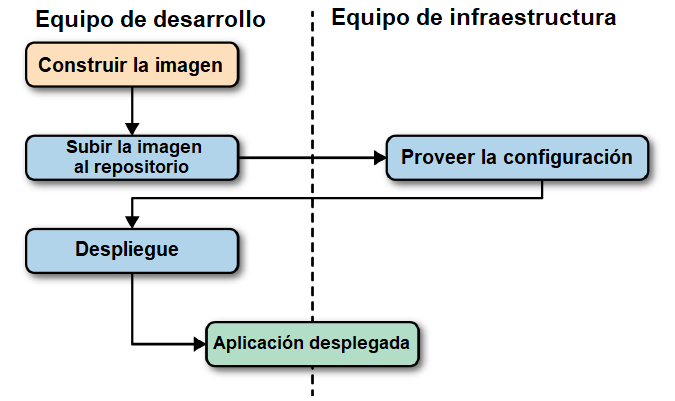
\includegraphics[scale=0.7]{docker_process_ES}
\caption{Proceso de despliegue con Docker \cite{Matthias}.}
\label{fig:docker_process_ES}
\end{figure}

Si se integra dentro del proceso de despliegue, cada cambio que pasa por una \textit{pipeline} puede construir una nueva imagen Docker. Sobre ella se ejecutarán pruebas de forma automatizada para después ser publicada a producción. De esta forma, el equipo puede asegurarse de que el artefacto sobre el que se han ejecutado las pruebas es el mismo que se publica más tarde. 

%%%%%%%%%%%%%%%%%%%%%%%%%%%
% SALTO DE PAGINA
%%%%%%%%%%%%%%%%%%%%%%%%%%%
\newpage

\section{Orquestadores}
%TODO https://medium.com/@PamRucinque/qu%C3%A9-es-eso-de-serverless-f4f6c8949b87
%TODO https://rancher.com/load-balancing-in-kubernetes/

Un orquestador \cite{DelaTorre2018} es una herramienta para la gestión de clústeres y contenedores. Permiten gestionar las imágenes que originan los contenedores, los \textit{hosts}, las redes de contenedores, el balanceo de carga o el descubrimiento de servicios. De nuevo, nos centraremos solo en dos: Kubernetes y Docker Swarm. Estos son los dos más empleados por la industria, aunque podemos nombrar otros como  Apache Mesos.

\subsection{Kubernetes} \label{subsect:Kubernetes}
%TODO Definir cluster.
%TODO Rancher. 
Kubernetes \cite{Rensin2015} es una herramienta diseñada por Google para el despliegue y orquestación de aplicaciones en contenedores Docker de forma resiliente. Cada una de las máquinas que aloja uno o más contenedores Docker se denomina \textbf{nodo}. La unidad más pequeña con la que trabaja Kubernetes no son los contenedores, sino los pods. Un \textbf{pod} es una colección de contendores y volúmenes agrupados juntos en un nodo. Los \textbf{volúmenes} son sistemas de archivos virtuales que se pueden emplear para comunicar entre ellos a los contenedores de un nodo. Kubernetes orquesta a nivel de los pods, por lo que dos contenedores en el mismo pod serán administrados igual. La relación de continencia entre estos componentes se plasma en la figura \ref{fig:kubernetes_ES}.

\begin{figure}[h]
\centering
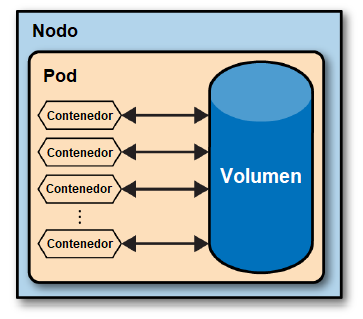
\includegraphics[scale=0.9]{kubernetes_ES}
\caption{Un nodo de Kubernetes \cite{Rensin2015}.}
\label{fig:kubernetes_ES}
\end{figure}

Kubernetes se emplea principalmente para especificar el número de replicas que se desea tener simultánemanete de un pod. La herramienta es buena para asegurar la disponiblidad de un servicio, pero no garantizan la escalabilidad de esta, que consistiría en modificar el número de replicas de un pod de forma dinámica en función de su demanda. Para este propósito se deben introducir balanceadores de carga como puntos de entrada al sistema. Estos balanceadores redirigirían cada petición al pod correspondiente y se encargarán de ajustar el número de replicas de un pod según una serie de reglas.

En el apéndice \ref{chap:Despliegue} \nameref{chap:Despliegue} se dan algunos detalles más acerca de Kubernetes ya que es el orquestador empleado por el caso de estudio en el entorno de producción. Entre la información que aquí se puede encontrar está el uso de los servicios \textit{LoadBalancer} e \textit{Ingress}.

\subsection{Docker Swarm}

Docker Swarm \cite{DeAlfonso2017} es la aproximación nativa propuesta por Docker para la creación de clústeres. Un clúster consiste en un conjunto de contenedores Docker que aparentan formar uno único de forma virtual.

En cuanto a la arquitectura de Docker Swarm, los nodos ejecutan un agente para atender a los cambios en su configuración y uno de ellos ejecuta un gestor llamado \textit{Swarm} para la coordinación de los nodos. Cuando un contenedor es creado, este se despliega en cualquiera de los nodos gestionados por el Swarm. El conjunto de contenedores son gestionados por el \textit{Swarm} como una única entidad.

Docker Swarm se puede ejecutar para ofrecer servicios con alta disponibilidad a través de herramientas como etcd, Consul o ZooKeeper para la gestión y recuperación de los fallos. Además, está complementamenta integrado dentro de la interfaz de línea de comandos de Docker.

\section{Proveedores de servicios en la nube}

Un \textbf{proveedor de servicios en la nube} \footnote{ What is a cloud service provider?: \url{https://azure.microsoft.com/en-gb/overview/what-is-a-cloud-provider/}} es una compañía de terceros que ofrece servicios en la nube de plataforma (PaaS), infraestructura (IaaS), aplicación (SaaS) o persistencia. Solo se deben pagar los servicios que una organización consume, bajo el modelo de pago por uso. Entre los beneficios que supone para una compañía están la escalabilidad y flexibilidad entre diferentes centros de datos, la seguridad por almacenar los datos de forma replicada o la comodidad que supone olvidarse de servidores físicos.

\subsection{Amazon Web Services (AWS)}
Amazon es el líder en el mercado de computación en la nube con su producto Amazon Web Services (AWS), lanzado en 2006. Fue el primer proveedor en ofrecer infraestructura como servicio (IaaS), permitiendo el alquiler de máquinas virtuales.

\textit{Amazon Elastic Compute Cloud} (EC2) permite a sus usuarios la creación de las máquinas necesarias para la ejecución de una aplicación. Este servicio es capaz de escalar las aplicaciones de acuerdo a las necesidades de sus usuarios. La creación, ejecución y destrucción de máquinas virtuales o instancias puede ser controlada a demanda del usuario de AWS. El pago de esta plataforma se realiza por horas, a diferencia de Azure, donde se paga por minutos y el pago es más exacto de acuerdo al uso realizado \cite{Qaisi2016}.

\subsection{Microsoft Azure}

Microsoft Azure \cite{Qaisi2016} es una plataforma que ofrece un conjunto de herramientas y servicios en la nube. Es el segundo mayor proveedor de servicios en la nube y fue lanzado en 2010. Ofrece tanto funcionalidades de plataforma como servicio (PaaS) como IaaS.

Los usuarios pueden crear, desplegar y gestionar aplicaciones  servicios a través de la red global de los centros de datos de Microsoft. Aunque el pago de sus servicios sea más cercano a la realidad, los modos de pago son manejados de forma poco transparente.

%%%%%%%%%%%%%%%%%%%%%%%%%%%
% SALTO DE PAGINA
%%%%%%%%%%%%%%%%%%%%%%%%%%%
\newpage

\section{Crítica al estado del arte}
% Trabajos presentados en la ETSINF.
% Gonzalez en Docs.

\subsection{Uso de las diferentes tecnologías}

El éxito en el uso de los microservicios está ligado a principios como la división de responsabilidades en el código, la organización de los equipos de trabajo o una correcta metodología en el proceso de desarrollo y no tanto al uso de una tecnología específica. 

Existen un gran número de herramientas que se pueden emplear en su desarrollo. Su uso facilita alcanzar requisitos no funcionales como los citados en la sección \ref{subsect:RNF}. Sin embargo, las diferencias entre herramientas son mínimas, como prueba el gran número de funcionalidades similares que ofrecen AWS y Azure, por lo que no tiene relevancia utilizar una u otra. 

Por lo general, ninguna herramienta se impone a sus competidoras a excepción de los contenedores Docker. Según el artículo \footnote{ 8 surprising facts about real Docker adoption: \url{https://www.datadoghq.com/docker-adoption/}} realizado por la compañía Datadog, que ofrece herramientas para la monitorización y análisis de aplicaciones, cerca del 25\% de las empresas emplean Docker. Además, en la mitad de ellas se combina con algún tipo de orquestador. 

En \footnote{ Container Trends: Plans, Orchestration and CI – A Dataset from Bitnami: \url{https://redmonk.com/fryan/2016/06/21/container-trends-plans-orchestration-and-ci-a-dataset-from-bitnami/}} se realiza un estudio relativo al uso de orquestadores en compañías según su tamaño. En la gráfica de la figura \ref{fig:Comparativa_Orquestadores_ES} se observan los orquestadores que las compañías utilizan. En la gráfica se agrupan las compañías según su número de empleados. Cada columna representa el número de compañías dentro de esa categoría que emplean una determinada herramienta. Se observa que las herramientas más populares son Kubernetes y Docker Swarm, siendo la primera más utilizada en todas las categorías salvo en la de empresas con más de 1000 empleados.

\begin{figure}[h]
\centering
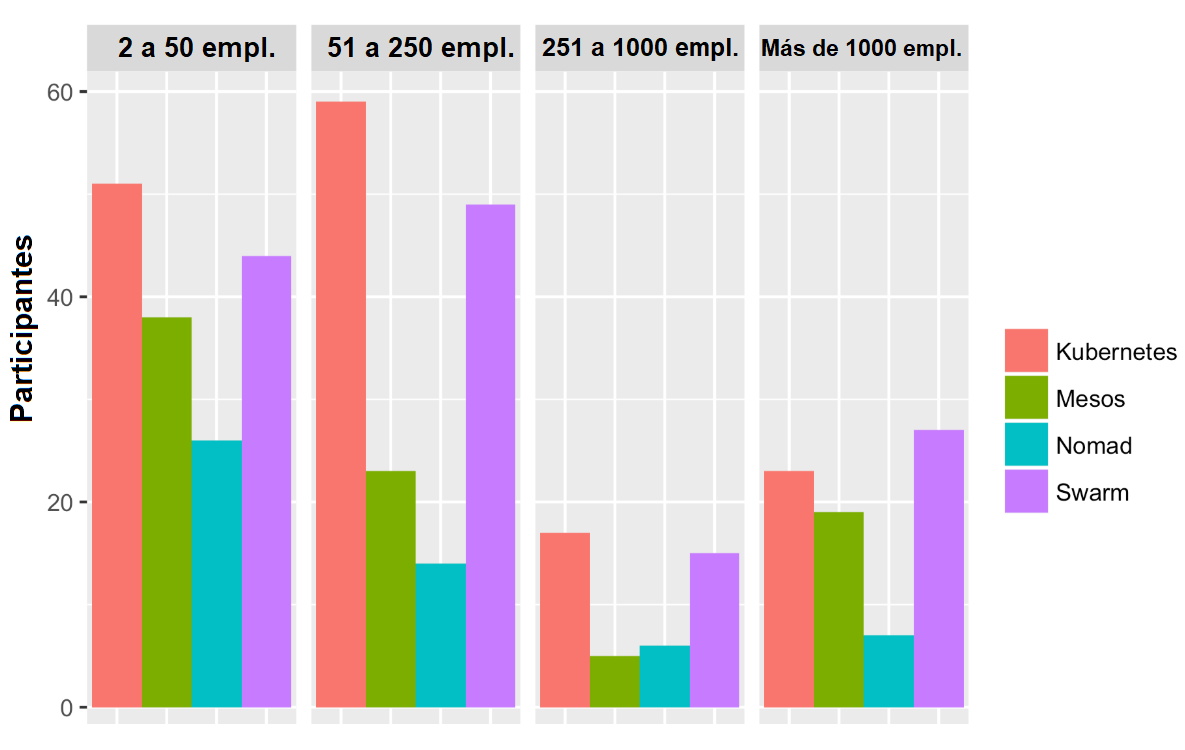
\includegraphics[scale=0.6]{Comparativa_Orquestadores_ES} 
\caption{Orquestadores utilizados por compañías según su tamaño (en número de empleados).}
\label{fig:Comparativa_Orquestadores_ES}
\end{figure}

\subsection{Revisión de trabajos realizados en la ETSInf}

En esta sección revisaremos diferentes trabajos de final de grado realizados por alumnos de la Escuela Técnica Superior de Ingeniería Informática (ETSInf). No son muchos los trabajos en la escuela relacionados con los microservicios debido a que su complejidad y a que estos son una tendencia muy actual. Queremos poner en valor dos trabajos, los realizados por Mompó \cite{Mompo2017} y Roig\cite{Roig2017}.

En el trabajo de Mompó se propone una nueva metodología de trabajo para disminuir el retrabajo e incrementar el código compartido en una organización. La memoria repasa prácticas como la integración continua, donde se comparan las herramientas de Jenkins y Bamboo. Esta nueva metodología incluye también el uso de una herramienta para integración continua. También realiza una comparativa entre una arquitectura basadas en microservicios y una monolítica frente a diferentes características como la escalabilidad o su complejidad. Entre las mayores diferencias que pueden observarse entre esta comparativa y la que realizamos en la sección \ref{sect:Comparativa} \nameref{sect:Comparativa} podemos citar la relacionada a la evolución de los microservicios. Según Mompó, introducir una modificación atañe solo al servicio al que se le aplica, cuando en este trabajo se presentan ejemplos de que esto no siempre es así.

En cuanto al trabajo de Roig, recoge en el estado del arte las principales características de los contenedores Docker y LXC. Sin embargo, muestra predilección por los segundos, cuando son los primeros los más adoptados en la industria.

\section{Propuesta} \label{sect:Propuesta}
%TODO Revisar

En el caso de estudio, en el desarrollo de la solución basada en microservicios se van a emplear contenedores Docker. Para su orquestación, en producción se hará uso de Kubernetes. En desarrollo, se hará uso de Docker Compose para agilizar la creación de los diferentes contenedores. 

En cuanto a la comunicación entre los servicios y con la interfaz de usuario, en la sección \ref{subsect:Integracion} \nameref{subsect:Integracion} hemos presentado tres posibles alternativas. Se ha optado por la que la literatura considera más sencilla, la integración REST a través de HTTP.

En cuanto a aspectos más técnicos, el lenguaje de programación que se va a emplear principalmente es C\# junto con el entorno de desarrollo (IDE) Visual Studio Enterprise 2017. Entre las plataformas de destino que ofrece la tecnología .NET vamos a utilizar tanto .NET Standard 2.0 como .NET Core en su versión 2.1, publicada en Mayo de 2018. \footnote{ Versiones de .NET Core 2.1: \url{https://www.microsoft.com/net/download/dotnet-core/2.1}} El uso de librerías distintas a las provistas por la plataforma se realizará a través de paquetes NuGet, un mecanismo sencillo que envuelve el código compilado de una librería y fácil de referenciar. \footnote{ Una introducción a NuGet: \url{https://docs.microsoft.com/es-es/nuget/what-is-nuget}}

Para el desarrollo de la interfaz de usuario se va a utilizar Xamarin.Forms. Xamarin es una plataforma que permite desarrollar aplicaciones móviles empleando código C\# para dispositivos Universal Windows Platform (UWP), Android y iOS. Xamarin.Forms es un conjunto de herramientas para Xamarin centrado en el desarrollo multiplataforma. Su propósito es que se pueda compartir la mayor cantidad de código posible en el desarrollo de una aplicación para las distintas plataformas que hemos mencionado. \footnote{ Introducción a Xamarin.Forms: \url{https://docs.microsoft.com/es-es/xamarin/xamarin-forms/get-started/introduction-to-xamarin-forms}}

A nivel de infraestructura se ha hecho uso de Microsoft Azure para la persistencia de datos en la nube y para la exposición de servicios a través de Azure App Service y Azure Kubernetes Service (AKS). Hemos decidido utilizar esta tecnología porque es la mejor soportada por el IDE en el que vamos a trabajar, ofreciendo funcionalidades para desplegar una nueva versión simplemente pulsando un botón. Tanto App Service como AKS son parte de los servicios de Azure. El primero se emplea para crear aplicaciones en la nube de forma rápida sin necesidad de administrar la infraestructura sobre la que se hospeda. En cuanto al segundo, permite la orquestación de contenedores Docker a través de Kubernetes dentro de la infraestructura de Azure. \footnote{ Página oficial de Microsoft Azure: \url{https://azure.microsoft.com/es-es/}}

Para terminar, para las pruebas a nivel de API se ha hecho uso de Postman. Postman es un entorno para el desarrollo de APIs (ADE) que nos va a permitir crear y almacenar de forma sencilla llamadas HTTP hacia la API del \textit{back-end}. \footnote{ Página oficial de Postman: \url{https://www.getpostman.com/}}

%%%%%%%%%%%%%%%%%%%%%%%%%%%%%%%%%%%%%%%%%%%%%%%%%%%%%%%%%%%%%%%%%%%%%%%%%%%%%%%
%                       Especificación de requisitos                                 %
%%%%%%%%%%%%%%%%%%%%%%%%%%%%%%%%%%%%%%%%%%%%%%%%%%%%%%%%%%%%%%%%%%%%%%%%%%%%%%%

\chapter{Especificación de requisitos del caso de estudio}

A continuación, presentaremos la descripción y especificación del caso de estudio. Los siguientes capítulos se enfocarán en la arquitectura de las soluciones y las tecnologías empleadas. Para centrarnos en esto, en lugar de pensar en un dominio de negocio hipotético que quizás no conozca, hemos seleccionado un dominio de negocio bien conocido. En concreto, una aplicación simplificada de comercio electrónico (\textit{e-shop}) para la toma de pedidos y la gestión de incidencias.

\section{Descripción del caso de estudio}

Se desea desarrollar un sistema para la venta de productos electrónicos a través de dispositivos móviles. La aplicación móvil estará destinada solo a los clientes de una tienda, que deberán registrarse para usarla.

Los clientes podrán consultar los \textbf{productos} disponibles en la tienda junto con su precio, descripción y número de unidades en stock. Un \textbf{pedido} se define como un conjunto de productos que el cliente ha seleccionado junto con el número de unidades de cada uno. Mientras no se haya confirmado el pedido, se podrán añadir y eliminar productos al pedido en elaboración.

Todos los pedidos realizados por un cliente se mostrarán en un listado junto con el estado de los mismos. Para cada pedido, el cliente podrá generar una \textbf{factura} donde se listan los productos que lo componen y el precio total.

Una vez un cliente haya confirmado un pedido, este deberá ser aprobado por un empleado para ser entregado. Cuando esto suceda, se enviará una \textbf{notificación} al correo electrónico del cliente. Mientras que el empleado no lo apruebe, el pedido podrá ser cancelado. Además, cuando el pedido sea entregado físicamente al cliente, este deberá marcar el pedido como entregado.

Un cliente puede crear una \textbf{incidencia} si tiene algún problema con un pedido o quiere consultar una duda con los empleados de la tienda. Dentro de una incidencia, tanto el cliente como los empleados se comunicarán a través de \textbf{comentarios}. Cuando lo considere oportuno, el cliente podrá cerrar la incidencia creada, que podrá volver a consultar en cualquier momento.

A partir de la descripción del sistema podemos definir el siguiente modelo de dominio:

\begin{figure}[h]
\centering
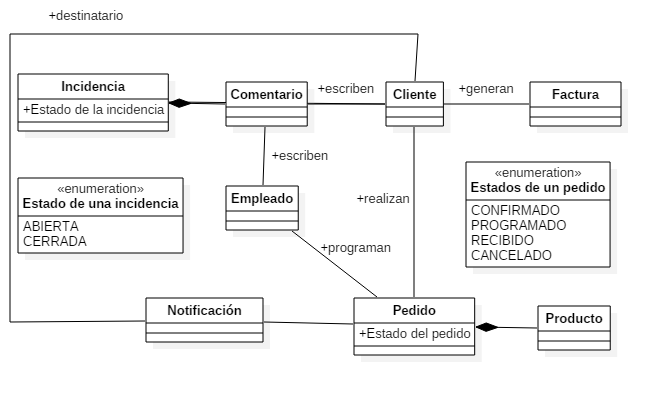
\includegraphics[scale=0.5]{modelo_dominio_final}
\caption{Modelo de dominio del sistema.}
\end{figure}

\section{Casos de uso} \label{sect:CUs}

A continuación, vamos a listar los casos de uso de la aplicación móvil. En los casos de uso aumentaremos el nivel de detalle de la descripción para emplearlos como especificación del sistema. El único usuario de la aplicación móvil es el cliente de la tienda, por lo que es el actor de todos los casos citados. Para cada caso de uso se va a proveer un identificador, un título y una descripción breve:

\begin{center}
\begin{tabular}{ | c | l | }
\hline
\textbf{ CU001 } & Iniciar sesión en la aplicación \\
\hline
\multicolumn{2}{ | p{14cm} | }
{
Para iniciar sesión, el usuario debe haberse registrado previamente en la aplicación. Para hacerlo debe proveer simplemente su correo electrónico y su contraseña.
} \\
\hline
\end{tabular}
\end{center}

\begin{center}
\begin{tabular}{ | c | l | }
\hline
\textbf{ CU002 } & Registrarse en la aplicación \\
\hline
\multicolumn{2}{ | p{14cm} | }
{
Cualquier persona que tenga la aplicación instalada en su dispositivo móvil puede registrarse como cliente. Para hacerlo, simplemente ha de proveer su nombre, su correo electrónico y una contraseña.
} \\
\hline
\end{tabular}
\end{center}

\begin{center}
\begin{tabular}{ | c | l | }
\hline
\textbf{ CU003 } & Listar los productos de la tienda \\
\hline
\multicolumn{2}{ | p{14cm} | }
{
El cliente puede consultar todos los productos disponibles en la tienda. Para cada producto se mostrará una imagen, el nombre del producto y su precio. El usuario podrá buscar un producto por su nombre y ordenar el listado por nombre y precio.
} \\
\hline
\end{tabular}
\end{center}

\begin{center}
\begin{tabular}{ | c | l | }
\hline
\textbf{ CU004 } & Visualizar un producto \\
\hline
\multicolumn{2}{ | p{14cm} | }
{
El cliente puede ver la descripción de un producto, su precio y número de unidades en stock. Cuando lo desee, el usuario puede seleccionarlo para comprarlo y crear así un nuevo pedido.
} \\
\hline
\end{tabular}
\end{center}

\begin{center}
\begin{tabular}{ | c | l | }
\hline
\textbf{ CU005 } & Crear un pedido \\
\hline
\multicolumn{2}{ | p{14cm} | }
{
El cliente puede crear un pedido y añadir en él productos. Para cada uno, debe especificar el número de unidades que desea. En cualquier momento puede eliminar cualquiera de los productos que componen el pedido. Cuando lo considere oportuno, el cliente ha de confirmar el pedido que está creando para que sea tramitado.
} \\
\hline
\end{tabular}
\end{center}

\begin{center}
\begin{tabular}{ | c | l | }
\hline
\textbf{ CU006 } & Cancelar un pedido \\
\hline
\multicolumn{2}{ | p{14cm} | }
{
Para los pedidos confirmados, mientras estos no hayan sido gestionados por un empleado para su entrega, el pedido se podrá cancelar.
} \\
\hline
\end{tabular}
\end{center}

\begin{center}
\begin{tabular}{ | c | l | }
\hline
\textbf{ CU007 } & Generar factura de un pedido \\
\hline
\multicolumn{2}{ | p{14cm} | }
{
El cliente podrá generar una factura para cualquiera de sus pedidos. La factura se generará en formato PDF e incluirá la siguiente información: los datos del cliente, el listado de todos los productos que componen el pedido junto con su precio unitario y el precio total del pedido antes y después de aplicar el IVA.
} \\
\hline
\end{tabular}
\end{center}

\begin{center}
\begin{tabular}{ | c | l | }
\hline
\textbf{ CU008 } & Marcar un pedido como recibido \\
\hline
\multicolumn{2}{ | p{14cm} | }
{
Cuando un pedido se entregue físicamente a un cliente, este deberá marcar a través de la aplicación el pedido como recibido.
} \\
\hline
\end{tabular}
\end{center}

\begin{center}
\begin{tabular}{ | c | l | }
\hline
\textbf{ CU009 } & Listar los pedidos del cliente \\
\hline
\multicolumn{2}{ | p{14cm} | }
{
Todos los pedidos que ha realizado un cliente se podrán listar en cualquier momento, mostrando la fecha en que se realizó y su estado actual. Los pedidos aparecen ordenados por la fecha en la que se realizaron. El listado se puede filtrar por el estado de los pedidos. Los posibles estados de un pedido son: CONFIRMADO, PROGRAMADO, RECIBIDO y CANCELADO.
} \\
\hline
\end{tabular}
\end{center}

\begin{center}
\begin{tabular}{ | c | l | }
\hline
\textbf{ CU010 } & Crear una incidencia \\
\hline
\multicolumn{2}{ | p{14cm} | }
{
Un cliente puede crear una incidencia si tiene algún problema con un pedido o quiere consultar una duda con los empleados de la tienda. Para hacerlo, ha de proveer un título que describa el problema o consulta.
} \\
\hline
\end{tabular}
\end{center}

\begin{center}
\begin{tabular}{ | c | l | }
\hline
\textbf{ CU011 } & Añadir un comentario en una incidencia \\
\hline
\multicolumn{2}{ | p{14cm} | }
{
En el contexto de una incidencia, los clientes podrán comunicarse a través de comentarios con los empleados de la tienda. En la incidencia se verán los comentarios tanto de los empleados como del cliente ordenados cronológicamente. Para cada comentario se mostrará el nombre del autor, la fecha en la que lo escribió y el contenido del mismo.
} \\
\hline
\end{tabular}
\end{center}

\begin{center}
\begin{tabular}{ | c | l | }
\hline
\textbf{ CU012 } & Cerrar una incidencia \\
\hline
\multicolumn{2}{ | p{14cm} | }
{
Solo el cliente puede cerrar una incidencia que haya abierto. Cuando lo haga, el cliente podrá seguir accediendo a ella pero ya no podrá añadir nuevos comentarios. Tampoco le estará permitido volver a abrirla.
} \\
\hline
\end{tabular}
\end{center}

\begin{center}
\begin{tabular}{ | c | l | }
\hline
\textbf{ CU013 } & Listar las incidencias del cliente \\
\hline
\multicolumn{2}{ | p{14cm} | }
{
Se pueden consultar todas las incidencias creadas por el cliente en un listado donde se mostrará tanto la fecha en la que se crearon como su estado actual. El listado aparecerá ordenado por la fecha de creación de las incidencias y se podrá filtrar por el estado de las mismas. Los posibles estados de las incidencias son: ABIERTA y CERRADA.
} \\
\hline
\end{tabular}
\end{center}

%%%%%%%%%%%%%%%%%%%%%%%%%%%%%%%%%%%%%%%%%%%%%%%%%%%%%%%%%%%%%%%%%%%%%%%%%%%%%%%
%                       Proceso de desarrollo
%
%%%%%%%%%%%%%%%%%%%%%%%%%%%%%%%%%%%%%%%%%%%%%%%%%%%%%%%%%%%%%%%%%%%%%%%%%%%%%%%

\chapter{Proceso de desarrollo}

\section{Plan de trabajo} \label{sct:PlanTrabajo}

El sistema a implementar se puede dividir en dos partes: \textit{front-end} y \textit{back-end}. En lo referente al \textit{back-end}, este se va a implementar siguiendo dos arquitecturas distintas: una monolítica y otra basada en microservicios. Existirá una gran cantidad de código compartido entre ambas soluciones y las mayores diferencias entre ellas serán las relacionadas con la organización del código. Por este motivo, primero se va a implementar la solución monolítica y una vez implementada se creará una nueva solución donde se refactorizará el código para obtener la solución basada en microservicios, siguiendo los principios que en la sección \ref{sct:FaseDiseño} \nameref{sct:FaseDiseño} se han mencionado.

Una vez se implemente la solución monolítica, se comenzará la implementación de la aplicación front-end. Las llamadas a la parte servidora van a realizarse a través de invocaciones HTTP. En consecuencia, el \textit{front-end} va a estar desacoplado de la implementación que elijamos para el \textit{back-end} y va a poder emplearse la misma solución, con muy pequeñas modificaciones, para comunicarse con ambas partes servidoras.

La organización de la memoria en los siguientes capítulos es acorde a este proceso. Primero, presentaremos la solución monolítica centrándonos sobre todo en aspectos de implementación, que son comunes a los de la solución basada en servicios. Después, explicaremos la solución basada en microservicios, centrándonos sobre todo en aspectos de diseño y modificaciones que se han realizado frente a la monolítica.

\section{Organización del trabajo}

El proceso de desarrollo se ha desglosado en grandes tareas, muy ligadas a las entidades del dominio que existen en el caso de estudio. En el siguiente cronograma mostrado en la figura \ref{fig:Cronograma} se pueden observar estas tareas y su evolución a lo largo del tiempo que ha durado el desarrollo de las soluciones. En azul se han representado las tareas asociadas a la solución monolítica, en verde las asociadas al front-end y en naranja las asociadas a la solución basada en microservicios.

\begin{figure}[h]
\centering
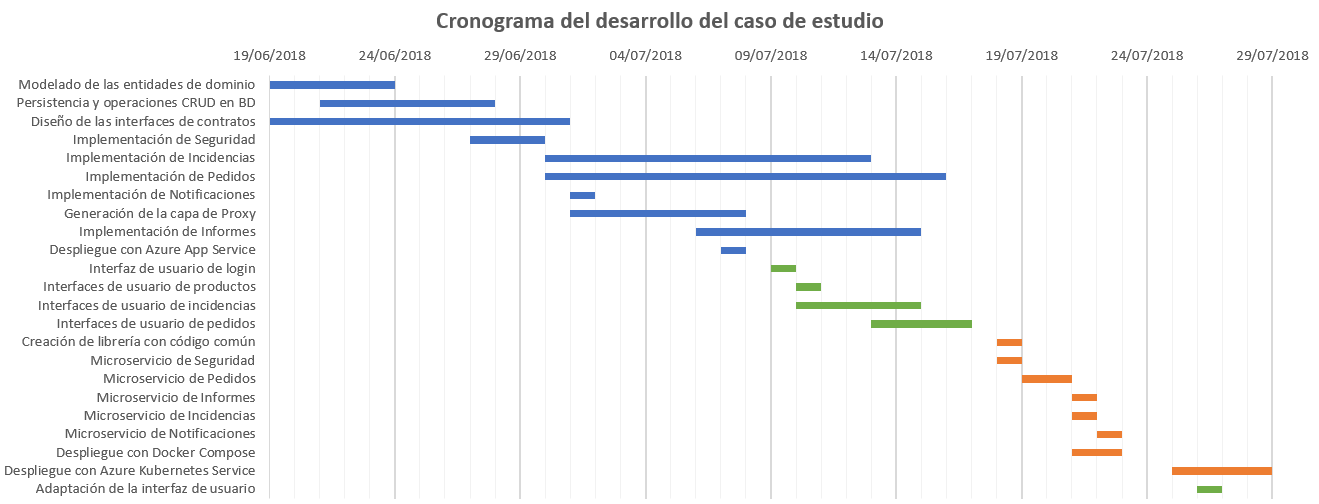
\includegraphics[scale=0.5]{Cronograma}
\caption{Cronograma del proceso de desarrollo del caso de estudio.}
\label{fig:Cronograma}
\end{figure}

Se puede observar como de las tres actividades del desarrollo donde más esfuerzo se ha dedicado es en la implementación de la solución monolítica. Esto es porque es aquí donde se ha implementado casi la totalidad del código del sistema y donde se han evaluado muchas de las tecnologías empleadas. La fase de desarrollo de la solución basada en microservicios se prolonga menos porque únicamente ha involucrado refactorizar el diseño monolítico y a penas se ha modificado la implementación del sistema. En un sistema real, esta tarea sería mucho más costosa que en nuestro caso de estudio.

Todo el código desarrollado se va a almacenar en un repositorio de código de GitHub. Se han creado tres repositorios: uno para el \textit{back-end} monolítico, otro para la interfaz de usuario y otro para el \textit{back-end} basado en servicios. Adicionalmente, se ha creado un repositorio para el desarrollo de la memoria de este TFG.

En los repositorios de GitHub vamos a emplear un proyecto. Un proyecto de GitHub es similar a un Trello. Aquí podemos crear columnas, que representan un estado del trabajo, y tarjetas, que representan tareas a realizar y que van transitando de una columna a otra conforme se van completando. En nuestro caso, las tareas que vamos a incluir en el proyecto son de un detalle más bajo a las que hemos incluido en el cronograma, más cercanas a las tareas que debe llevar a cabo el programador. El proyecto lo hemos dividido en 4 columnas: TODO, que contiene las tareas pendientes, TODO - Priority, que contiene también tareas pendientes pero que urge resolver, DONE, para las tareas ya realizadas, y DISCARD, para las tareas que se han descartado y ya no se van a implementar. La figura \ref{fig:GitHubProject} ilustra estas columnas para el proyecto de la aplicación móvil en un estado casi final de su desarrollo.

\begin{figure}[h]
\centering
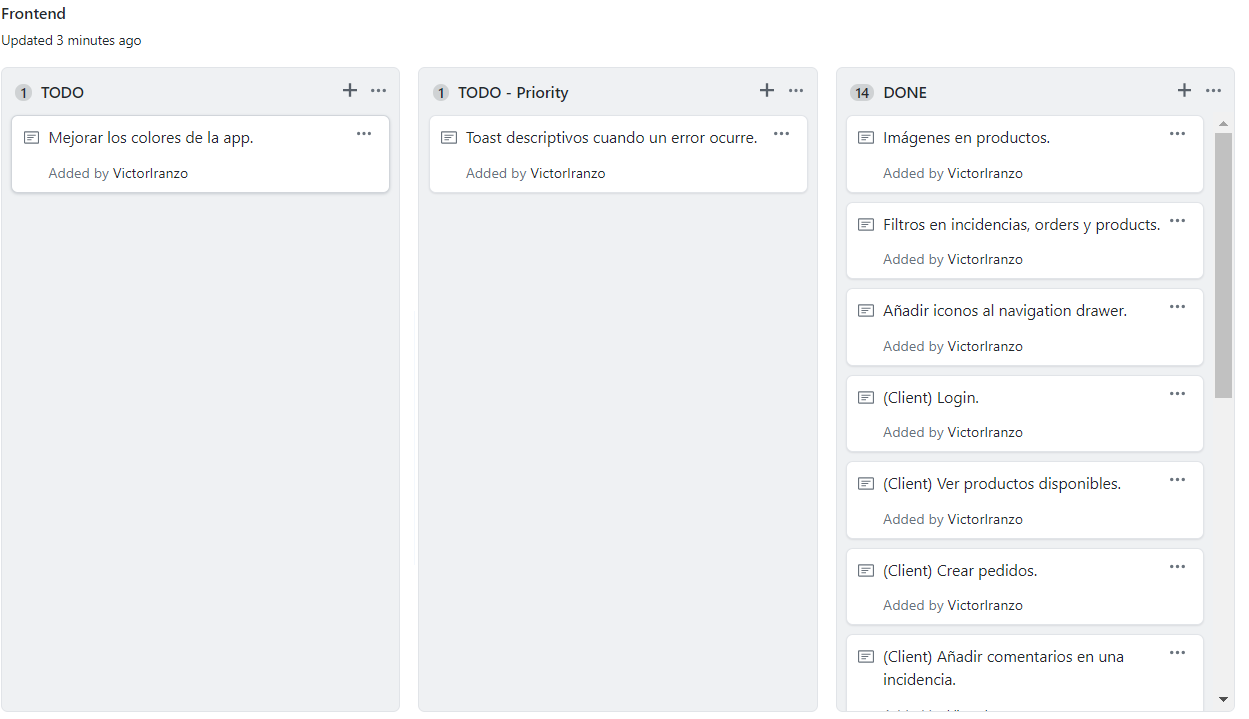
\includegraphics[scale=0.6]{GitHubProject}
\caption{Proyecto de GitHub asociado al desarrollo del \textit{front-end}.}
\label{fig:GitHubProject}
\end{figure}

%%%%%%%%%%%%%%%%%%%%%%%%%%%
% SALTO DE PAGINA
%%%%%%%%%%%%%%%%%%%%%%%%%%%
\newpage


El proceso de desarrollo se puede visualizar en los diferentes repositorios a través de los \textit{commits} (la unidad de los repositorios de código git que representa los cambios que se guardan en el repositorio) realizados. En el siguiente gráfico se muestra el número de \textit{commits} realizados cada día sobre los tres repositorios mencionados. Como en el cronograma, se puede ver como los períodos de \textit{front-end} e implementación de la solución monolítica se superponen en la mitad del proceso de desarrollo. También se puede ver como la fase de la solución monolítica es la que más \textit{commits} ha requerido porque ha sido la más inestable respecto a defectos corregidos y detalles de implementación.

\begin{figure}[h]
\centering
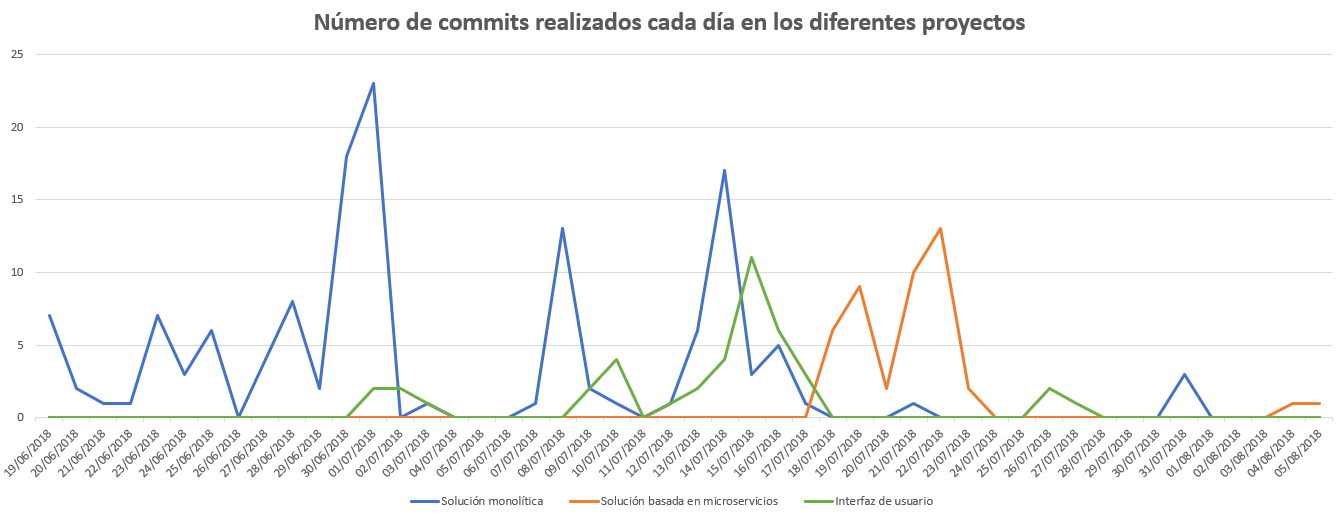
\includegraphics[scale=0.5]{commits}
\caption{Número de \textit{commits} realizados cada día en los repositorios del caso de estudio.}
\end{figure}

%%%%%%%%%%%%%%%%%%%%%%%%%%%%%%%%%%%%%%%%%%%%%%%%%%%%%%%%%%%%%%%%%%%%%%%%%%%%%%%
%                       MONOLITICA
%
%%%%%%%%%%%%%%%%%%%%%%%%%%%%%%%%%%%%%%%%%%%%%%%%%%%%%%%%%%%%%%%%%%%%%%%%%%%%%%%

\chapter{Diseño e implementación de la solución monolítica}

\section{Diseño de la solución} \label{sct:DiseñoMonolitico}

A nivel arquitectónico, la aplicación monolítica va a seguir una arquitectura de 6 capas, que es la que se emplea en la empresa donde el autor trabaja actualmente. Detallamos a continuación sus detalles:

\begin{itemize}

\item \textbf{Capa de contratos}: en esta capa se situarán las interfaces que contienen todas las acciones del \textit{back-end} que pueden ser invocadas desde el exterior a través de la API. Estas interfaces se implementarán tanto en las capas de aplicación, servicios y proxy. 

También se situarán en esta capa los objetos para la transferencia de datos (DTO). Los DTOs se utilizan para desacoplar los servicios que ofrece una API de la representación interna que da el sistema a sus entidades. En lugar de devolver al cliente una entidad tal y como se almacena en base de datos, los DTOs representan una entidad ocultando aquellas propiedades que no necesitan ser transferidas. También pueden cambiar el formato de algunas propiedades para que sea más cómodo para el cliente su procesamiento. \footnote{ Crear objetos de transferencia de datos (DTO): \url{https://docs.microsoft.com/es-es/aspnet/web-api/overview/data/using-web-api-with-entity-framework/part-5}}

\item \textbf{Capa de aplicación}: en esta capa es donde se implementa la lógica de la parte servidora. Aquí se da implementación a las interfaces que se sitúan en la capa de contratos. Es en esta capa donde se validan los permisos de un usuario que ha realizado una petición al servidor sobre la acción que desea realizar. En caso de que se trate de hacer una operación no válida será esta capa la encarga de lanzar la excepción oportuna. También aquí se situarán los conversores para transformar una entididad en un DTO, que se emplearán principalmente en las operaciones CRUD.

\item \textbf{Capa de servicios}: contiene el punto de entrada del proceso que representa al \textit{back-end} (el método Main). En esta capa se encuentran los controladores, donde se definen todas las acciones de la API. Cada acción se define a través de un verbo HTTP, la URL donde se localiza y sus parámetros, que pueden ser obtenidos a partir del cuerpo o la cabecera de una petición. La capa de servicios delega en la capa de aplicación para devolver un resultado a cada una de las peticiones que atiende. \footnote{ Control de solicitudes con controladores en ASP.NET Core MVC: \url{https://docs.microsoft.com/es-ES/aspnet/core/mvc/controllers/actions?view=aspnetcore-2.1}}

\item \textbf{Capa de dominio}: contiene las entidades del dominio del sistema junto con sus propiedades y los estados asociados a estas. Esta capa es referenciada tanto por la capa de aplicación como por la capa de persistencia.

\item \textbf{Capa de persistencia}: la capa de persistencia ofrece operaciones CRUD para cada una de las entidades que se almacenan en BD a través objetos para el acceso a datos (DAO). La capa de persistencia no trabaja con DTOs: cuando la capa de aplicación le solicita una entidad, la devuelve completa. Es la capa de aplicación quien a través de los conversores transforma la entidad en un DTO para devolver una representación de esta al usuario.

\item \textbf{Capa de proxy}: esta capa contiene los clientes necesarios para invocar al \textit{back-end} a través de llamadas HTTP realizadas por código C\#. Esta capa será referenciada por el \textit{front-end} a través de un paquete NuGet para comunicar con el \textit{back-end}. El \textit{front-end} es quien ejecutará el código contenido en esta capa. Cuando se desee comunicar con la parte servidor, en el proceso del \textit{front-end} se invocará al proxy para realizar una llamada HTTP al \textit{back-end}. Como debe ofrecer todas las operaciones de la API, implementa las interfaces de la capa de contratos.

\end{itemize}

\begin{figure}[h]
\centering
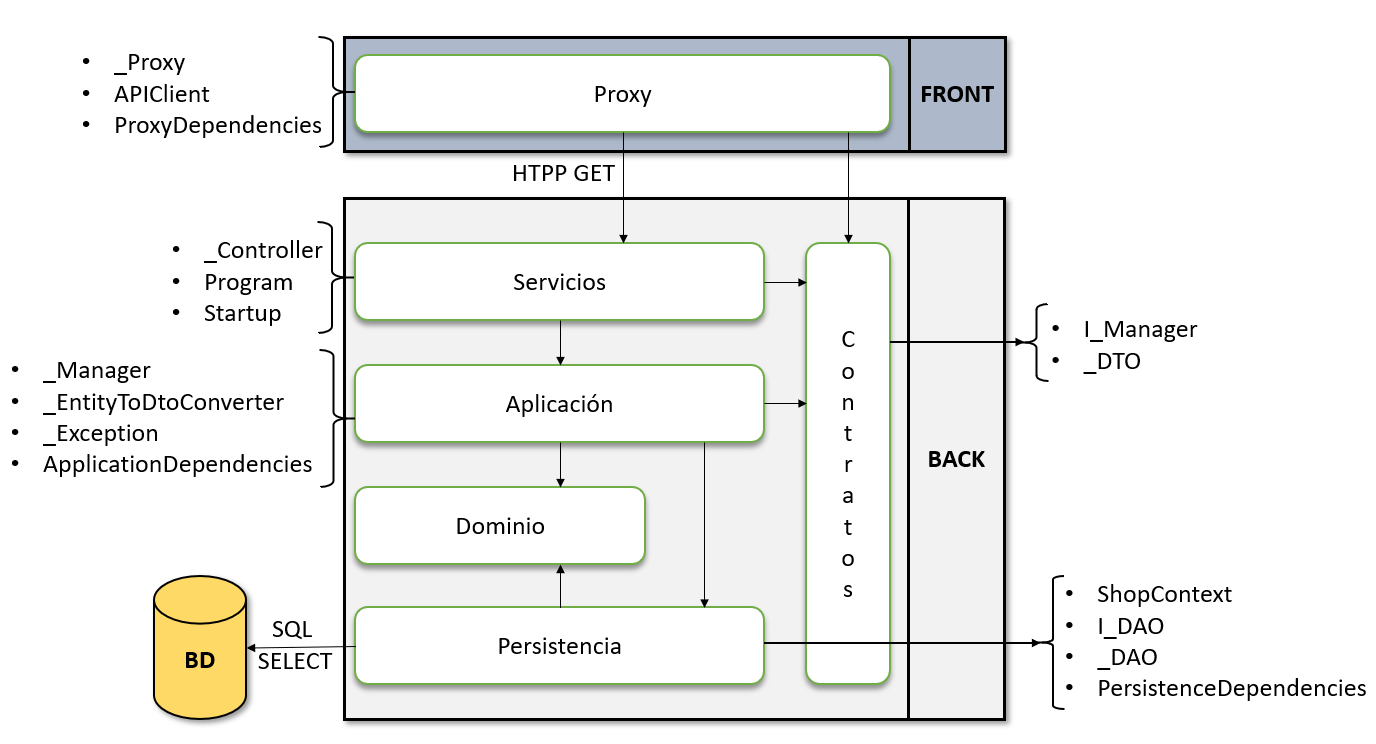
\includegraphics[scale=0.5]{capas}
\caption{Capas del back-end monolítico.}
\label{fig:capas}
\end{figure}

En la figura \ref{fig:capas} se representa la arquitectura de 6 capas. Mediante flechas se señala que una capa depende de otra. También se ha representado la base de datos, a la que solo se accede desde la capa de persistencia. De cada capa se ha especificado el estándar usado para nombrar de las clases más importantes en el código. Por ejemplo, de la capa de aplicación se señala \textit{\_Manager}; los \textit{managers} serán las clases donde se implemente la lógica para cada una de las entidades del dominio, dando lugar a clases como \textit{ProductsManager} o \textit{IncidencesManager}. Lo mismo ocurre con el patrón \textit{I\_DAO} en la persistencia, que define una interfaz para el acceso a datos de una entidad y que da lugar a clases como \textit{IOrdersDAO}.

A nivel de la solución en Visual Studio, cada capa consistirá en un proyecto distinto, tal como se muestra en la figura \ref{fig:MonolithicSolution}. Un proyecto consiste en un archivo XML con extensión *.csproj que tiene una plataforma y dependencias específicas y que se puede compilar de forma independiente. Cada proyecto es un contenedor que organiza sus clases y otros archivos de forma jerárquica. \footnote{ Soluciones y proyectos en Visual Studio: \url{https://docs.microsoft.com/es-es/visualstudio/ide/solutions-and-projects-in-visual-studio}} Adicionalmente, existe un proyecto que contiene las pruebas del sistema. Todos los proyectos son .NET Standard 2.0 salvo los de las capa de servicios y pruebas, cuya plataforma es .NET Core 2.1 porque no son librerías y pueden ser ejecutados.

\begin{figure}[h]
\centering
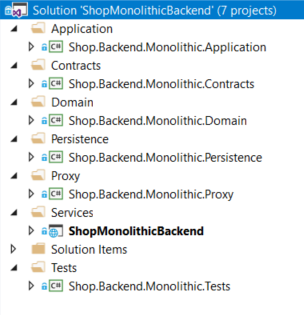
\includegraphics[scale=0.8]{MonolithicSolution}
\caption{Solución del sistema monolítico.}
\label{fig:MonolithicSolution}
\end{figure}

A nivel de diseño, se van a definir las siguientes entidades en la capa de dominio: pedido (\textit{Order}), producto (\textit{Product}), compra (\textit{Purchase}), incidencia (\textit{Incidence}) y comentario (\textit{Comment}). Estas entidades se pueden obtener a partir del modelo de dominio. Sin embargo, algunos conceptos que aparecen en el modelo de dominio como los informes o las notificaciones no vamos a modelarlas como entidades. No son entidades como tal porque no necesitamos almacenarlas o ofrecer operaciones CRUD sobre ellas, así que vamos a modelarlas como acciones. Simplemente ofreceremos métodos para generar un informe (\textit{GenerateReport}) y enviar notificaciones (\textit{SendNotification}).

Cabe destacar en el diseño la relación que existe entre un pedido y un producto. Esta relación es de muchos a muchos: un pedido está formado por múltiples productos y un producto puede estar incluido en diferentes pedidos. Además, la relación cuenta con una propiedad que es el número de unidades del producto en el pedido, que se puede modelar como un atributo en una clase asociación. Si razonamos a nivel de base de datos, la clase asociación se implementará como una tabla intermedia entre las tablas de pedidos y productos. En nuestro código, también lo modelaremos así, dando lugar a la entidad intermedia \textit{Purchase}. Esto lo hacemos para hacer uso de la librería Entity Framework en el mapeo objeto-relacional (ORM), que nos facilitará el acceso a la base de datos.

Con todo esto, el diagrama de clases que se encuentran en la capa de dominio será el que se ilustra en la siguiente figura. En esta figura ya se ilustran las propiedades de las entidades de dominio.

\begin{figure}[h]
\centering
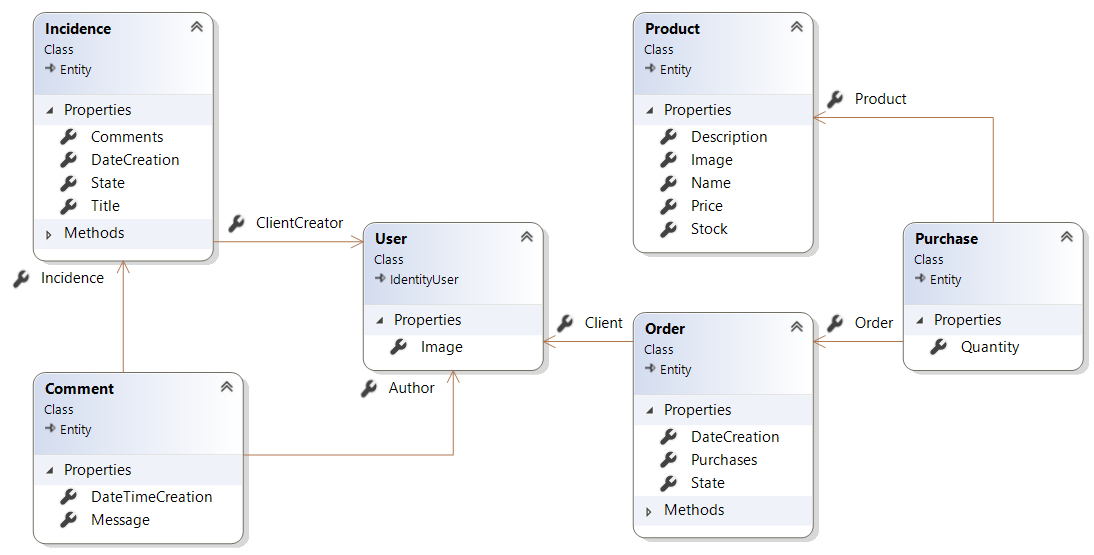
\includegraphics[scale=0.65]{ClassDiagram}
\caption{Diagrama de clases de dominio de la solución monolítica.}
\end{figure}

%%%%%%%%%%%%%%%%%%%%%%%%%%%
% SALTO DE PAGINA
%%%%%%%%%%%%%%%%%%%%%%%%%%%
\newpage

\section{Detalles de la implementación back-end}

\subsection{Operaciones CRUD} \label{subsect:CRUD}

Para la mayoría de entidades que hemos modelado vamos a ofrecer operaciones CRUD. Esto se hará a través de las interfaces que expone la parte servidora en la capa de contratos (\textit{IOrdersManager} o \textit{ICommentsManager} son algunos ejemplos). Con este propósito, vamos a definir una interfaz genérica que exponga estas operaciones de forma unitaria y agregada. En los servicios, las operaciones agregadas son un mecanismo para evitar que dos componentes tengan que comunicarse continuamente. Si se tienen que crear una colección de entidades, en lugar de crear una petición al servidor para cada entidad, se envía una única petición con toda la colección \cite{Newman2015a}.

\begin{figure}[h]
\centering
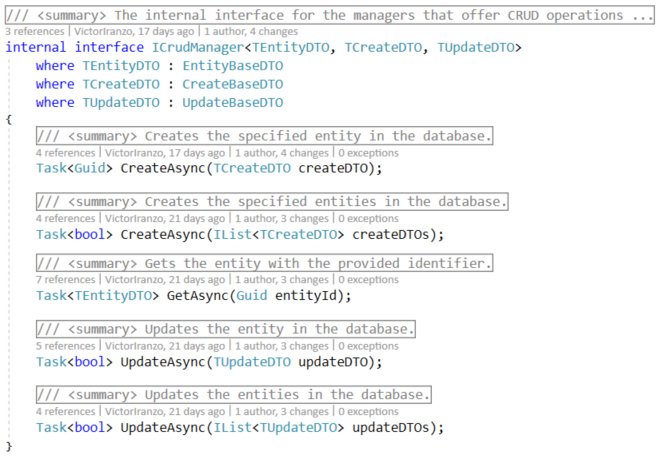
\includegraphics[scale=0.8]{ICrudManager}
\caption{Interfaz interna para las operaciones CRUD.}
\label{fig:ICrudManager}
\end{figure}

En la figura \ref{fig:ICrudManager} se muestra la interfaz genérica que hemos mencionado. La interfaz \textit{ICrudManager} es interna porque no debe ser visible fuera de la solución del back-end. Es genérica porque se define en base a DTOs con diferentes propósitos. Para la creación de una entidad son necesarias solo algunas propiedades y otras como la fecha de creación son calculadas por el sistema y no deben ser provistas en el \textbf{\textit{CreateDTO}} de la petición. Lo mismo ocurre con la lectura y la actualización de una entidad. Por ejemplo, de una entidad algunas propiedades no está permitido actualizarlas, por lo que no deben incluirse estas en el \textbf{\textit{UpdateDTO}} de la entidad. 

Sin embargo, no se van a definir únicamente operaciones CRUD para una entidad. Cada entidad tiene una serie de operaciones asociadas, como puede ser generar la factura de un pedido o obtener la lista de incidencias de un usuario. Tanto estas acciones como las CRUD se definen en la interfaz de contratos de la entidad. Si para una entidad se quieren exponer operaciones CRUD, se deben definir los DTOs específicos para las operaciones de lectura, escritura y actualización y se debe extender la interfaz genérica. 

En la interfaz de la figura \ref{fig:IOrdersManager} se observa la interfaz de contratos de la entidad pedido, que extiende la interfaz genérica \textit{ICrudManager} con los DTOs \textit{OrderDTO}, \textit{OrderCreateDTO} y \textit{OrderUpdateDTO}. Por ejemplo, \textit{OrderUpdateDTO} no cuenta con ningún atributo que represente la fecha en la que se creó el pedido porque esta propiedad de la entidad no puede ser modificada. También se puede observar el método definido para la generación de una factura, \textit{GenerateOrderReportAsync}.

\begin{figure}[h]
\centering
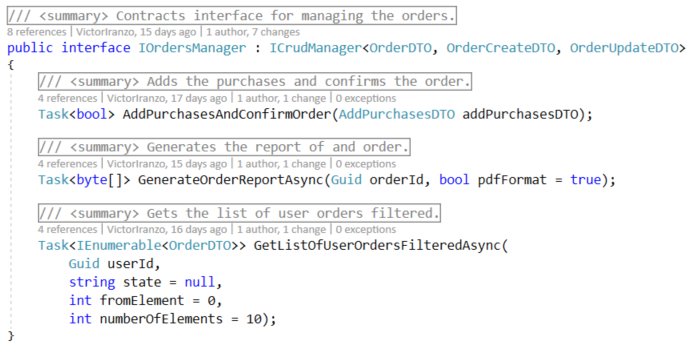
\includegraphics[scale=0.8]{IOrdersManager}
\caption{Interfaz en la capa de contratos asociada a la entidad Pedido.}
\label{fig:IOrdersManager}
\end{figure}

La implementación de las operaciones CRUD en la capa de aplicación también se realizará de forma genérica, a través de la clase llamada \textit{CrudManager}. Si la implementación de una de las operaciones no se ajusta a la que una entidad necesita, esta puede ser sobreescrita en el \textit{manager} de la entidad.

Por último, algunas entidades en lugar de ofrecer operaciones CRUD solo ofrecen \textbf{operaciones CUD} (crear, actualizar y eliminar). Estas entidades son las de Comentario y Compra porque podemos considerarlas como secundarias. No tiene sentido exponer un método en la interfaz de \textit{back-end} para leer un único comentario o obtener el número de unidades de un producto en un pedido. No obstante, si que tiene sentido exponer un método para, por ejemplo, crear o eliminar un comentario dentro de una incidencia. Las operaciones de lectura de estas entidades se realizan a través de su entidad principal asociada. Por ejemplo, cuando solicitamos una incidencia obtendremos todos los comentarios que en la incidencia se han hecho aunque los comentarios sean objetos de una entidad independiente.

\subsection{Seguridad}
%TODO Ha faltado mencionar registro en la clase PersistenceDependencies.
% https://auth0.com/blog/securing-asp-dot-net-core-2-applications-with-jwts/
% https://docs.microsoft.com/es-es/aspnet/core/security/authorization/roles?view=aspnetcore-2.1
% https://docs.microsoft.com/es-es/aspnet/core/security/authorization/simple?view=aspnetcore-2.1
% https://docs.microsoft.com/es-es/aspnet/core/security/authentication/identity?view=aspnetcore-2.1&tabs=visual-studio%2Caspnetcore2x

La mayoría de métodos expuestos en la API del \textit{back-end} requieren de mecanismos de autorización para establecer si la persona que realiza una petición puede acceder o no a los datos que solicita. Con este propósito, vamos a hacer uso de \textbf{ASP.NET Core Identity} y de \textit{tokens} de seguridad JWT (JSON Web Token). 

Identity es el sistema de ASP.NET Core para administrar los usuarios registrados de una aplicación a través de proveedores externos como Google y Facebook o a través de una base de datos de usuarios propia. \footnote{ Introducción a la identidad en ASP.NET Core: \url{https://docs.microsoft.com/es-es/aspnet/core/security/authentication/identity}} Atendiendo a los requisitos especificados, no necesitamos que nuestros usuarios se puedan autenticar a través de proveedores externos, por lo que vamos a optar por gestionar los usuarios de la aplicación nosotros mismos. Los pasos para conseguirlo se resumen a continuación:

\begin{itemize}

\item En la capa de dominio, se debe crear una entidad que represente al usuario de la aplicación y que herede de la clase \textit{IdentityUser}. La clase \textit{IdentityUser} provee numerosos atributos, como el nombre o el correo electrónico.

\item En la capa de persistencia, para asegurar la creación de las tablas asociadas a Identity, el contexto de la aplicación que representa a la BD debe extender la clase \textit{IdentityDbContext<User>}. En la base de datos, las tablas de datos creadas automáticamente por Identity se identifican por el prefijo AspNet. En la figura \ref{fig:BDMonolitica} se muestra la BD de la solución monolítica, resaltando las tablas asociadas a Identity.

\begin{figure}[h]
\centering
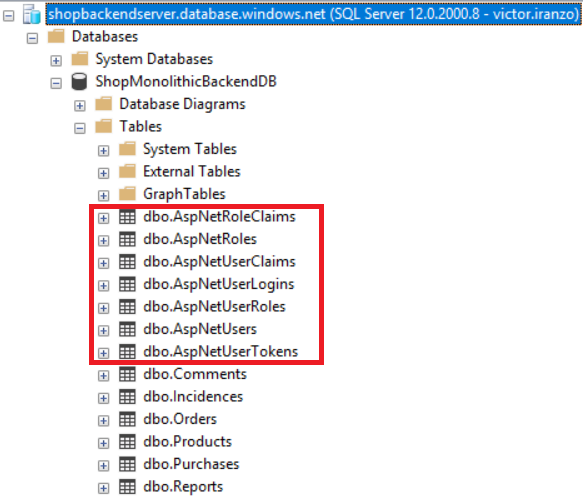
\includegraphics[scale=0.8]{BDMonolitica}
\caption{Tablas creadas por ASP.NET Core Identity.}
\label{fig:BDMonolitica}
\end{figure}

\item En la capa de servicios, a los métodos de la API que requieran de autorización se les ha de añadir el atributo \textit{Authorize}. Con esto, cuando se realice una petición sin proveer un \textit{token} de autorización se devolverá automáticamente un error 401: Unauthorized. En el atributo \textit{Authorize} se puede especificar si el método puede ser ejecutado solo por los usuarios que tengan cierto rol. \footnote{ Autorización basada en roles en ASP.NET Core: \url{https://docs.microsoft.com/es-es/aspnet/core/security/authorization/roles?view=aspnetcore-2.1}} Por ejemplo, podemos establecer que las operaciones agregadas de tipo CRUD solo puedan ser invocadas por los usuarios con el rol Administrador, como muestra la figura \ref{fig:Authorize}.

\begin{figure}[h]
\centering
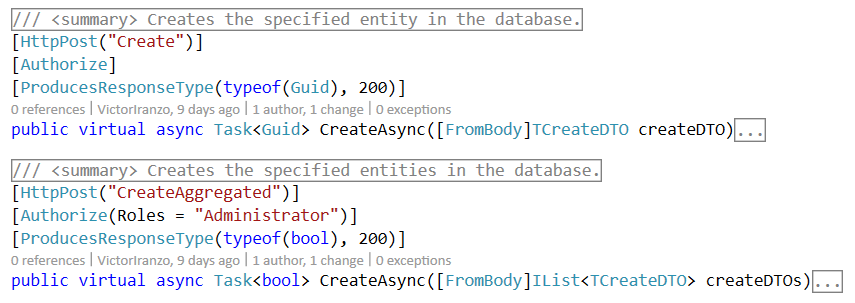
\includegraphics[scale=0.7]{Authorize}
\caption{Ejemplo de métodos de la clase de servicios.}
\label{fig:Authorize}
\end{figure}

\end{itemize}

El usuario podrá obtener el \textit{token} que le identifica a través del método \textit{Login} del \textit{manager} de Seguridad. Para hacerlo, deberá proveer su correo electrónico y contraseña. En la implementación de este método en la capa de aplicación se comprueba que el correo electrónico y contraseña coinciden con los almacenados en las tablas de Identity. Si coinciden, el método devuelve un \textit{token} JWT donde se incluirán los datos del usuario y la fecha en la que el \textit{token} expira. En cada petición HTTP que haga el usuario a la parte servidora deberá proveer este en la cabecera, como muestra el ejemplo de la figura \ref{fig:http}.

\begin{figure}[h]
\centering
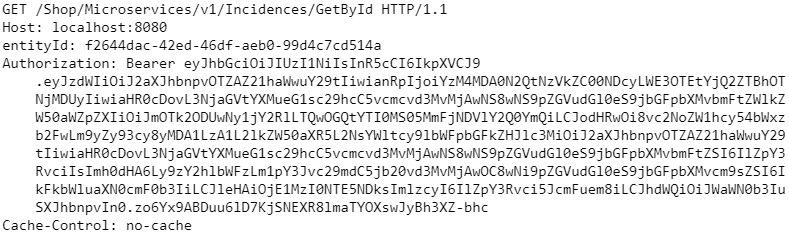
\includegraphics[scale=0.8]{http}
\caption{Ejemplo de petición HTTP donde se incluye un token de seguridad.}
\label{fig:http}
\end{figure}

%%%%%%%%%%%%%%%%%%%%%%%%%%%
% SALTO DE PAGINA
%%%%%%%%%%%%%%%%%%%%%%%%%%%
\newpage

\subsection{Persistencia} \label{subsect:Persistencia}

Para la persistencia se va a emplear \textbf{Entity Framework Core} para el mapeo objeto-relacional y una base de datos SQL en la nube de \textbf{Microsoft Azure}. Entity Framework Core es una versión multiplataforma del ORM Entity Framework (EF) para trabajar con una base de datos mediante objetos .NET. \footnote{Descripción general de Entity Framework Core: \url{https://docs.microsoft.com/es-es/ef/core/}}

Vamos a seguir una aproximación \textit{Code-First} para el diseño de la base de datos. Esta aproximación nos permite diseñar primero las entidades de nuestro dominio a través de las clases en la capa de dominio y luego trasladar sus atributos y relaciones a un esquema de base de datos gracias a EF. \footnote{What is Code-First?: \url{http://www.entityframeworktutorial.net/code-first/what-is-code-first.aspx}}

Para la creación de la base de datos se debe ir al portal de Azure \footnote{ Portal de Azure: \url{https://portal.azure.com/}} y navegar hasta la página SQL Databases. Se debe proveer principalmente su nombre, la suscripción a la que se redirigirán los costes asociados, el grupo de recursos en el que se incluirá y el servidor donde se emplazará. En la figura \ref{fig:CreateDB} se muestra el formulario principal para proveer estos datos.

\begin{figure}[h]
\centering
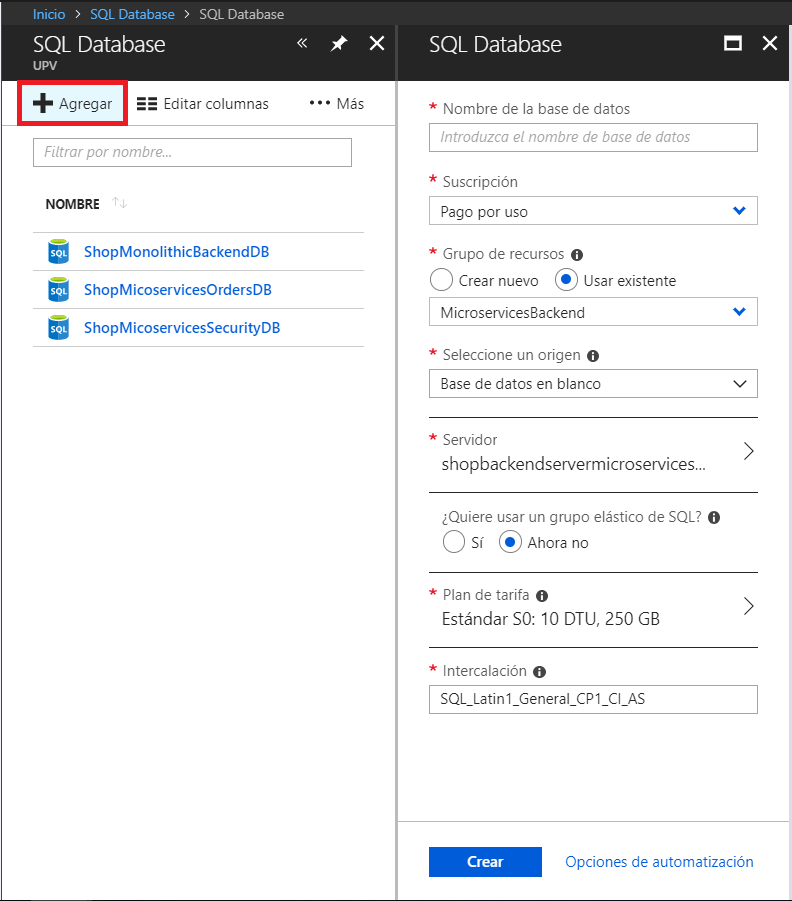
\includegraphics[scale=0.4]{CreateDB}
\caption{Creación de una base de datos SQL en Azure.}
\label{fig:CreateDB}
\end{figure}

Una vez creada, debemos ir al recurso y en la pestaña de cadenas de conexión copiar la asociada a .NET. La cadena de conexión la pegaremos en el archivo de configuración (\textit{appsettings.json}) de la capa de servicios. En la clase \textit{Startup} del mismo proyecto leeremos la cadena de conexión para configurar la clase \textit{ShopContext}, como se observa en la figura \ref{fig:AddDbContext}.

\begin{figure}[h]
\centering
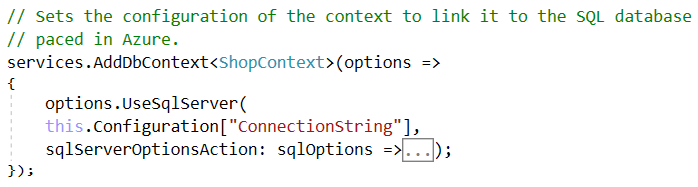
\includegraphics[scale=0.7]{AddDbContext}
\caption{Configuración del contexto de la capa de persistencia para apuntar a la BD en Azure.}
\label{fig:AddDbContext}
\end{figure}

En la clase \textit{ShopContext} debemos indicar cuáles son las entidades del dominio que se añadirán como tablas a la BD. Para cada entidad del dominio se creará un \textit{DbSet} distinto. Se puede ver un fragmento de esta clase en la figura \ref{fig:ShopContext}, que es interna al proyecto para evitar que desde otras capas se realicen operaciones no permitidas.

\begin{figure}[h]
\centering
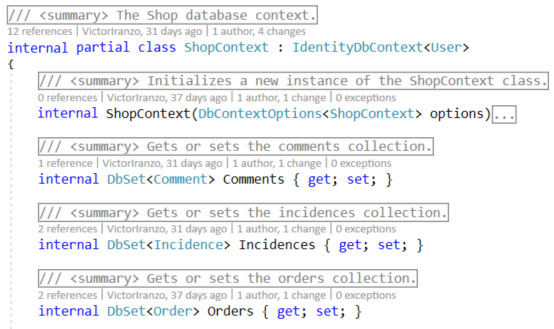
\includegraphics[scale=0.8]{ShopContext}
\caption{Clase ShopContext.}
\label{fig:ShopContext}
\end{figure}

Por último, para que desde otras capas accedan a los datos emplearemos el \textbf{patrón DAO}. Exponer el contexto entero fuera de la capa de persistencia puede ser peligroso porque permitiría modificar desde otras capas aspectos que solo deben conocerse en esta capa. Por ello, se definirá para cada entidad del dominio una interfaz para acceder a sus datos donde las operaciones permitidas están acotadas.

%%%%%%%%%%%%%%%%%%%%%%%%%%%
% SALTO DE PAGINA
%%%%%%%%%%%%%%%%%%%%%%%%%%%
\newpage

\subsection{Informes empleando la librería Open XML PowerTools}

La generación de informes es una de las funcionalidades más empleadas en los software de gestión. En los requisitos de nuestro sistema solo se ha establecido un informe: la factura de un pedido. Esto no implica que debamos dejar de seguir el principio de responsabilidad única. La lógica para generar un informe debe ser genérica para que no dependa del tipo de informe que se va a generar y así pueda ser invocada desde diferentes sitios. Vamos a hacer uso de la librería \textbf{Open XML PowerTools} para la generación de informes.

Open XML PowerTools provee funcionalidades para la combinación de documentos, la conversión de estos a diferentes formatos y la creación de informes a partir de plantillas. \footnote{ Página de GitHub de Open XML PowerTools: \url{https://github.com/OfficeDev/Open-Xml-PowerTools}}. Para generar un informe se separan explícitamente los datos que lo originan y la plantilla del documento. En las plantillas se define cómo se van a renderizar los datos mediante un lenguaje basado en anotaciones. Este lenguaje nos permite escribir contenido en base a condiciones, iterar sobre las colecciones en los datos, crear tablas, etc.

La figura \ref{fig:Factura} muestra la plantilla para generar una factura. La anotación que más se emplea es \textit{Content Select}, que obtiene, a partir de un camino, una cadena de texto (\textit{string}) localizada en los datos provistos. Por ejemplo, el camino \textit{``./Client"} atraviesa los datos ordenados de forma jerárquica hasta alcanzar el nodo etiquetado como Client, donde se almacena el nombre del cliente.

\begin{figure}[h]
\centering
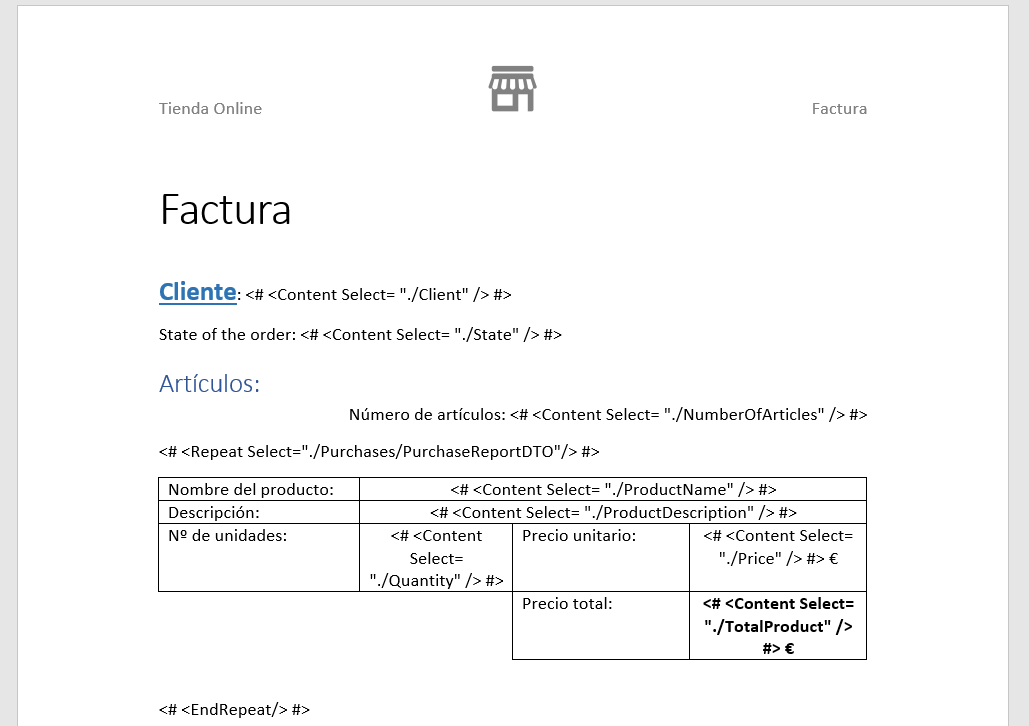
\includegraphics[scale=0.5]{Factura}
\caption{Plantilla para la creación de facturas.}
\label{fig:Factura}
\end{figure}

Las plantillas se almacenarán en la base de datos y cuando se quiera generar un informe se recuperará esta para ensamblar el informe. Los métodos para generar un informe concreto estarán expuestos en los \textit{managers} de la entidad asociada al informe. Por ejemplo, el método para generar la factura de un pedido se situará en el \textit{OrdersManager}. En su implementación, se recuperarán los datos para generar la factura y se enviarán estos al \textit{manager} de informes para que los combine con la plantilla de la factura.

%%%%%%%%%%%%%%%%%%%%%%%%%%%
% SALTO DE PAGINA
%%%%%%%%%%%%%%%%%%%%%%%%%%%
\newpage

\subsection{Notificaciones con la librería MailKit}

Con las notificaciones ocurre lo mismo que con los informes: solo existe un caso de uso que envíe una notificación al cliente, pero para segregar responsabilidades vamos a crear un \textit{manager} específico para este propósito. Para enviar notificaciones se va a hacer uso de la librería \textbf{MailKit}, una librería multiplataforma con utilidades sobre los protocolos IMAP, POP3 y SMTP.

Para desacoplar los mensajes a enviar y el código para enviarlo se hará uso de un DTO que contenga el usuario destinatario, el asunto del correo y el cuerpo del mismo. Tanto el cuerpo como el asunto de la notificación se definirán en archivos de recursos en la capa de aplicación.

\subsection{Inyección de dependencias}

La \textbf{inyección de dependencias} (DI) es un mecanismo para desacoplar un objeto de sus colaboradores. En lugar de instanciar o obtener una referencia a los objetos de los que depende una clase, estos se declaran en el constructor de la clase y es el sistema quien automáticamente los resuelve e instancia. \footnote{ Inserción de dependencias en ASP.NET Core: \url{https://docs.microsoft.com/es-es/aspnet/core/fundamentals/dependency-injection}} En la figura \ref{fig:ProductsManager} se puede ver como se inyecta en el constructor del \textit{manager} de productos el conversor de entidad a DTO y el DAO de la entidad.

\begin{figure}[h]
\centering
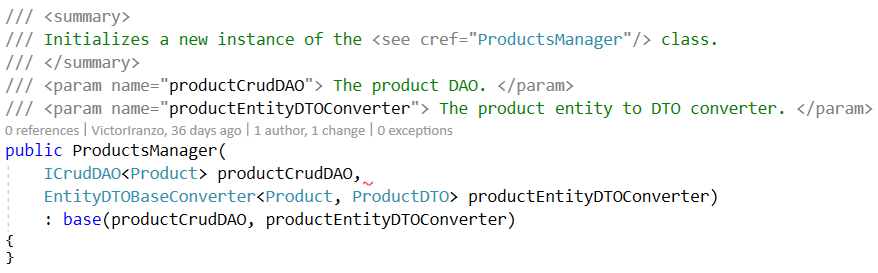
\includegraphics[scale=0.8]{ProductsManager}
\caption{Constructor de la clase ProductsManager donde se aplica DI.}
\label{fig:ProductsManager}
\end{figure}

El uso de interfaces reduce el acoplamiento entre la definición de las operaciones de una clase y las implementaciones concretas que esta definición puede tener. Sin embargo, es necesario indicar con qué implementación se resuelve una interfaz cuando esta se inyecta en el constructor de una clase. Para ellos, se emplean una serie de métodos sobre la colección de servicios donde el sistema busca sus dependencias para indicar cómo resolver cada interfaz. En nuestra solución, cada capa es responsable de registrar las diferentes interfaces que contiene junto con la clase que la implementa. De esta forma, desde otras capas se podrán usar las interfaces resultas.

\subsection{Documentando la API con Swagger UI}

\textbf{Swagger} es un conjunto de herramientas de código abierto para describir la estructura de una API, crear clientes para consumirla en diferentes lenguajes (Swagger CodeGen) y documentarla para que los usuarios puedan emplearla de forma interactiva (Swagger UI). \footnote{ Documentación oficial de Swagger: \url{https://swagger.io/docs/specification/2-0/what-is-swagger/}}

En este apartado nos centraremos en la construcción de la API interactiva. Para hacerlo, basta con añadir la siguiente pieza de código (figura \ref{fig:SwaggerUI}) en la clase \textit{Startup} de la capa de servicios. Aparte de proveer algunos metadatos como la versión de la API o su mantenedor, se debe indicar que los controladores para generar la documentación se encuentran en el ensamblado actual.

\begin{figure}[h]
\centering
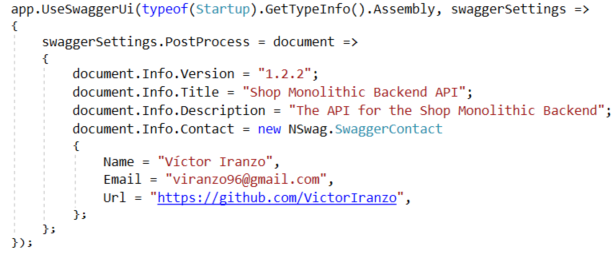
\includegraphics[scale=0.9]{SwaggerUI}
\caption{Metadatos de la API especificados en la clase Startup.}
\label{fig:SwaggerUI}
\end{figure}

La documentación de la API se genera en la dirección formada por la unión de la URL del servidor y el recurso con nombre swagger, como se muestra en la figura \ref{fig:SwaggerAPI}. Para generar la documentación de los métodos, Swagger hace uso de la documentación del método del controlador de la capa de servicios que la origina. En la documentación de cada método se incluye información como la descripción de los parámetros o el tipo de respuesta que da el método.

\begin{figure}[h]
\centering
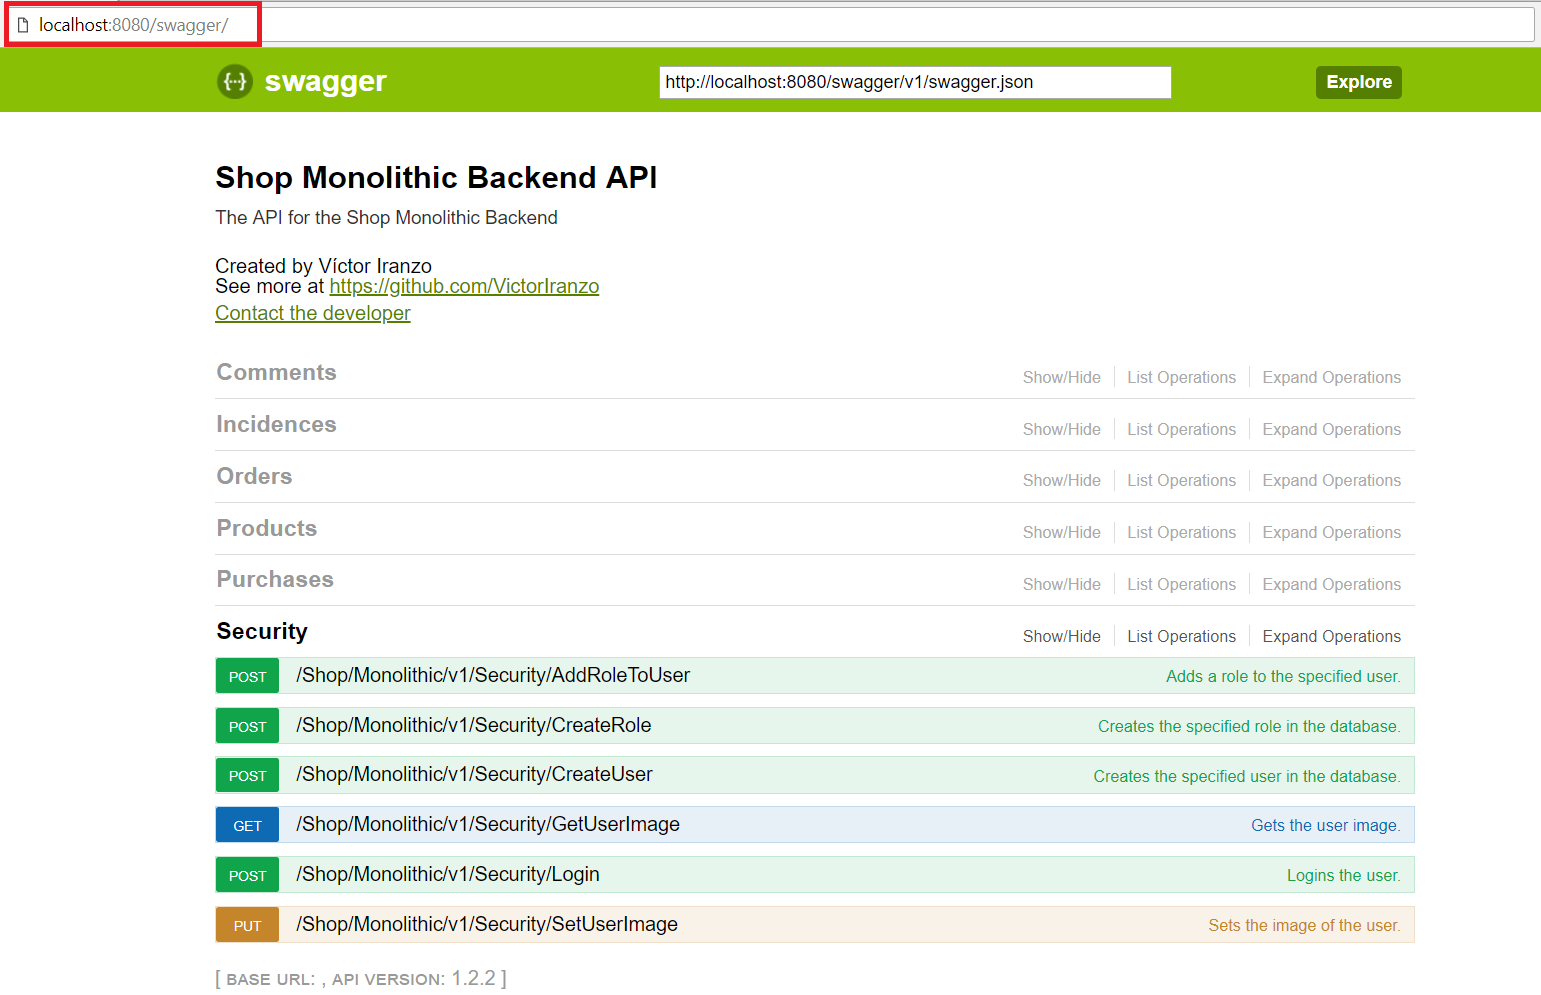
\includegraphics[scale=0.4]{SwaggerAPI}
\caption{Documentación de la API generada con Swagger UI.}
\label{fig:SwaggerAPI}
\end{figure}

\subsection{Generación de la capa de proxy}
%TODO Incluir algo más de NSwag.

Como hemos comentado en la sección \ref{sct:DiseñoMonolitico} \nameref{sct:DiseñoMonolitico}, la capa de proxy se emplea para invocar a la API de la parte servidora a través de llamadas HTTP. Para cada una de las interfaces de contratos vamos a crear un proxy, que implementará sus métodos delegando en un cliente HTTP generado automáticamente con \textbf{NSwag}. NSwag es un conjunto de herramientas para varias plataformas, entre ellas .NET Core, para la generación de especificaciones Swagger a partir de los controladores definidos en C\# y la generación de clientes HTTP para el consumo de estos controladores. \footnote{ Página de GitHub de NSwag: \url{https://github.com/RSuter/NSwag}} \footnote{ NSwag Tutorial: How to integrate NSwag into your ASP.NET Core Web API project: \url{https://www.youtube.com/watch?v=lF9ZZ8p2Ciw}}

El cliente HTTP autogenerado es inyectado en el proxy a través del constructor. El proxy también es el encargado de adaptar los parámetros de la interfaz de contratos a los parámetros que espera el cliente HTTP. Esta adaptación es necesaria porque, por ejemplo, en las peticiones HTTP para los métodos GET no se puede especificar un Body. Como consecuencia, todos los parámetros se deben pasar a través de la cabecera de la petición. De esta forma, los parámetros solo pueden ser de tipos simples como una cadena (\textit{string}) y objetos muy utilizados como los identificadores (\textit{Guid}) han de ser transformados a tipos más simples. 

En la figura \ref{fig:OrdersProxy} se muestra el proxy de pedidos, donde los parámetros de tipo \textit{Guid} son transformados a una cadena de texto mediante la invocación del método \textit{ToString}.

\begin{figure}[h]
\centering
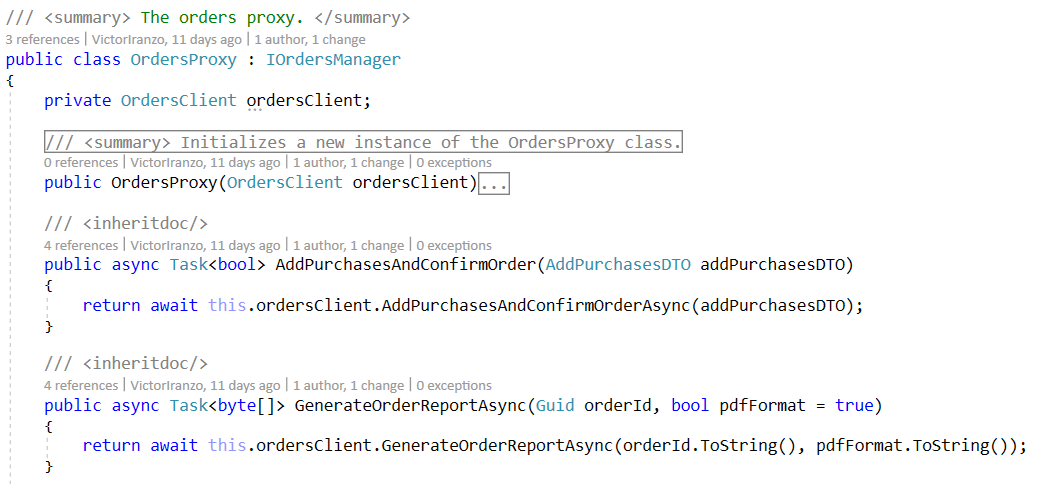
\includegraphics[scale=0.7]{OrdersProxy}
\caption{Fragmento del proxy de pedidos donde se adaptan los parámetros a tipos simples.}
\label{fig:OrdersProxy}
\end{figure}

\subsection{Calidad del código}
%TODO Uso de variables con nombre descriptivo, TODOs

Para asegurar la calidad del código se ha hecho uso de dos herramientas: CodeMaid y StyleCop.

\begin{itemize}

\item \textbf{CodeMaid}: es una extensión de Visual Studio para la limpieza automática de código C\# y otros lenguajes. En el proceso de limpieza, CodeMaid ordena los métodos y propiedades de acuerdo a los estándares, revisa el formato de los comentarios, elimina las referencias a espacios de nombres que no se emplean, etc. \footnote{ Página oficial de CodeMaid: \url{http://www.codemaid.net/}}

\item \textbf{StyleCop}: es un analizador estático de código C\# desarrollado por Microsoft. Se basa en reglas centradas en aspectos como la documentación, la ordenación de los elementos o el estilo de código. Además, permite configurar las reglas que se aplican, definir excepciones a una de ellas o la creación de reglas propias. \footnote{Página de la Wikipedia de StyleCop: \url{https://en.wikipedia.org/wiki/StyleCop}}

\end{itemize}

En la mayoría de proyectos se ha configurado para que las alertas que devuelve StyleCop cuando no se cumple una regla se trate como un error y no como una alerta. Esto se puede conseguir añadiendo la opción TreatWarningsAsErrors en los archivos .csproj.

\section{Interfaz de usuario}

Como hemos comentado en la sección \ref{sct:PlanTrabajo} \nameref{sct:PlanTrabajo}, vamos a implementar una interfaz de usuario que cumpla con los casos de uso y se pueda emplear para comunicar tanto con la solución monolítica como con la basada en microservicios. Para desacoplar el desarrollo del \textit{back-end} y el \textit{front-end}, la aplicación móvil va a desarrollarse en un repositorio de código distinto.

%TODO Decidir si poner esto. https://techcrunch.com/2017/05/11/microsoft-now-lets-ios-developers-deploy-run-and-test-their-apps-directly-from-windows/
Como se observa en la figura \ref{fig:ShopFrontEnd}, la solución de la UI está compuesta por dos proyectos. El primero es en el que se localiza la mayoría del código que se ha implementado, un proyecto .NET Standard con el código compartido por todas las plataformas. El segundo es el proyecto específico para la plataforma Android. Los proyectos asociados a las plataformas UWP y iOS han sido eliminados para hacer más simple su desarrollo.

\begin{figure}[h]
\centering
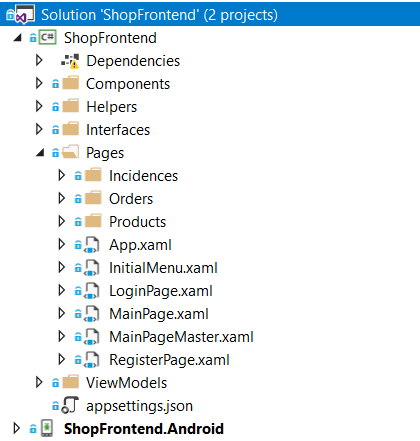
\includegraphics[scale=0.8]{ShopFrontEnd}
\caption{Solución de la interfaz de usuario hecha con Xamarin.Forms.}
\label{fig:ShopFrontEnd}
\end{figure}

Podemos citar las siguientes características que se desean poner en valor de la implementación de la interfaz de usuario:

\begin{itemize}

\item \textbf{Presentación de resultados de forma paginada}: en el \textit{back-end} se han implementado diferentes métodos para obtener resultados (como la lista de incidencias de un usuario o la lista de productos) de forma paginada, ordenada y a través de filtros. La paginación en las invocaciones a una API son una forma de mejorar el rendimiento de una aplicación porque evita traer más resultados de los que luego se consultan. El filtrado y la ordenación de los datos están más centrados en mejor la experiencia del usuario (UX).\footnote{ REST API Design: Filtering, Sorting, and Pagination: \url{https://www.moesif.com/blog/technical/api-design/REST-API-Design-Filtering-Sorting-and-Pagination/}} 

A nivel de UI se ha implementado de tal forma que se soliciten al \textit{back-end} una cantidad de datos aproximada a la que se puede mostrar en la pantalla de un dispositivo. Cuando el usuario haga \textit{scroll} para mostrar más resultados, se realizará una nueva petición en segundo plano a la parte servidora solicitando el siguiente bloque de datos. Mientras se cargan los datos, el usuario visualizará un elemento que indica que el sistema está trabajando en segundo plano para traer más datos.


%TODO Interesante https://msdn.microsoft.com/en-us/magazine/dd419663.aspx https://blogs.msdn.microsoft.com/johngossman/2005/10/08/introduction-to-modelviewviewmodel-pattern-for-building-wpf-apps/
\item \textbf{Uso de \textit{ViewModels}}: la separación de responsabilidades no es un principio que se deba aplicar solo en el back-end. El patrón arquitectónico \textbf{\textit{Model-View-ViewModel}} (MVVM) divide la interfaz de usuario en 3 capas: la vista, empleando páginas XAML, los datos tal como se obtienen en su origen, también llamados el modelo, y el modelo de la vista, que conecta ambos y se utiliza para rellenar la vista. \footnote{From Data Bindings to MVVM: \url{https://docs.microsoft.com/es-es/xamarin/xamarin-forms/xaml/xaml-basics/data-bindings-to-mvvm}}

La diferencia entre este patrón y otros como el \textit{Model-View-Controller} (MVC) es que en MVC los datos con los que se llena la vista son los que se obtienen en el origen y es el controlador quien ha de adaptarlos a cómo se visualizan en la vista. En cambio, en MVVM la vista y el modelo de la vista suelen relacionarse a través de enlaces (\textit{bindings}) en el propio XAML y se notifican mutuamente cuando alguna de sus propiedades cambia. \footnote{ Patterns - WPF Apps With The Model-View-ViewModel Design Pattern: \url{https://msdn.microsoft.com/en-us/magazine/dd419663.aspx}}

Sin embargo, usar este patrón puede ser excesivo para UIs muy sencillas. \footnote{Advantages and disadvantages of M-V-VM: \url{https://blogs.msdn.microsoft.com/johngossman/2006/03/04/advantages-and-disadvantages-of-m-v-vm/}} Por este motivo, hemos usado objetos \textit{ViewModel} en solo aquellos casos que era necesario adaptar los datos del modelo a la vista. Lo que aquí definimos como modelo es un DTO que devuelve la parte servidora y ya está diseñado para que contenga solo la información estrictamente necesaria. Un ejemplo en el que se emplea un \textit{ViewModel} es el \textit{ProductViewModel} (figura \ref{fig:ProductViewModel}), donde se tiene que transformar la imagen que se recibe del ProductDTO de una \textit{byte array} a un \textit{ImageSource}.

\begin{figure}[h]
\centering
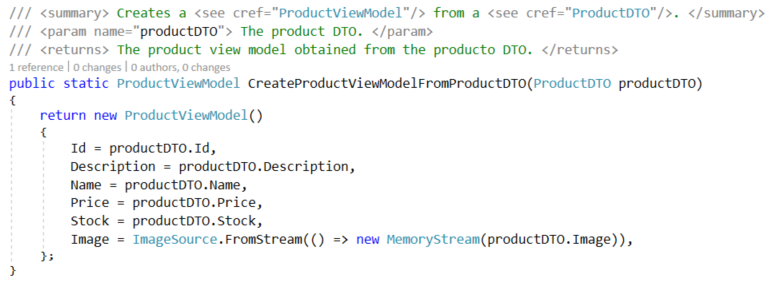
\includegraphics[scale=0.8]{ProductViewModel}
\caption{Método para transformar de un DTO a un modelo de una vista.}
\label{fig:ProductViewModel}
\end{figure}

\item \textbf{Código específico de plataforma}: existen algunos servicios que no se pueden implementar en el proyecto compartido por todas las plataformas. Estos servicios están relacionados con aspectos muy ligados a cada plataforma, como puede ser el sistema de archivos. Para este propósito se define una interfaz en el proyecto compartido. Cada una de las plataformas debe dar una implementación concreta a esta interfaz. Desde el proyecto genérico, se hace uso de la interfaz y será el sistema quien se encargará de dirigir la operación que se invoca sobre la interfaz a la implementación de la plataforma. \footnote{Native Services with Xamarin.Forms? It's DependencyService to the Rescue: \url{https://visualstudiomagazine.com/articles/2015/09/01/native-services-with-xamarinforms.aspx}}

\end{itemize}

Como material adicional, en el apéndice \ref{ch:ModeloNavegacion} \nameref{ch:ModeloNavegacion} se incluyen capturas de la aplicación desarrollada y la navegación que existe entre las diferentes pantallas.

\section{Pruebas} \label{sect:MonoPruebas}

Se han realizado un total de 16 pruebas automatizadas mediante el framework \textbf{NUnit}. NUnit es una librería para la implementación de pruebas unitarias en todos los lenguajes .NET al igual que JUnit lo es para el lenguaje Java. \footnote{ Página de GitHub de NUnit: \url{https://github.com/nunit/nunit}}. La mayoría de las pruebas realizadas se clasifican como pruebas de integración porque involucran a más de una clase. 

No se han podido probar todos los métodos expuestos en la interfaz del \textit{back-end}, pero gracias a que existe mucho código genérico para la realización de operaciones CRUD y la persistencia de datos, podemos considerar el sistema como fiable. Algunas de las pruebas que si se han hecho son las asociadas a los casos de uso CU003, CU004, CU005, CU007, CU009 y CU013 que se encuentran en la sección \ref{sect:CUs} \nameref{sect:CUs}. El resumen de las pruebas realizadas y su correcta ejecución se muestran en la siguiente figura.

\begin{figure}[h]
\centering
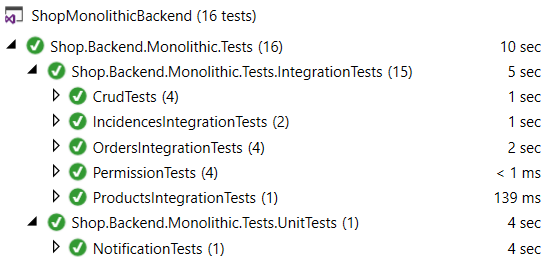
\includegraphics[scale=0.8]{Tests}
\caption{Pruebas realizadas en la solución monolítica.}
\end{figure}

Para la realización de las pruebas se ha empleado una base de datos en memoria. Así, las pruebas son más cercanas a una situación real. A la vez, no añade un sobrecoste asociado al acceso a datos de una base de datos real, que haría más lenta la ejecución de las pruebas. \footnote{ Pruebas con InMemory: \url{https://docs.microsoft.com/es-es/ef/core/miscellaneous/testing/in-memory}} Además, en el método \textit{Setup} que se invoca antes de cada prueba es donde se resuelven las dependencias declaradas en los constructores de las clases invocando a los métodos \textit{AddDependencies} de las capas de aplicación y persistencia, como muestra la figura \ref{fig:SetupTest}. 

\begin{figure}[h]
\centering
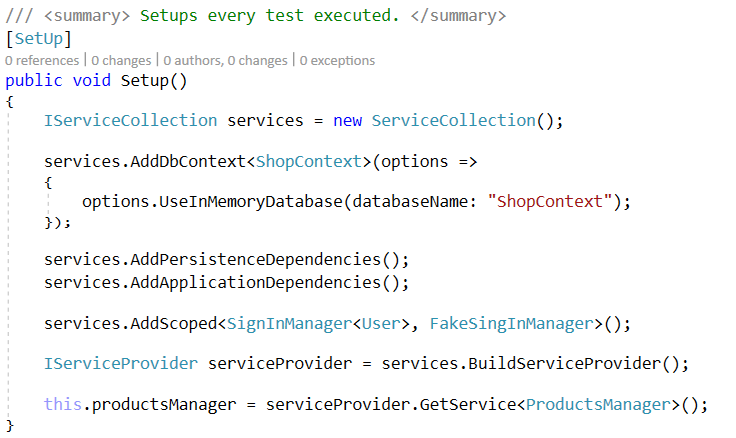
\includegraphics[scale=0.8]{SetupTest}
\caption{Ejemplo de método Setup donde se emplea una base de datos en memoria.}
\label{fig:SetupTest}
\end{figure}

Por último, para algunos servicios provistos por las herramientas utilizadas se han tenido que implementar \textit{fakes}. Es el caso del manager de Identity para hacer login en la aplicación, que se debe sobreescribir para devolver que el usuario ha hecho login correctamente sin acceder a la base de datos de usuarios.

%%%%%%%%%%%%%%%%%%%%%%%%%%%
% SALTO DE PAGINA
%%%%%%%%%%%%%%%%%%%%%%%%%%%
\newpage

\section{Despliegue de la solución monolítica}

Como hemos mencionado en la sección \ref{sect:Propuesta} \nameref{sect:Propuesta}, para el despliegue de la aplicación se va a hacer uso de Azure App Service. No se va a implementar ninguna \textit{pipeline} para desplegar automáticamente y todos los pasos que se detallan se deben hacer manualmente, aunque sean muy sencillos:

\begin{enumerate}

\item \textbf{Creación de un Dockerfile}: en la capa de servicios se debe crear un Dockerfile. En la mayoría de ejemplos encontrados se ha visto que la imagen de Docker se genera básicamente mediante dos pasos del Dockerfile: se copian todos los archivos de la solución a la imagen y se compila la solución completo. Cuando se crea y arranca un contenedor, se inicia el proceso del servicio a través de la DLL que se ha generado tras la compilación. \footnote{ Dockerize a .NET Core application
: \url{https://docs.docker.com/engine/examples/dotnetcore/\#create-a-dockerfile-for-an-aspnet-core-application}} Este Dockerfile es más fiable en cuanto a que los ensamblados necesarios se generan dentro de la propia imagen. Sin embargo, la creación de la imagen es más lenta. Por ello, para entornos de desarrollo vamos a simplificar el Dockerfile para que simplemente copie los ensamblados en la imagen, que se han generado previamente en el entorno de desarrollo. La figura \ref{fig:Dockerfile} muestra su contenido. Los ensamblados se publican dentro de una carpeta que hemos llamado PublishOutput. En el Dockerfile tampoco hace falta exponer ningún puerto porque esto ya lo hace la imagen base.

\begin{figure}[h]
\centering
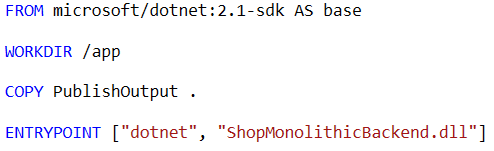
\includegraphics[scale=0.8]{Dockerfile}
\caption{Dockerfile de la solución monolítica.}
\label{fig:Dockerfile}
\end{figure}

\item \textbf{Crear un App Service}: en el portal de Azure, seleccionar la pestaña de nuevo recurso y marcar Web App. Se debe proveer el nombre de la aplicación, que será la URL donde luego encontraremos nuestro servicio, la suscripción y el grupo de recursos. También se debe crear un plan de App Service, donde se establecerán las prestaciones del servidor donde se desplegará y las tarifas asociadas. 

\item \textbf{Obtener perfil de publicación}: una vez creado el recurso nos podemos descargar el perfil de publicación desde el panel del recurso. Desde aquí también  podemos iniciar y detener el servicio (figura \ref{fig:AppService2}).

\begin{figure}[h]
\centering
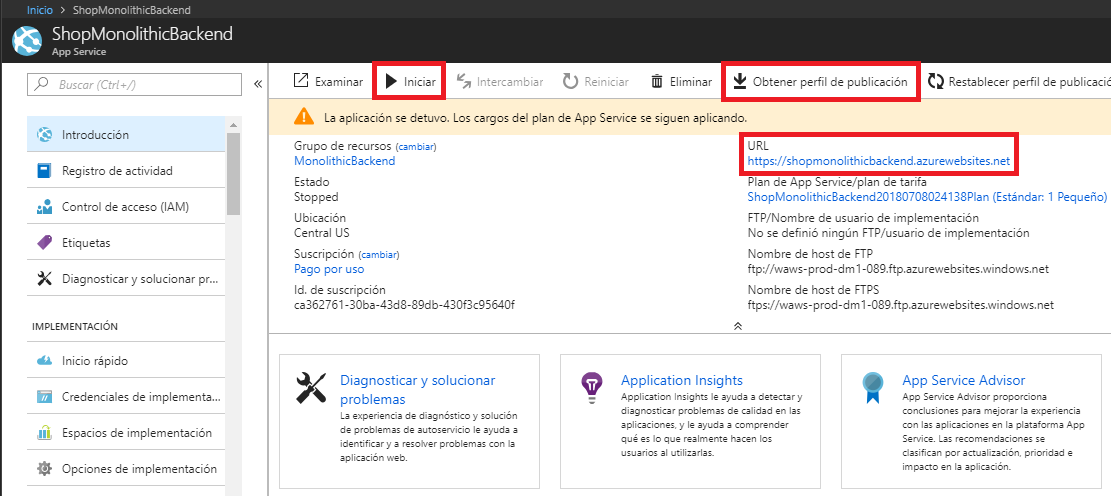
\includegraphics[scale=0.6]{AppService2}
\caption{Recurso App Service en el portal de Azure.}
\label{fig:AppService2}
\end{figure}

\item \textbf{Importar perfil de publicación}: desde la solución de Visual Studio, abrir el menú contextual del proyecto de la capa de servicios y seleccionar la opción ``Publish". En la ventana que se abre seleccionar ``New profile" y luego ``Import profile", donde seleccionaremos el archivo que nos hemos descargado.

\item \textbf{Desplegar el servicio}: cada vez que queramos desplegar a producción una nueva versión de la API nos iremos al proyecto de servicios en Visual Studio, abriremos el menú de publicación a través del menú contextual y seleccionaremos el perfil de AppService. Las opciones principales que desde este formulario se pueden realizar se han resaltado en la figura \ref{fig:AppService3}. Si accedemos a la URL que antes hemos señalado, veremos la documentación de la API generada por Swagger UI.

\begin{figure}[h]
\centering
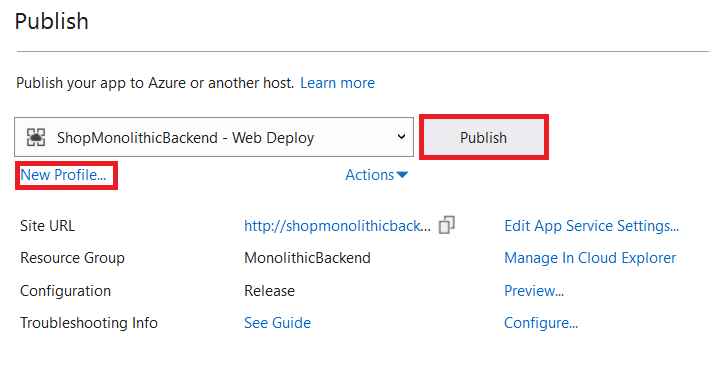
\includegraphics[scale=0.6]{AppService3}
\caption{Despliegue a través de App Service.}
\label{fig:AppService3}
\end{figure}

\end{enumerate}

%%%%%%%%%%%%%%%%%%%%%%%%%%%%%%%%%%%%%%%%%%%%%%%%%%%%%%%%%%%%%%%%%%%%%%%%%%%%%%%
%                       MICROSERVICIOS
%
%%%%%%%%%%%%%%%%%%%%%%%%%%%%%%%%%%%%%%%%%%%%%%%%%%%%%%%%%%%%%%%%%%%%%%%%%%%%%%%

\chapter{Diseño e implementación de la solución basada en microservicios}

A lo largo del capítulo anterior nos hemos centrado sobre todo en aspectos de implementación relacionados con diferentes herramientas como Identity o Swagger. En este capítulo nos vamos a centrar más en el diseño ya que, como hemos dicho en el apartado \ref{sct:PlanTrabajo} \nameref{sct:PlanTrabajo}, vamos a refactorizar la solución monolítica y a nivel de código apenas va a verse modificada.

\section{Diseño de la solución}

Para la descomposición de la solución en microservicios vamos a aplicar los principios que hemos explicado en el apartado \ref{sct:FaseDiseño} \nameref{sct:FaseDiseño}. Se tienen que extraer contextos bien delimitados sin importar en un primer momento el tamaño de estos. Aunque contemos con la experiencia del desarrollo de la solución monolítica, el tamaño de los microservicios se puede ajustar más adelante evaluando si vale la pena dividir un microservicio.

Concretamente, para representar visualmente la división en contextos delimitados se va emplear el modelo de dominio del caso de estudio, como se muestra en la figura \ref{fig:ShopBoundedContexts}. A continuación, detallamos cada uno de ellos, centrándonos en las capacidades que ofrece al negocio y no tanto en las entidades que maneja:

\begin{figure}[h]
\centering
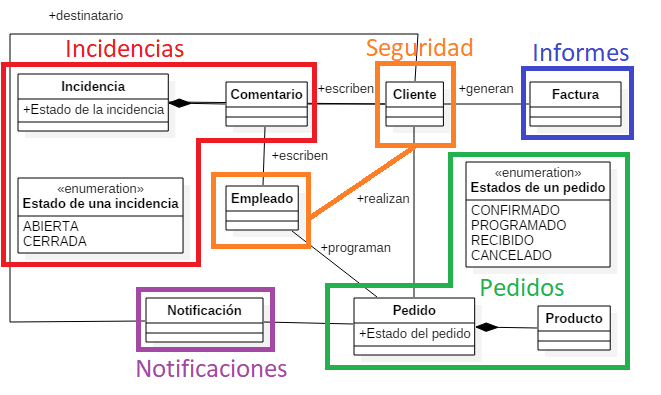
\includegraphics[scale=1]{ShopBoundedContexts}
\caption{División del modelo de dominio en contextos delimitados.}
\label{fig:ShopBoundedContexts}
\end{figure}

\begin{itemize}

\item \textbf{Incidencias}: permite la creación de incidencias, obtener las incidencias de un cliente y añadir comentarios dentro de una incidencia.

\item \textbf{Seguridad}: ofrece las funcionalidades de registro de nuevos clientes y \textit{login}. Además, persiste los datos de los clientes, por lo que algunos de los microservicios tendrán una referencia a este, por ejemplo, para obtener el cliente o empleado que escribió un comentario.

\item \textbf{Informes}: es un motor que almacena las plantillas de los informes que se pueden generar y combina estas con los datos que recibe para generar un documento de salida. No ofrece directamente ninguna funcionalidad al cliente: se trata de un \textbf{microservicio interno} que otros servicios emplean.

\item \textbf{Notificaciones}: al igual que el microservicio de informes, no está ligado a ningún tipo de dato. Simplemente, ofrece la funcionalidad de enviar una notificación con el contenido que recibe como parámetro al destinatario especificado. También es un microservicio interno.

\item \textbf{Pedidos}: permite obtener los pedidos de un cliente, generar la factura de un pedido, añadir productos...En este servicio se ha incluido la entidad Producto. Podríamos diseñar un microservicio de catálogo aparte. A este servicio solo tendrían acceso los empleados del comercio para gestionar el número de unidades en stock o la creación de nuevos productos. Sin embargo, ninguna funcionalidad fuera del contexto de los pedidos se relaciona con los productos, por lo que en este servicio la entidad producto y más adelante evaluaremos si vale la pena representarla dentro de un microservicio independiente. 

\end{itemize}

\subsection{Arquitectura interna de los microservicios}

En el apartado \ref{subsec:Poliglota} \nameref{subsec:Poliglota} se ha reflexionado sobre que una arquitectura basada en microservicios permite emplear diferentes tecnologías, arquitecturas y bases de datos en cada microservicio. Para validar lo que en este apartado se dice, vamos a desarrollar algunos microservicios con diferentes combinaciones de estas 3 características. Las arquitecturas de cada uno de los servicios así como las relaciones de dependencias que existen entre ellos se pueden ver en el diagrama de la figura \ref{fig:Componentes}.

\begin{figure}[h]
\centering
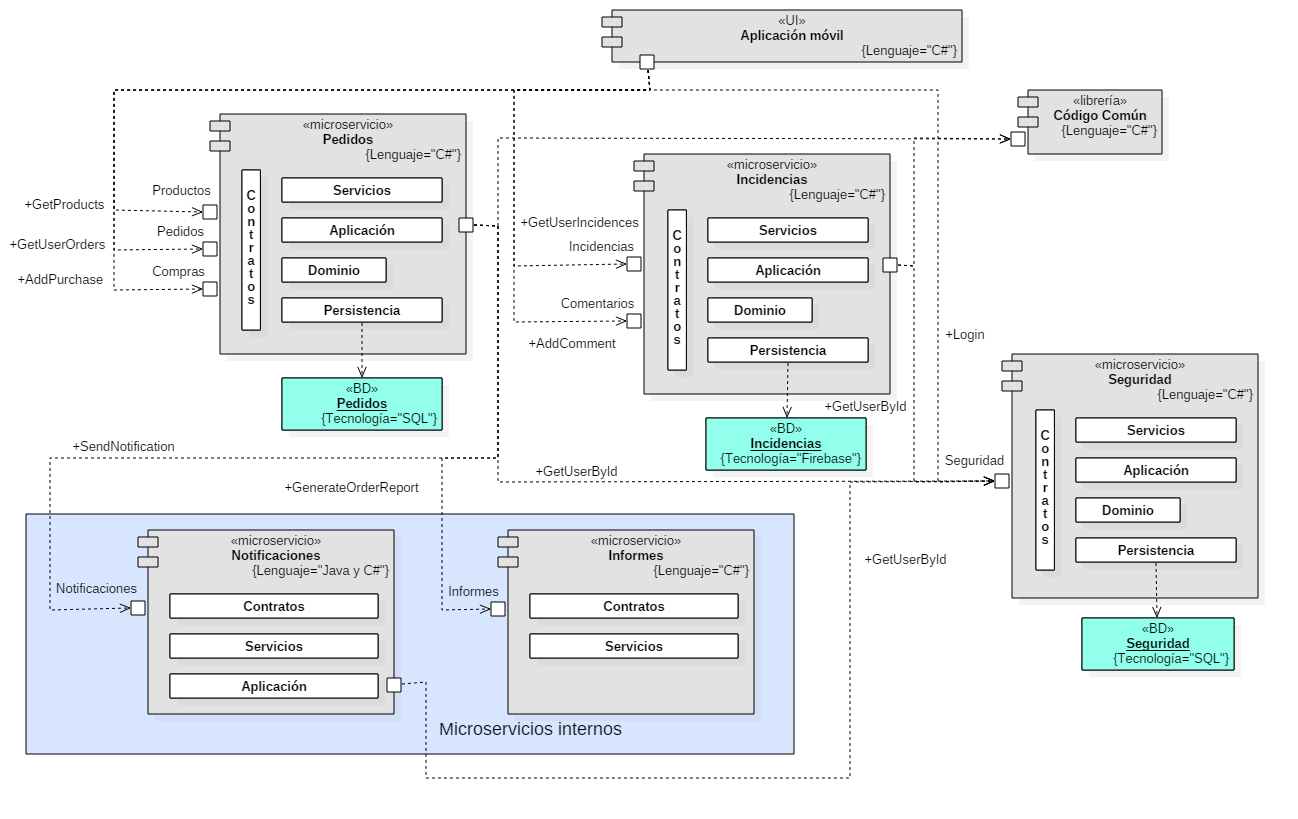
\includegraphics[scale=0.35]{Componentes}
\caption{Diagrama de componentes de la solución basada en microservicios.}
\label{fig:Componentes}
\end{figure}

En la mayoría de microservicios vamos a seguir la arquitectura de 6 capas que se describe en la sección \ref{sct:DiseñoMonolitico} \nameref{sct:DiseñoMonolitico}. Esto hará que su refactorización sea más sencilla ya que solo debemos copiar las clases relacionadas al microservicio en cada una de las capas. 

Cada microservicio tendrá su propia base de datos, aunque estas pueden localizarse dentro del mismo servidor. Para evaluar otra tecnología de base de datos, la BD del servicio de incidencias la vamos a implementar con \textbf{Firebase}.

Las necesidades de cada microservicio de nuestro caso de estudio son diferentes: algunos como el de informes o notificaciones no requieren persistir datos, por lo que aplicar una arquitectura de 6 capas en ellos no es necesario. 

En el microservicio de informes vamos a seguir una arquitectura más sencilla. Su lógica se situará directamente en la capa de servicios, eliminando la capa de aplicación. Las capas de dominio y persistencia también pueden ser eliminadas porque las plantillas de los informes se van a almacenar ahora como un recurso y no en una base de datos. 

En cuanto al servicio de notificaciones, vamos a implementarlo en el lenguaje \textbf{Java}. Sin embargo, como debe ser consumido por microservicios en lenguaje C\#, construiremos un proxy en este lenguaje para hacer más fácil su consumo.

En el capítulo anterior, en las secciones \ref{subsect:CRUD} \nameref{subsect:CRUD} y \ref{subsect:Persistencia} \nameref{subsect:Persistencia} hemos nombrado algunas interfaces e implementaciones genéricas relacionadas con las entidades de dominio. Los microservicios de pedidos e incidencias deben seguir haciendo uso de estas implementaciones. Hacer de este código común un servicio no tiene sentido porque está relacionado con el acceso a datos y cada microservicio es dueño de sus propios datos. En este caso, este código genérico se referencia como una \textbf{librería} a través de paquetes NuGet, que en el diagrama de componentes se muestra con la etiqueta ``Código común".

Por último, indicar que el consumo de cualquier microservicio, ya sea desde la interfaz de usuario o desde otros servicios, se realizará a través de las capas de proxy. En el diagrama de componentes no se ha incluido esta capa en la arquitectura interna de ninguno de los microservicios porque esta capa no se ejecuta en el proceso del servicio.

\subsection{Organización de los microservicios}
%Cesar de la Torre.

En cuanto a la organización de los microservicios, vamos a emplear un único repositorio de código que contenga el código de todos los microservicios. Como en la solución monolítica, cada capa se representará a través de un proyecto .NET y cada microservicio tendrá una solución de Visual Studio distinta.

Newman \cite{Newman2015a} reflexiona sobre esto en relación a las compilaciones de integración continua. Según él, la mejor opción es tener un repositorio y una compilación diferente para cada microservicio. De esta forma, existe una mayor correspondencia entre los servicios y los equipos encargados de cada uno porque cada equipo realiza cambios en un único repositorio. Además, se evita que un simple cambio en un microservicio lance la compilación de toda la solución \cite{Newman2015a}. En nuestro caso, no vamos a aplicar las prácticas de integración continua y tampoco tenemos equipos de trabajo distintos, por lo que será más cómodo utilizar un único repositorio. Como consecuencia, esto implica que en un mismo \textit{commit} se puedan incluir cambios de diferentes microservicios.

En cuanto a la organización en soluciones en Visual Studio, en \cite{DelaTorre2018} se organiza el código de la aplicación desarrollada en un único repositorio con una única solución. Creemos que esta aproximación no es la mejor. No tiene sentido que un desarrollador que trabaja en un único repositorio vea en su solución otros microservicios distintos al suyo. Además, incluir tantos archivos en la solución aumenta su tiempo de compilación, cuando jamás se van a realizar cambios o ejecutar algunos de ellos. Por ello, hemos optado por una solución diferente para cada servicio, como se muestra en la figura \ref{fig:MicroservicesSolution}.

\begin{figure}[h]
\centering
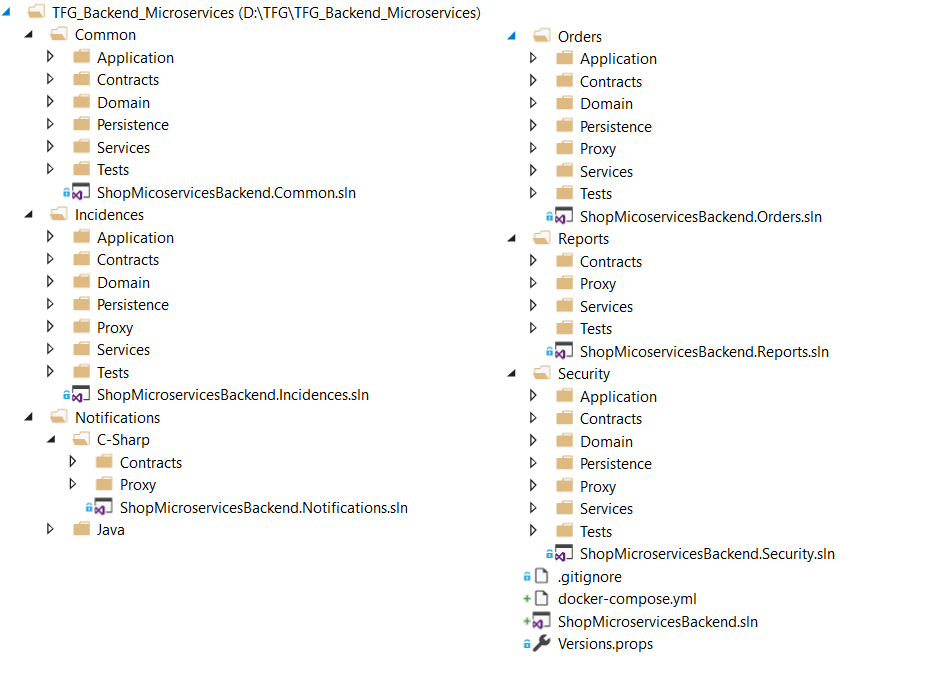
\includegraphics[scale=0.85]{MicroservicesSolution}
\caption{Organización de la solución basada en microservicios.}
\label{fig:MicroservicesSolution}
\end{figure}

%%%%%%%%%%%%%%%%%%%%%%%%%%%
% SALTO DE PAGINA
%%%%%%%%%%%%%%%%%%%%%%%%%%%
\newpage

\section{Diferencias en la implementación respecto a la solución monolítica}

\subsection{Consumo de otros microservicios} \label{subsect:Consumo}

Para que un microservicio pueda hacer peticiones a otro, se deben seguir los siguientes pasos:

\begin{enumerate}

\item Instalar el paquete NuGet del microservicio a consumir en la capa de aplicación (figura \ref{fig:OrdersApplicationDependencies}).

\begin{figure}[h]
\centering
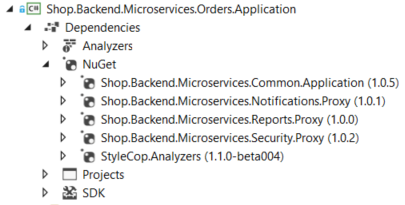
\includegraphics[scale=0.85]{OrdersApplicationDependencies}
\caption{Dependencias del microservicio de pedidos en la capa de aplicación.}
\label{fig:OrdersApplicationDependencies}
\end{figure}

\item Al registrar las dependencias de la capa de aplicación, invocar al código de la capa de proxy donde se registran las interfaces del microservicio a consumir (figura \ref{fig:UsingMicroservices}). Esto significa que en un microservicio cuando hagamos una petición a otro servicio a través de la interfaz se realizará una llamada HTTP a través de su proxy.

\begin{figure}[h]
\centering
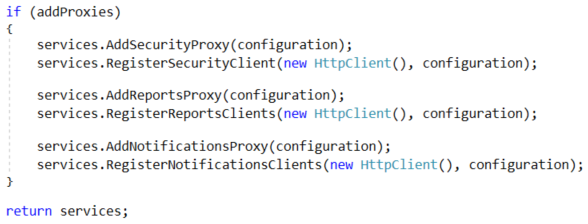
\includegraphics[scale=0.85]{UsingMicroservices}
\caption{Código para resolver otros microservicios consumidos.}
\label{fig:UsingMicroservices}
\end{figure}

\item En el microservicio, inyectar en el constructor la interfaz de contratos del servicio que se desea consumir.

\end{enumerate}

\subsection{Consistencia eventual}
%TODO Escribir cambios en la capa de dominio

Cada servicio es soberano de sus datos y la mejor manera de conseguir esto es separar los datos de cada uno en diferentes bases de datos. Una única base de datos relacional para toda la aplicación, tal y como se usa en la solución monolítica, tiene dos ventajas principalmente: se pueden emplear transacciones atómicas y restricciones de integridad referencial. 

No se puede realizar una transacción única que involucre a diferentes microservicios, sobre todo porque cada uno puede utilizar una tecnología de BD diferente. Las transacciones se deben implementar en la capa de aplicación y en caso de que una operación falle, se deben establecer mecanismos de compensación que reviertan los cambios hechos hasta ese punto \cite{DelaTorre2018}.

Por suerte, las únicas referencias en los datos que hay entre diferentes servicios son las que hay desde incidencias y pedidos al servicio de seguridad. Tanto los pedidos, las incidencias y los comentarios están asociados a un cliente. En caso de que se borre un cliente, se deben borrar en cascada las instancias de estas entidades que tenga asociadas, como si de una transacción se tratara. La operación de eliminar un cliente no está soportada por la API, por lo que no ha sido necesario implementar ninguna transacción entre microservicios.

En caso de que estuviera soportada, no se puede realizar de forma atómica y la consistencia sería eventual. Un usuario podría ver un estado inconsistente del sistema si se ha eliminado un cliente en el microservicio de seguridad pero sus pedidos todavía no. Se denomina eventual porque en algún punto próximo del tiempo la transacción que se ha iniciado entre diferentes microservicios para eliminar a un usuario se completará en todo el sistema.

En cuanto a las restricciones de integridad referencial, en una base de datos relacional se modela a través de claves externas (\textit{foreign key}, FK). Dentro de la base de datos de un servicio podemos emplear FKs, como ocurre en las relaciones entre pedido y compra. Sin embargo, en las relaciones que hemos comentado con el módulo de seguridad, no se pueden usar como tal FKs porque se referenciaría a otra base de datos. En su lugar, se almacena únicamente el identificador de la entidad referenciada y cuando se quiere acceder a ella se debe hacer una petición al servicio que la gestiona. Esto se refleja en las entidades de la capa de dominio, como se ve en la figura \ref{fig:Comment}.

\begin{figure}[h]
\centering
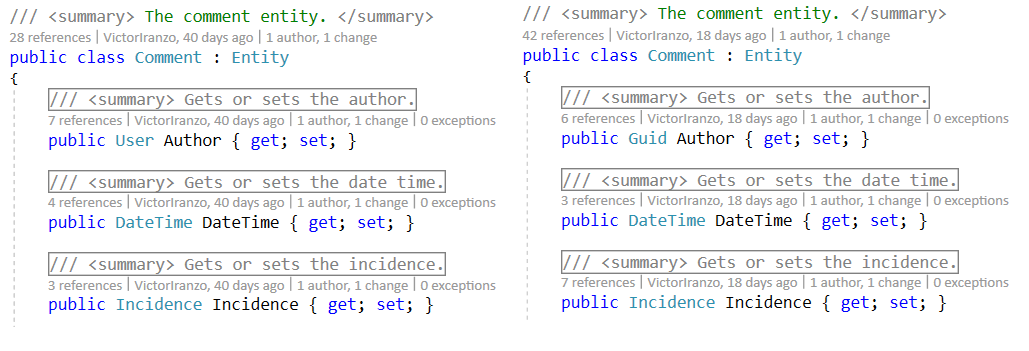
\includegraphics[scale=0.7]{Comment}
\caption{Clases de dominio de la entidad comentario en la solución monolítica (izquierda) y la basada en microservicios (derecha).}
\label{fig:Comment}
\end{figure}

\subsection{Microservicio de notificaciones}

El microservicio de notificaciones ahora está desarrollado en dos lenguajes de programación distintos: Java y C\#.

En C\# está desarrollado todo lo necesario para el consumo del servicio. Esto incluye la capa de contratos (donde se define su interfaz y el DTO que se empleará en la parte C\#) y la de proxy (donde se encuentra el cliente HTTP para realizar peticiones al microservicio). El proyecto C\# del microservicio de notificaciones se muestra en la figura \ref{fig:NotificationsC}.

\begin{figure}[h]
\centering
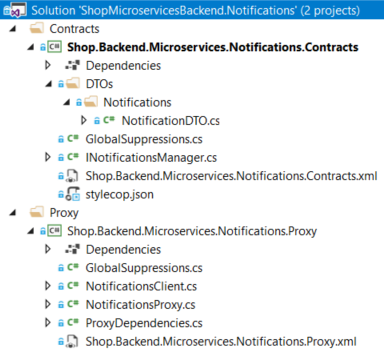
\includegraphics[scale=0.85]{NotificationsC}
\caption{Parte del microservicio de notificaciones desarrollada en C\#.}
\label{fig:NotificationsC}
\end{figure}

En Java se han desarrollado la capa de aplicación y servicios. La implementación de la capa de aplicación para mandar un correo electrónico es trivial. Para la capa de servicios, se crea e inicia un objeto HttpServer al que se le asigna un handler.

El handler es similar a lo que en .NET llamábamos controlador. En nuestro caso, deserializará el cuerpo (\textit{body}) de la petición en un objeto empleando la librería Gson y delegará en la capa de aplicación la operación a realizar. Cuando se quiere consumir otro microservicio no podemos utilizar los proxies que hemos creado para C\# porque es otro lenguaje de programación. En nuestro ejemplo, queremos contactar con el servicio de seguridad para obtener el correo electrónico de un usuario.

Por último, el archivo Dockerfile (figura \ref{fig:JavaDockerfile}) para el despliegue del servicio también varía. Vamos a seguir el mismo criterio que en los contenedores de microservicios .NET de usar los ensamblados (en este caso, un archivo *.jar) para generar la imagen con el menor número de recursos posibles. Tanto el comando para iniciar el proceso del contenedor como la imagen base se verán modificados.

\begin{figure}[h]
\centering
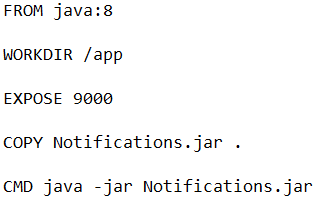
\includegraphics[scale=1]{JavaDockerfile}
\caption{Dockerfile del microservicio de notificaciones.}
\label{fig:JavaDockerfile}
\end{figure}

\subsection{Persistencia en microservicio de incidencias}

En el microservicio de incidencias vamos a emplear una base de datos en la plataforma Firebase. \textbf{Firebase} es una plataforma para el desarrollo de aplicaciones. Uno de los servicios que ofrece es una base de datos NoSQL en la nube en tiempo real. Los datos se almacenan en formato JSON y su acceso puede realizarse a través de peticiones HTTP. \footnote{ Documentación de Firebase Realtime Database: \url{https://firebase.google.com/docs/database/}} 

Una de las principales ventajas de las bases de datos NoSQL es su escalabilidad horizontal. En lugar de tener un gran servidor para alojar una base de datos relacional, una base de datos NoSQL se puede distribuir entre diferentes máquinas. Esta funcionalidad en Firebase es de pago y no vamos a hacer uso de ella. Nuestro objetivo  es validar que diferentes microservicios pueden utilizar tecnologías de bases de datos distintas. En la figura \ref{fig:Firebase} se muestra la estructura jerárquica de la BD de incidencias.

\begin{figure}[h]
\centering
\includegraphics[scale=0.85]{Firebase}
\caption{Base de datos de incidencias en Firebase.}
\label{fig:Firebase}
\end{figure}

Gracias a la arquitectura interna basada en capas, el uso de esta BD solo implica dejar de usar la implementación que se da por defecto al DAO en la librería común y programar una implementación propia que acceda a los datos de Firebase a través de llamadas HTTP.

\section{Versionado de servicios}
% https://www.thomaslevesque.com/2017/09/18/common-msbuild-properties-and-items-with-directory-build-props/

Cada uno de los microservicios se va a desplegar de forma independiente. El consumo de un microservicio se realiza a través de su proxy, que es una implementación de una interfaz de la capa de contratos. Cuando se realiza y se despliega un cambio en un servicio pueden ocurrir dos situaciones respecto a sus consumidores:

\begin{itemize}

\item  La primera situación es que el cambio \textbf{no haya supuesto un cambio en la interfaz} de la capa de contratos. En este caso, se habrá realizado un cambio a nivel de la lógica del servicio o su persistencia, como puede ser la corrección de un defecto. El cambio realizado no necesita ser conocido por sus consumidores porque están desacoplados de la implementación específica del servicio. 

Los consumidores pueden seguir consumiendo la misma versión del servicio. Solo en caso de que se haya modificado el comportamiento del servicio (su especificación) los consumidores deberán ser notificados para adaptarse a cambios en las respuestas del servidor. Por ejemplo, se puede haber cambiado la política de permisos de un método sin haber cambiado su interfaz y ahora devuelve un error 401:Unauthorized porque es necesario otro rol para invocarlo.

\item Una segunda situación consiste en que el cambio \textbf{haya significado un cambio en la interfaz} de contratos. Por ejemplo, puede ocurrir que se haya añadido un nuevo parámetro a un método o se haya cambiado el DTO de respuesta de un método. En este caso, los consumidores deben actualizar el proxy que emplean para comunicar con la nueva versión del servicio. Para asegurar que ningún consumidor se rompe por la actualización se pueden seguir dos aproximaciones, según la literatura:

%TODO Esto está muy relacionado con los despliegues V-A y canary releases.
\begin{itemize}

\item \textbf{Mantener la vieja interfaz y redireccionar internamente las peticiones que recibe a la nueva interfaz.} Ambas interfaces están disponibles hasta asegurarse de que ningún cliente esta empleando la interfaz vieja, lo que requiere de la monitorización del servicio para saber cuántos clientes la consultan todavía.

\item \textbf{Tener diferentes versiones del servicio en funcionamiento.} Las peticiones realizadas a la interfaz antigua se redireccionan a la versión vieja del servicio y al contrario con las nuevas peticiones.

Sin embargo, esta aproximación cuenta con algunas desventajas. En primer lugar, si se debe hacer una modificación como solucionar un defecto, posiblemente se deba hacer y desplegar en ambas versiones del servicio. En segundo lugar, se necesita un middleware con la lógica para redireccionar las peticiones a una u otra versión. En conclusión, esta solución puede resultar apta para periodos cortos de tiempo, pero cuanto más tiempo permanezcan los clientes utilizando la vieja versión del servicio más riesgo tendremos de que ocurran estos problemas \cite{Newman2015a}.

\end{itemize}

\end{itemize}

En nuestro caso de estudio, tenemos control de todos los consumidores ya que la interfaz de los servicios no va a ser publicada para su consumo por aplicaciones de terceros. Los consumidores de un microservicio serán o la interfaz de usuario u otros servicios. Como hemos comentado en la sección \ref{subsect:Consumo} \nameref{subsect:Consumo}, el proxy se añade como un paquete NuGet con una versión específica. Para asegurarnos de que siempre se consume la última versión de un servicio, vamos a hacer uso de variables para referir a la versión del paquete NuGet a instalar, como se puede ver en la figura \ref{fig:Csproj}.

\begin{figure}[h]
\centering
\includegraphics[scale=0.9]{OrdersNuGets}
\caption{Fragmento del proyecto (.csproj) del servicio de pedidos.}
\label{fig:Csproj}
\end{figure}

A estas variables se les da valor en un archivo llamado \textit{Versions.props}. Este archivo está centralizado y es común para todos los servicios para que todos ellos referencien a la misma versión de otro microservicio. \footnote{ Common MSBuild properties and items with Directory.Build.props: \url{https://www.thomaslevesque.com/2017/09/18/common-msbuild-properties-and-items-with-directory-build-props/}} Cuando se realice un cambio que cambie la interfaz de un servicio, la versión de este se incrementará en una unidad. Los consumidores deberán ser modificados para adaptarse al cambio de la interfaz y deberán desplegarse también. Como se puede ver en el archivo (figura \ref{fig:Versionsprops}), la versión de cada servicio evoluciona de forma separada.

\begin{figure}[h]
\centering
\includegraphics[scale=0.9]{Versionsprops}
\caption{Archivo Versions.props con las versiones de los microservicios.}
\label{fig:Versionsprops}
\end{figure}

%%%%%%%%%%%%%%%%%%%%%%%%%%%
% SALTO DE PAGINA
%%%%%%%%%%%%%%%%%%%%%%%%%%%
\newpage

\section{Adaptación de la interfaz de usuario}

Para que la UI emplee los microservicios que se han creado se debe sustituir el proxy monolítico por los proxies de los microservicios de Seguridad, Incidencias y Pedidos. Esto se hace eliminando el paquete NuGet del proxy monolítico e instalando los tres paquetes nuevos.

Una vez hecho esto, habrá que corregir las referencias a diferentes espacios de nombres. Los espacios de nombre de la solución monolítica a la solución basada en microservicios se han modificado para distinguir clases de ambas soluciones que se llaman igual. Otro cambio que se debe realizar, es invocar el código para resolver las interfaces de contratos con los nuevos proxies. Como se puede ver, los cambios asociados a emplear una u otra solución han sido mínimos.

\section{Adaptación de las pruebas}

De la misma forma que se han migrado las clases de cada una de las entidades a un microservicio específico, las pruebas también se situarán en el contexto de un servicio.

En la sección \ref{sect:MonoPruebas} \nameref{sect:MonoPruebas} hemos visto que la mayoría de pruebas realizadas eran de integración porque representaban un caso de uso de la aplicación. Vamos a emplear la clasificación de pruebas hemos presentado en el apartado \ref{sect:FasePruebas} \nameref{sect:FasePruebas}. Las pruebas de integración pasarán ahora a denominarse pruebas de servicio, si toda la lógica que necesita se encuentra en un único servicio, o de extremo a extremo, si involucra para su ejecución más de un servicio.

De las pruebas realizadas en la solución monolítica, la mayoría se transformarán en pruebas de servicio. Sin embargo, servicios como los de incidencias o pedidos dependen del de seguridad para realizar muchos de los casos de uso en los que se requiere obtener datos de un cliente. Para evitar tener que representar estas pruebas como de extremo a extremo (mucho más costosas) se usará un \textit{fake} del servicio de seguridad. Si recordamos, en la solución monolítica ya hemos tenido que utilizar un \textit{fake} porque algunas clases de Identity trataban de acceder a la base de datos de usuarios. Ahora, el \textit{fake} será de la interfaz de contratos de seguridad y devolverá, por ejemplo, los datos de un usuario falso cuando se requiera uno por su identificador. Esto se ilustra en el código de la figura \ref{fig:FakeSecurityManager}.

\begin{figure}[h]
\centering
\includegraphics[scale=0.8]{FakeSecurityManager}
\caption{Fake de la interfaz de contratos del servicio de seguridad.}
\label{fig:FakeSecurityManager}
\end{figure}

Algunas pruebas han tenido que implementarse obligatoriamente como pruebas de extremo a extremo. Es el caso de la prueba para la generación de una factura. En este tipo de prueba se hará uso de la clase de ASP .NET Core \textit{TestServer}. \textit{TestServer} permite la creación de un servidor en memoria para pruebas, que redirige las peticiones que recibe hacia los controladores que representa. \footnote{ In-Memory ASP.NET Core Integration Tests with TestServer: \url{https://visualstudiomagazine.com/articles/2017/07/01/testserver.aspx}} De esta forma, las depenendencias que tiene un servicio como el de pedidos para las pruebas quedan suplidas con un servidor que responde tal y como lo haría el servicio de informes y no como un \textit{fake}. En la siguiente figura se muestra un ejemplo de uso de la clase \textit{TestServer} en las pruebas.

\begin{figure}[h]
\centering
\includegraphics[scale=0.7]{TestServer}
\caption{Uso de TestServer para simular el microservicio de informes.}
\end{figure}

Otras pruebas que se han modificado son las del microservicio de incidencias. En las pruebas de servicios que emplean SQL se crea una base de datos de este tipo en memoria. La base de datos de incidencias ahora es Firebase y en Entity Framework no existe la funcionalidad de hacer BD en memoria para este proveedor. Para que las pruebas del servicio no dejen de cubrir código de la capa de persistencia, las pruebas escribirán en la base de datos de Firebase y eliminarán el contenido que han escrito en un método \textit{tear down}. Esto no es necesario en las bases de datos en memoria porque son eliminadas al final de cada prueba.

\section{Despliegue de la solución basada en microservicios} \label{sect:DespliegueMicroservicios}

Una de las características de los microservicios que más se ha repetido en la memoria es que se pueden desplegar de forma independiente. Esto es así porque cada uno de los microservicios se va a desplegar como un contenedor independiente, a diferencia de la solución monolítica donde solo había un Dockerfile y un contenedor. Por eso, en total existirán simultáneamente un total de 5 contenedores. Para agilizar el proceso de construcción de las imágenes e inicio de los contenedores haremos uso de Docker Compose. 

Docker Compose es una herramienta para definir y ejecutar aplicaciones formadas por más de un contenedor Docker. Los servicios que forman la aplicación tienen su propio Dockerfile y se definen dentro de un archivo YAML para que con un único comando se inicie la aplicación al completo. \footnote{ Overview of Docker Compose: \url{https://docs.docker.com/compose/overview/}} 

En la figura \ref{fig:Compose} se puede ver un extracto de este archivo. En él se ve como para cada contenedor que se debe ejecutar se especifica un nombre para la imagen que se va crear a partir del Dockerfile y la ubicación de este. Además, se pueden añadir parámetros, como los que se añaden al comando ``docker run" para la ejecución de un contenedor, para relacionar los puertos que emplea el contenedor y los del host donde se ejecuta.

\begin{figure}[h]
\centering
\includegraphics[scale=0.6]{Compose}
\caption{Extracto del archivo docker-compose.yml de la solución basada en microservicios.}
\label{fig:Compose}
\end{figure}

Docker Compose es una herramienta excepcional para agilizar el despliegue de la aplicación en un entorno de desarrollo. Sin embargo, en un entorno de producción se desean propiedades como la escalabilidad de los contenedores desplegados de acuerdo a su demanda o la recuperación automática de estos ante un fallo. Docker Compose no nos provee estas funcionalidades, que sí nos puede ofrecer un orquestador como Kubernetes. En el apéndice \ref{chap:Despliegue} \nameref{chap:Despliegue} recogemos paso por paso como se despliega la aplicación en un entorno de producción empleando Azure Kubernetes Services.

%%%%%%%%%%%%%%%%%%%%%%%%%%%%%%%%%%%%%%%%%%%%%%%%%%%%%%%%%%%%%%%%%%%%%%%%%%%%%%%
%                       EVALUACIÓN
%
%%%%%%%%%%%%%%%%%%%%%%%%%%%%%%%%%%%%%%%%%%%%%%%%%%%%%%%%%%%%%%%%%%%%%%%%%%%%%%%

\chapter{Evaluación de las soluciones}

\section{Mantenimiento} \label{sect:Mantenimiento}

A continuación, revisaremos como una arquitectura monolítica y una basada en microservicios afrontan diferentes situaciones de mantenimiento. Para ello, recorreremos los diferentes tipos de mantenimiento según la ISO/IEC 14764 y plantearemos ejemplos dentro de nuestro caso de estudio. 

\subsection{Mantenimiento correctivo}

El \textbf{mantenimiento correctivo} consiste en una modificación del producto software una vez se ha entregado para corregir un error detectado \cite{Bourque2014}. En piezas de código muy largas resulta difícil encontrar dónde se encuentra un defecto. Gracias al diseño modular de las arquitecturas orientadas a servicios, un defecto será más fácil de localizar. A nivel de código, clases que deben modificarse como un conjunto para corregir un defecto estarán en el mismo microservicio.

En el caso de estudio, un fallo, por ejemplo, en la creación de un pedido se localizará en el microservicio de pedidos. En la misma solución monolítica, si las responsabilidades de las clases no están bien delimitadas, se deberá buscar entre más código para encontrar el defecto.

Sin embargo, esto no siempre es así: dependerá de la interacción entre los servicios. Si para ofrecer una funcionalidad se encadenan muchas peticiones entre servicios diferentes, entender el flujo de invocaciones será más difícil. La interacción basada en eventos también disminuye la comprensión de las comunicaciones. En consecuencia, el proceso de depuración para detectar un defecto será más costoso. 

Los tokens de correlación son un mecanismo que pueden facilitar esta tarea. Con ellos, se pasa el mismo identificador en cada invocación que se realiza a otro servicio para obtener trazabilidad \cite{Baum2016}.

Por ejemplo, si se observa un fallo de que no se genera correctamente una factura para un cliente, existirán tres microservicios implicados: los de seguridad, informes y pedidos. Para depurar la funcionalidad hace falta una instancia de cada uno de ellos en ejecución. En cambio, en la solución monolítica basta con instanciar un único servicio, el del monolito completo, donde todas las llamadas se realizarán en el mismo proceso.

\subsection{Mantenimiento perfectivo}

%TODO Añadir la defincion de Sommerville

Según la ISO/IEC 14764, el \textbf{mantenimiento pefectivo} es una modificación de un producto software una vez se ha entregado para proveer mejoras a sus usuarios, mejorar la documentación del programa o atributos del software como el rendimiento o la mantenibilidad \cite{Bourque2014}. Según Sommerville, este tipo de mantenimiento se origina cuando los requisitos del sistema cambian para responder a un cambio en el negocio. Además, el tamaño de la modificación a realizar es normalmente superior al de modificaciones asociadas al del resto de tipos de mantenimiento \cite{Sommerville2010}.

Como hemos comentado en el apartado \ref{subsect:Descomposicion} \nameref{subsect:Descomposicion}, el hecho de que se divida la solución en contextos bien delimitados hará que los nuevos requisitos encajen mejor en uno de ellos.

Por ejemplo, se puede añadir una nueva funcionalidad que consista en generar un informe de una incidencia, mostrando datos como cuanto tiempo ha estado abierta o los empleados que han participado en su resolución. Como en la generación de una factura, hay más de un servicio implicado, pero está claro que es el de incidencias quien debe ofrecer este método en su interfaz.

En caso de que no se pueda situar en ninguno de los contextos delimitados, es probable que estemos ante un nuevo microservicio. Un ejemplo para nuestro caso de estudio sería una nueva funcionalidad para obtener la localización de la tienda más cercana asociada al comercio electrónico.

El problema al que nos podemos enfrentar es que un nuevo requisito nos haga plantearnos nuestro diseño. En la solución basada en microservicios, si se desea añadir una nueva funcionalidad tal que una incidencia tenga que tener siempre asociado un pedido, se estarán relacionando entidades de distintos contextos. 

Esto no es un problema y puede gestionarse a través de mecanismos para la consistencia eventual. Con estos mecanismos, si se elimina por ejemplo un pedido, el cambio se propagaría hasta el microservicio de incidencias para que actuase en consecuencia borrando las incidencias asociadas. En definitiva, aunque se puedan implementar estos cambios manteniendo los mismos límites en los servicios, puede ser interesante replantearse estos límites de acuerdo a los nuevos requisitos funcionales.

\subsection{Mantenimiento adaptativo}
% Migrar a una nueva plataforma

El \textbf{mantenimiento adaptativo} se define como la modificación de un producto software tras su entrega para que sea utilizable en un nuevo entorno \cite{Bourque2014}. Según Sommerville, estos cambios pueden deberse, por ejemplo, a cambios en el hardware, la plataforma donde opera el sistema o cambios en productos software de los que se depende \cite{Sommerville2010}. En este tipo de mantenimiento, una arquitectura basada en microservicios presenta grandes beneficios que vamos a explicar siguiendo los 3 ejemplos de Sommerville.

En primer lugar, al poderse desplegar de forma independiente, el alcance de un cambio en el hardware será menor. Cada servicio se puede desplegar en un hardware diferente de acuerdo a sus necesidades. En consecuencia, el aprovechamiento de los recursos es mayor. Microservicios que requieren mayor rendimiento se pueden ubicar en servidores con mayores prestaciones. Si nos situamos en el contexto de nuestro caso de estudio, los microservicios de incidencias y pedidos pueden situarse en un servidor con mayor CPU y RAM. En caso de que se detecte que las prestaciones hardware comienzan a deteriorarse por albergar ambos servicios en el mismo servidor, podemos migrar uno de ellos a otro servidor. 

En una arquitectura monolítica, al desplegarse todo el back-end como un conjunto las prestaciones hardware del servidor han de ser superiores para soportar todas las peticiones que recibe el monolito. En caso de que se requiera migrar a otro servidor, se ha de migrar todo el sistema como un conjunto.

En segundo lugar, en un sistema basado en microservicios, gracias a su integración interprocedural, la plataforma donde operan diferentes servicios puede ser distinta. Por ejemplo, el microservicio de incidencias podría ejecutarse en AWS mientras que el resto del sistema se encontrara en la plataforma de Azure. Obviamente, no podemos decir lo mismo de un sistema monolítico.

En tercer lugar, las dependencias del software se pueden gestionar a un nivel más granular en un sistema basado en microservicios. Por ejemplo, puede ocurrir que un sistema necesite ejecutarse en .NET Framework para emplear una librería que no sea multiplataforma. En una arquitectura basada en microservicios, esa librería solo se utilizará en un servicio bien delimitado, por lo que solo hará falta tener este servicio en .NET Framework. En cambio, en un sistema monolítico para poder usar la librería, todo el sistema debería estar en este framework, lo que resulta muy restrictivo si se desea hacer un sistema multiplataforma.

Lo mismo ocurre con la versión de una librería. Diferentes servicios pueden emplear versiones diferentes de ella. Así, si se tiene que actualizar la librería, solo hará falta hacerlo en un microservicio y no en todo el sistema, disminuyendo sus posibles efectos secundarios.

\section{Comparación de las soluciones ante RNFs}

Ahora, revisaremos las soluciones frente a diferentes requisitos no funcionales que hemos mencionado en la sección \ref{subsect:RNF} \nameref{subsect:RNF}. En el capítulo de \nameref{ch:Conclusiones} sintetizaremos lo que aquí se comenta para ofrecer una respuesta al cuarto objetivo que proponemos en este memoria.

\subsection{Disponibilidad}

La \textbf{disponibilidad} de un servicio se puede definir como la habilidad de un consumidor para conectarse a él y enviarle peticiones \cite{Richards2016}. Para que un sistema esté disponible se han de implementar mecanismos conformes a sus necesidades para reaccionar automáticamente al incremento de carga o a un fallo \cite{Newman2015a}.

En la solución basada en microservicios, se ha garantizado la disponibilidad frente a algunas situaciones gracias a Kubernetes. Para cada uno de los microservicios desplegados se puede establecer el número de replicas que en todo momento se desea tener de él. Esto nos garantiza que en caso de fallo el microservicio se recupere rápidamente. 

Sin embargo, no se ha implementado ningún mecanismo para reaccionar automáticamente al incremento de peticiones. Para garantizar esto se tiene que modificar el tamaño de un clúster de forma dinámica en función de su demanda. Con este propósito, se debe situar un balanceador de carga antes del clúster que modifique el número de replicas para crear nuevas en función de la carga que observe \cite{Rensin2015}.

\subsection{Tolerancia a fallos}

Un sistema debe ser capaz de \textbf{tolerar fallos} y continuar trabajando. En las arquitecturas SOA, la integración entre servicios está muy ligada a como se gestionan los fallos: se debe asumir que cualquier servicio puede estar inoperativo. Por ejemplo, cuando se realiza una petición, no se puede esperar indefinidamente a que un servicio responda \cite{Newman2015a}.

En nuestro caso de estudio, este problema está presente en las dos soluciones implementadas. El \textit{front-end} comunica con el \textit{back-end} a través de llamadas HTTP, al igual que ocurre entre los propios microservicios de la segunda solución. En ambos sistemas, para limitar el tiempo de espera se utilizan \textit{timeouts}, tal que si una petición no obtiene una respuesta esta se considera un fallo.

Sin embargo, el uso de \textit{timeotus} no es una solución aconsejable debido al valor que se le debe dar a la espera. No se puede poner un límite demasiado bajo porque trataría como errores respuestas que han tardado más de lo debido. Tampoco puede ser muy alto, o se tardaría mucho en devolver un error, sobre todo cuando se encadenan diferentes llamadas.

Una solución pasa por usar un patrón de cortocircuitos. Los cortocircuitos monitorizan continuamente el estado de un servicio. Si detectan que un servicio no responde cierto número de peticiones, el cortocircuito pasa a un estado en el que rechaza cualquier petición para que estas fallen rápidamente. Cuando el servicio vuelve a estar operativo, el cortocircuito comienza a aceptar de nuevo peticiones \cite{Richards2016}.

También se ha de proteger el sistema de los fallos de infraestructura. La mejor manera de hacer un sistema tolerante a este tipo de fallos es no situar todos sus servicios en una misma infraestructura, ya sea una máquina física, red, etc. Así, se consigue que no haya un único punto de fallo \cite{Newman2015a}. En la solución del caso de estudio basada en microservicios, esto se consigue gracias al uso de Kubernetes.

El uso de diferentes bases de datos y no una única como hay en la solución monolítica también hace que en los datos no haya un único punto de fallo. No obstante, se podrían haber empleado tecnologías de bases de datos distribuidas (BDD) como MongoDB para garantizar esta característica a nivel de cada microservicio.

Por último, organizaciones como Netflix prueban la tolerancia a fallos de sus servicios incitando al fallo de estos. Para ello, emplea un conjunto de programas que componen el ``ejército de simios", que apagan máquinas y centros de datos en producción de forma aleatoria \cite{Lewis2014}.

\subsection{Utilización de recursos}
%TODO Libros

Los microservicios son una solución para afrontar problemas inherentes a productos de software de gran tamaño. Estos sistemas pueden llegar a descomponerse en cientos de pequeños servicios. Mientras que, según la teoría, en estos sistemas si que se observa un mejor aprovechamiento de los recursos por emplear microservicios \cite{DelaTorre2018}, en nuestro caso de estudio no. Por ejemplo, aunque hayamos hecho una solución basada en microservicios no hemos desplegado el servicio de pedidos en un hardware con mejores prestaciones, al igual que tampoco hemos hecho la situación inversa con los servicios que reciben menos peticiones.

En el siguiente estudio \cite{Amaral2016}, realizado en la Universidad Politécnica de Cataluña junto con la organización IBM, se evalúa el uso de recursos de un servicio desplegado en diferentes configuraciones de contenedores y en una máquina virtual. En su primer experimento, se evalúa el uso que hacen de CPU, que es similar tanto en la MV como en los contenedores. También se evalúa el tiempo que consume la creación del servicio, donde en todos los escenarios el tiempo de desplegar el servicio en un MV es al menos es el doble que en un contenedor. En los últimos experimentos se evalúa el uso que hacen de la red. En este aspecto se puede concluir que, para las invocaciones que se hacen dentro del mismo host, los contenedores ofrecen un mejor rendimiento, mientras que para las llamadas fuera del host, el rendimiento de ambas tecnologías es similar.

Durante el desarrollo, tanto el sistema basado en microservicios como el monolítico se han desplegado en contenedores. Con el comando \textbf{docker stats} podemos obtener estadísticas sobre el uso de recursos que hacen los contenedores en ejecución. El resultado de aplicarlo en el entorno de desarrollo y con los servicios sin recibir peticiones se puede ver en la figura \ref{fig:UsoRecursos}. No se aprecia una gran diferencia en el uso de recursos del contenedor monolítico (shopmonolithic) y un contenedor de un microservicio. Los contenedores basados en una imagen .NET hacen un mayor uso de memoria. Estos también tienen un tamaño de la imagen Docker superior: alrededor de 1,8 GB frente a los 644 MB que requiere el microservicio de notificaciones, basado en una imagen Java.

\begin{figure}[h]
\centering
\includegraphics[scale=0.65]{useMemory}
\caption{Estadísticas de uso de recursos de los contenedores de la solución monolítica y la basada en microservicios.}
\label{fig:UsoRecursos}
\end{figure}

En resumen, en el caso de estudio no se han apreciado grandes diferencias en el uso de recursos entre la solución monolítica y la basada en microservicios. Esto se debe principalmente al pequeño tamaño del sistema desarrollado. Sin embargo, tal y como dice la literatura, los servicios se pueden desplegar de forma independiente de acuerdo a las prestaciones que necesiten.

\subsection{Capacidad de ser reemplazado}
%TODO Reformular. Jon Eaves (2 semanas).
%Hablar del tiempo que ha costado desarrollar cada microservicio.

Los microservicios incrementan la facilidad de cambio de un producto software. Un cambio en un único servicio se despliegue de manera independiente y llega al cliente final de forma más rápida si se siguen prácticas como las de entrega continua.

La \textbf{capacidad para ser reemplazado} está estrechamente relacionada con la facilidad de cambio. El uso de interfaces en la capa de contratos, por ejemplo, hace que un microservicio pueda ser modificado y reemplazado fácilmente. El componente sustituto puede estar implementada con otra tecnología si respeta la vieja interfaz.

Si recordamos el cronograma de la figura \ref{fig:Cronograma}, la refactorización de la solución monolítica para generar cualquiera de los servicios apenas se ha prolongado por más de un día (las tareas que empiezan su nombre con la palabra ``microservicio"). A esto habría que incluirle el tiempo que se ha tardado en desarrollar la lógica del servicio durante el desarrollo de la solución monolítica (las tareas que empiezan su nombre con la palabra ``implementación"). En comparación, el desarrollo de la solución monolítica en su totalidad se ha prolongado durante casi un mes (desde el día 19 de Junio hasta el día 16 de Julio).

Tras sumar estos tiempos, se observa que el desarrollo de cada microservicio apenas ha costado dos semanas, tal y como se estima que debería ser en el apartado \ref{subsect:RNF} \nameref{subsect:RNF}. Si un componente del software debe ser reemplazado, puede ocurrir que en la solución basada en microservicios solo se tenga que reemplazar un microservicio mientras que en la solución monolítica se tenga que adaptar todo el monolito. Si consideramos que el tiempo para desarrollar un componente software que remplaza a otro es similar al tiempo que costó desarrollar al original, reemplazar la solución monolítica será más costoso que reemplazar un único microservicio. Si nos situamos en un caso más extremo en el que se tuviera que reemplazar todo el sistema basado en microservicios, este problema podría abordarse de forma incremental por la modularidad de la solución. De nuevo, no se puede afirmar lo mismo de la solución monolítica.

\section{Otras posibles soluciones}
%Reports y notifications como una librería porque no requieren desplegarse frecuentemente y ahorras en llamadas HTTP.
%Services y application combinados
%Notificaciones como una librería: tendría que estar desarrollado en C# para poderse usar por los microservicios de esta tecnología

Tanto el \textit{back-end} monolítico como el basado en microservicios representan uno de los posibles diseños que se pueden emplear para implementar el sistema especificado. Otras soluciones pueden ofrecer los mismos requisitos funcionales pero con distintos atributos de calidad.

Respecto a la solución monolítica, para un caso de estudio como el que hemos presentado es posible que no sea necesario una arquitectura de 6 capas. Se podía haber seguido un diseño más simple, como el que se presenta para el microservicio de informes en la solución basada en servicios. 

Las capas de aplicación y servicios se podían haber combinado en una única siempre que se mantenga el principio de responsabilidad única de una clase. Los controladores de la capa de servicios definían el método HTTP expuesto en la API del \textit{back-end}, mientras que los \textit{managers} de aplicación contenían la lógica de la operación. Aunque se combinasen ambas capas, se debería seguir manteniendo este criterio y mantener ambos tipos de clases.

Las capas de persistencia y dominio también podrían combinarse en una única. La capa de aplicación depende de ambas y la capa de persistencia depende de la de dominio. En nuestro caso de estudio, la capa de dominio solo contiene las entidades que hemos identificado en el modelo de dominio. Almacenarlas en la capa de persistencia, que es la capa que principalmente las emplea para implementar las operaciones CRUD a través de Entity Framework, no traería efectos adversos.

En cuanto a la solución basada en microservicios, se puede ver claramente que algunos de los servicios desarrollados solo son invocados por un consumidor. Concretamente, los servicios de informes y notificaciones son solo invocados por el servicio de pedidos. Esto debería conducirnos a razonar sobre si es beneficiosos combinar los tres en un único servicio. 

Gracias a su implementación, tanto el servicio de informes como el de notificaciones están desacoplados de los datos que requieren para realizar su trabajo porque estos son transferidos como parámetros del método. Se ha hecho así para facilitar su invocación por cualquier servicio. Por ejemplo, el servicio de informes se podría haber implementado para que expusiera él directamente todos los informes que puede generar. Sin embargo, esto habría supuesto que tuviera una dependencia con todos los servicios de los que necesitara obtener datos. Como se desea mantener que puedan seguir siendo invocados desde cualquier otro servicio, no vamos a combinarlos con el servicio de pedidos.

No obstante, podemos plantearnos si realmente vale la pena representar estos componentes de software como microservicios. Por ejemplo, si observamos que apenas se modifican una vez implementados, sería buena idea representarlos como una librería y no como un servicio. Así, el sobrecoste asociado a las invocaciones a través de la red se reduciría a cambio de no poder desplegarlos de forma independiente.

Otra consideración a tener en cuenta a la hora de transformar un servicio en una librería es que las librerías están ligadas a una única plataforma. Por ejemplo, el servicio de notificaciones está desarrollado en Java y gracias a que se ejecuta en otro proceso puede ser invocado por cualquier servicio, da igual su lenguaje de programación, a través de llamadas HTTP. La implementación del servicio, tal como está en Java, no puede desplegarse como una librería y emplearse en los servicios desarrollados en .NET porque no son plataformas compatibles. Por tanto, para cada servicio que desea consumir este componente se debería dar una implementación compatible con la plataforma del consumidor.

%%%%%%%%%%%%%%%%%%%%%%%%%%%
% SALTO DE PAGINA
%%%%%%%%%%%%%%%%%%%%%%%%%%%
\newpage

\section{Ventajas e inconvenientes de los microservicios} \label{sect:Comparativa}

A continuación, presentamos una recopilación de las ventajas e inconvenientes del uso de microservicios obtenidos a partir de algunas referencias consultadas y del desarrollo del caso de estudio:

\begin{center}
\begin{tabular}{|p{7.1cm}|p{7.1cm}|}
\hline

\textbf{ Ventajas } & \textbf{ Inconvenientes } \\
\hline

\vspace{0.25mm}
\tabitem \textbf{Escalabilidad}: en lugar de escalar el monolito al completo, se puede escalar cada servicio de forma distinta según sus necesidades. Esto produce un mejor aprovechamiento de los recursos y un ahorro en los costes \cite{Newman2015a, DelaTorre2018, Lewis2014}.

\vspace{2mm}
\tabitem \textbf{Alta cohesión y bajo acoplamiento}: un microservicio expone una interfaz muy concreta y contiene código relacionado que será modificado por el mismo motivo. Además, conoce lo mínimo posible de otros servicios con los que colabora. Normalmente, un cambio a realizar se localiza en el contexto de un microservicio y no requiere que otros se modifiquen \cite{Newman2015a, DelaTorre2018, Hunter2017}.

\vspace{2mm}
\tabitem \textbf{Facilidad para evolucionar}: un cambio en una aplicación monolítica supone el despliegue del sistema completo para publicarlo. Empleando microservicios, un cambio en un único servicio se despliega de manera independiente, haciendo que los cambios lleguen al cliente final de forma más rápida \cite{Newman2015a, DelaTorre2018, Lewis2014, Hunter2017}.

\vspace{2mm}
\tabitem \textbf{Programación y persistencia políglota}: se puede escoger una tecnología diferente para cada uno de los servicios. Esto se aplica tanto al lenguaje de programación empleado, la arquitectura del servicio o la tecnología de base de datos utilizada \cite{Newman2015a, DelaTorre2018, Lewis2014, Hunter2017}.

\vspace{2mm}
\tabitem \textbf{Tolerancia a fallos}: el fallo de un microservicio puede aislarse y no se propaga a otros. Además, el tiempo de recuperación de un servicio es menor al empleado para recuperar el monolito al completo, incrementando su disponibilidad. \cite{Newman2015a, Lewis2014, DelaTorre2018}.

\vspace{2mm}
\tabitem \textbf{Facilidad para ser reemplazado}: el sistema se divide en componentes que pueden ser reescritos en pocos días. \cite{Newman2015a, Lewis2014}.

&

\vspace{0.25mm}
\tabitem \textbf{Descomposición en microservicios}: no es una tarea que se complete de forma acertada a la primera. Los requisitos del sistema evolucionan, añadiendo nuevos servicios y  relaciones entre ellos. Microservicios que interaccionan demasiado pueden combinarse. Otros que acumuluman demasiadas responsabilidades pueden particionarse. \cite{Newman2015a, Lewis2014, DelaTorre2018}.

\vspace{2mm}
\tabitem \textbf{Depuración}: encontrar un defecto es sencillo si la funcionalidad que se ve afectada no involucra a más de un servicio. Sin embargo, si más de un servicio es partícipe, depurar el caso de uso al completo requiere mayor comprensión y un uso de recursos superior. \cite{Newman2015a}

\vspace{2mm}
\tabitem \textbf{Consistencia eventual}: no se pueden realizar transacciones atómicas. Se tienen que implementar mecanismos de compensación para revertir la transacción distribuida en caso de fallo. Mientras esto ocurre, se pueden obtener datos inconsistentes \cite{Newman2015a, DelaTorre2018, Lewis2014}.

\vspace{2mm}
\tabitem \textbf{Integridad de los datos}: la integridad referencial no se puede realizar a través de claves ajenas porque existe más de una BD. Se tienen que implementar mecanismos para asegurar la integridad de datos localizados en otros servicios. \cite{Newman2015a, DelaTorre2018}.

\vspace{2mm}
\tabitem \textbf{Código duplicado}: clases para el acceso a datos o la configuración del servicio están presentes en todos los microservicios del caso de estudio. Parte de este código duplicado se puede reducir mediante el uso de librerías.

\\
\hline

\end{tabular}
\end{center}

\section{Consideraciones finales}

En esta sección recogeremos algunas consideraciones finales acerca de los microservicios. Algunas de ellas se recogen en la literatura como ventajas de las arquitecturas basadas en microservicios, pero hemos optado por no considerarlas como tal y reflexionar mejor acerca de ellas. Dada su relevancia hemos optado por recogerlas en la siguiente tabla, que acompaña a la recopilación hecha anteriormente de ventajas e inconvenientes.

\begin{center}
\begin{tabular}{|p{14.2cm}|}
\hline

\textbf{ Otras consideraciones } \\
\hline

\vspace{2mm}
\tabitem \textbf{Organización alrededor de las capacidades del negocio}: un equipo puede encargarse del desarrollo completo de un servicio. Esto puede ser práctico en organizaciones grandes, pero en organizaciones más pequeñas es probable que sea un único programador el encargado de un microservicio, que deberá reunir todas las cualidades necesarias \cite{Newman2015a, Lewis2014, DelaTorre2018, Hunter2017}.

\vspace{2mm}
\tabitem \textbf{Integración de servicios}: se debe estandarizar en toda la solución los mecanismos para que dos servicios comuniquen. De cualquier otra forma, comunicar dos servicios será más costoso si emplean protocolos distintos. Además, se deben exponer operaciones agregadas y seguir los principios de DDD para evitar la comunicación continuada entre dos servicios \cite{Newman2015a, DelaTorre2018}.

\vspace{2mm}
\tabitem \textbf{Monitorización}: es un aspecto clave para detectar y corregir problemas rápidamente. Se debe ofrecer una vista agregada que contenga el estado de salud  de todos los servicios e informes de los fallos ocurridos. Si se usa un orquestador, este puede recoger información sobre el estado de salud de los servicios \cite{Newman2015a, DelaTorre2018}.

\vspace{2mm}
\tabitem \textbf{Estandarizar una tecnología}: en el desarrollo de un sistema puede ser una garantía para facilitar la cooperación entre los diferentes equipos. También se hace más sencilla la transferencia de personas entre distintos equipos \cite{Newman2015a}.

\vspace{2mm}
\tabitem \textbf{Generación automática de código}: en productos software de uso profesional, la división de un sistema en microservicios puede dar lugar a cientos de estos. Para facilitar la evolución de los servicios manteniendo constante su calidad y mantenibilidad, se puede invertir en técnicas de la ingeniería de software como el desarrollo guiado por modelos (MDD). Gracias a las prácticas del DDD, cada microservicio consiste en un contexto bien delimitado con unas pocas entidades. Estas entidades pueden recogerse en un modelo a partir del cual pueda generarse código de forma automática. De esta forma, un cambio en las propiedades de una entidad se puede implementar más rápido a través de la actualización del modelo y la regeneración del código a partir de este.

\\
\hline

\end{tabular}
\end{center}

%%%%%%%%%%%%%%%%%%%%%%%%%%%%%%%%%%%%%%%%%%%%%%%%%%%%%%%%%%%%%%%%%%%%%%%%%%%%%%%
%                      CONCLUSIONES                                 %
%%%%%%%%%%%%%%%%%%%%%%%%%%%%%%%%%%%%%%%%%%%%%%%%%%%%%%%%%%%%%%%%%%%%%%%%%%%%%%%

\chapter{Conclusiones} \label{ch:Conclusiones}

Gracias al caso de estudio desarrollado hemos podido evaluar las ventajas e inconvenientes del desarrollo de software basado en microservicios. Se han recapitulado todas las que recoge la literatura y se han añadido algunas ventajas fruto de la experiencia en este y otros proyectos anteriores. 

En cuanto a los objetivos de esta memoria, podemos hacer las siguientes reflexiones:

\begin{itemize}

\item Se ha desarrollado satisfactoriamente la aplicación descrita en el caso de estudio siguiendo dos arquitecturas distintas. Para hacerlo se han utilizado tecnologías que se emplean en el desarrollo profesional de productos software para aportar al caso de estudio un enfoque lo más realista posible.

\item En cuanto al proceso de desarrollo, a partir de una misma especificación hemos desarrollado una misma aplicación de dos formas distintas. Actividades como las de despliegue o pruebas han resultado ser más desafiantes en una solución basada en microservicios debido al incremento en el número de piezas de software que participan. Otras como las de diseño cobran mayor relevancia porque un fallo en la descomposición del sistema en servicios es más costoso de reparar. Las actividades de mantenimiento e implementación son más fáciles de gestionar porque las bases de código son menores y más flexibles.

\item Se han planteado diferentes situaciones que acreditan que, durante esta fase del ciclo del software, los beneficios de una arquitectura basada en microservicios son superiores a los de una arquitectura monolítica. Estos beneficios se plasman sobre todo dentro del marco del mantenimiento adaptativo.

\item En la mayoría los requisitos no funcionales que hemos estudiado se observan ventajas en una arquitectura basada en microservicios frente a una monolítica. Algunos como la utilización de recursos no han podido ser comprobados debido al pequeño tamaño del caso de estudio. Otros como los de disponibilidad o tolerancia a fallos se benefician del gran número de tecnologías asociadas a los microservicios que garantizan estas propiedades, como por ejemplo Kubernetes.

\end{itemize}

A lo largo de todo el proceso de desarrollo me he enfrentado a diversos problemas, de los que voy a destacar dos. El primero de ellos está asociado al despliegue de las soluciones. Mi experiencia con Microsoft Azure hasta la fecha era escasa y en una plataforma con tantas funcionalidades me he visto necesitado de una mejor guía en cuanto a documentación. Además, el proceso de despliegue se ha realizado de forma manual, por lo que un fallo en un paso del proceso de despliegue suponía mucho esfuerzo adicional. Como mejora, se podía haber invertido parte del tiempo del proyecto en desarrollar una \textit{pipeline} para la integración continua.

En segundo lugar, la integración de los microservicios ha sido más costosa de lo que en un principio suponía. Desacoplar los microservicios a nivel de diseño ha supuesto realizar varias refactorizaciones durante la actividad de implementación. Hay que ser consciente de que realizar un buen diseño a la primera es prácticamente imposible. Además, la comunicación entre los servicios en el entorno de producción ha requerido varios días de esfuerzo, sobre todo por la falta de conocimiento en herramientas para su depuración.

Personalmente, este trabajo refleja el conocimiento adquirido en la universidad y en mi experiencia laboral. Por una parte, de la universidad he aplicado mis estudios realizados sobre dispositivos móviles y plataformas como Xamarin. Por otra parte, he podido aplicar mi experiencia con los microservicios en las tecnologías .NET y he fortalecido mi madurez a la hora de enfrentarme a un problema de tamaño considerable.

En cuanto a líneas de trabajo futuras, tras este proyecto se abren dos caminos para proseguir el trabajo realizado. En primer lugar, la realización y aplicación de un modelo de calidad a las dos soluciones realizadas para medir de forma cuantitativa los atributos de calidad que hemos citado en la memoria. En segundo lugar, la extensión de la aplicación desarrollada mediante la exploración de otras tecnologías, como la asociada a la integración basada en eventos o diferentes orquestadores.

%%%%%%%%%%%%%%%%%%%%%%%%%%%%%%%%%%%%%%%%%%%%%%%%%%%%%%%%%%%%%%%%%%%%%%%%%%%%%%%
%                     BIBLIOGRAFIA                                 %
%%%%%%%%%%%%%%%%%%%%%%%%%%%%%%%%%%%%%%%%%%%%%%%%%%%%%%%%%%%%%%%%%%%%%%%%%%%%%%%

\renewcommand{\bibname}{Referencias}

\bibliography{Bibliografia/library}

%%%%%%%%%%%%%%%%%%%%%%%%%%%%%%%%%%%%%%%%%%%%%%%%%%%%%%%%%%%%%%%%%%%%%%%%%%%%%%%
%                           APENDICES  (Si HAY!)                           %
%%%%%%%%%%%%%%%%%%%%%%%%%%%%%%%%%%%%%%%%%%%%%%%%%%%%%%%%%%%%%%%%%%%%%%%%%%%%%%%

\APPENDIX

%%%%%%%%%%%%%%%%%%%%%%%%%%%%%%%%%%%%%%%%%%%%%%%%%%%%%%%%%%%%%%%%%%%%%%%%%%%%%%%
%                      NAVEGACIÓN   
%
%%%%%%%%%%%%%%%%%%%%%%%%%%%%%%%%%%%%%%%%%%%%%%%%%%%%%%%%%%%%%%%%%%%%%%%%%%%%%%%

\chapter{Descripción del prototipo de IU desarrollado} \label{ch:ModeloNavegacion}

En este apéndice presentamos el modelo de navegación de la aplicación móvil desarrollada durante el caso de estudio. Junto con cada captura de la interfaz de usuario adjuntamos los casos de uso contenidos en dicha pantalla, empleando los códigos que hemos dado en la sección \ref{sect:CUs} \nameref{sect:CUs}.

\begin{figure}[h]
\centering
\includegraphics[scale=0.6]{ModeloUI1}
\end{figure}

\begin{figure}[h]
\centering
\includegraphics[scale=0.8]{ModeloUI2}
\end{figure}

%%%%%%%%%%%%%%%%%%%%%%%%%%%%%%%%%%%%%%%%%%%%%%%%%%%%%%%%%%%%%%%%%%%%%%%%%%%%%%%
%                      DESPLIEGUE  
%
%%%%%%%%%%%%%%%%%%%%%%%%%%%%%%%%%%%%%%%%%%%%%%%%%%%%%%%%%%%%%%%%%%%%%%%%%%%%%%%

\chapter{Despliegue en producción del sistema basado en microservicios} \label{chap:Despliegue}

A continuación, detallaremos los pasos seguidos para el despliegue del sistema en producción. Las tecnologías de las que nos vamos a servir son las asociadas a la plataforma de Microsoft Azure, principalmente Azure Kubernetes Service. Una parte del proceso que detallaremos se puede encontrar en su documentación oficial. \footnote{ Documentación oficial de AKS: \url{https://docs.microsoft.com/es-es/azure/aks/}}

\section{Registro de las imágenes de los microservicios}

Una de las ventajas de la tecnología de contenedores es que una vez se genera una imagen se pueden generar tantos contenedores como se deseen a partir de ella de forma confiable y portable. \cite{Matthias} En un entorno de desarrollo, las imágenes generadas se almacenan en el propio host. En un entorno de producción, la imagen generada se debe almacenar en un registro para que pueda ser accedido desde otras máquinas. Docker Hub es un registro público donde se almacenan la mayoría de imágenes públicas.

En nuestro ejemplo, emplearemos nuestro propio registro privado para gestionar las imágenes de los microservicios a través de Azure Container Registry (ACR). \cite{DelaTorre2018}

Para crear el registro iremos al portal de Azure y desde un nuevo terminal ejecutaremos el comando que se muestra en la figura \ref{fig:CreateACR}. Consideramos como punto de partida la existencia de un grupo de recursos llamado \textit{MicroservicesBackend}.

\begin{figure}[h]
\centering
\includegraphics[scale=0.50]{CreateACR}
\caption{Creación de un registro de imágenes de contenedores en Azure.}
\label{fig:CreateACR}
\end{figure}

Ahora, en la máquina de desarrollo donde tenemos el repositorio de código de la solución basada en microservicios, abriremos una nueva terminal. Haciendo uso del archivo \textit{docker-compose.yml} que hemos mostrado en la sección \ref{sect:DespliegueMicroservicios} \nameref{sect:DespliegueMicroservicios} vamos a construir las imágenes de todos los contenedores a través del comando ``docker-compose build".

En esta máquina será necesario tener instalada la línea de comandos de Azure para la realización de los siguientes pasos. \footnote{ Instalación de la CLI de Azure 2.0: \url{https://docs.microsoft.com/es-es/cli/azure/install-azure-cli?view=azure-cli-latest}} Se debe iniciar sesión tanto con las credenciales del usuario de Azure a través del comando ``az login" como en en el registro de imágenes creado, tal y como muestra la figura \ref{fig:LoginAcr}.

\begin{figure}[h]
\centering
\includegraphics[scale=0.50]{LoginAcr}
\caption{Inicio de sesión en ACR.}
\label{fig:LoginAcr}
\end{figure}

Para que las imágenes sean almacenadas en el registro que hemos creado, debemos etiquetar las imágenes que ha creado el comando ``docker-compose build" con la propiedad \textit{loginServer} del registro que se muestra en la figura \ref{fig:CreateACR}. Esto se puede realiza a través del comando ``docker tag" como se muestra en la figura \ref{fig:PushImage} o directamente poniendo el tag en de cada imagen creada en el archivo docker-compose.yml. \footnote{ Añadir una etiqueta en Docker Compose: \url{https://docs.docker.com/compose/compose-file/\#build}} Finalmente, cada una de las imágenes etiquetadas deberá ser subido al repositorio a través del comando ``docker push".

\begin{figure}[h]
\centering
\includegraphics[scale=0.6]{PushImage}
\caption{Etiquetar y almacenar una imagen en el registro ACR.}
\label{fig:PushImage}
\end{figure}

Si accedemos al recurso que se ha creado para el registro de imágenes desde el portal de Azure veremos en la pestaña de Repositorios la imagen que se ha creado y todas las versiones que de ella existen.

%%%%%%%%%%%%%%%%%%%%%%%%%%%
% SALTO DE PAGINA
%%%%%%%%%%%%%%%%%%%%%%%%%%%
\newpage

\section{Creación de un clúster de Kubernetes} 

Azure Active Directory (Azure AD) es un servicio para administrar el acceso a las aplicaciones y recursos. En nuestro caso, necesitamos comunicar dos recursos: el registro con las imágenes de los microservicios y el clúster de Kubernetes donde se desplegarán. Con el fin de que el clúster pueda obtener la imagen que en el archivo YAML se especifica, se hace uso de una entidad de servicio de Azure AD.

Con este propósito, desde la línea de comandos del portal de Azure crearemos una entidad de servicio a través del comando ``az ad sp create-for-rbac". Una vez hecho esto, asignaremos el rol de lectura en la entidad de Azure AD que hemos creado (la seleccionaremos a través de su propiedad \textit{appId} que se muestra como resultado de ejecutar el comando anterior) para el recurso que contiene el registro de las imágenes, que seleccionaremos a través de su identificador que se muestra oculto en la figura \ref{fig:CreateACR}. Todos estos pasos se ilustran en la figura \ref{fig:ActiveDirectory}.

\begin{figure}[h]
\centering
\includegraphics[scale=0.5]{ActiveDirectory}
\caption{Creación de una entidad de servicio de Azure AD y asignación al registro ACR.}
\label{fig:ActiveDirectory}
\end{figure}

A continuación, para la creación del clúster emplearemos el comando de la figura \ref{fig:CreateCluster}. En él especificaremos el grupo de recursos donde residirá el clúster y el número de nodos en el clúster (este valor se puede modificar más tarde empleando el comando ``az aks scale"). Como servidor principal para la autenticación se usará la entidad de servicio creada, a través de su propiedad \textit{appId}. También se deberá indicar la contraseña de este servicio, que se ha marcado con color gris en la imagen \ref{fig:ActiveDirectory}. La ejecución de este comando puede llegar a prolongarse más de cinco minutos.

\begin{figure}[h]
\centering
\includegraphics[scale=0.5]{CreateCluster}
\caption{Creación del clúster de Kubernetes.}
\label{fig:CreateCluster}
\end{figure}

\section{Ejecución de los microservicios}

%TODO Ingress https://dzone.com/articles/quick-guide-to-microservices-with-kubernetes-sprin

En primer lugar, para acceder al clúster que se ha creado en el paso anterior debemos ejecutar el comando que se ilustra en la figura \ref{fig:AccessCluster}, que recibe como parámetro el nombre del clúster creado y el grupo de recursos donde se encuentra. Una vez ejecutado, podemos comprobar la conexión con el clúster mediante un comando de Kubernetes, como el que se utiliza para obtener los nodos del clúster. En nuestro caso, solo hemos creado un nodo en el clúster.

\begin{figure}[h]
\centering
\includegraphics[scale=0.6]{AccessCluster}
\caption{Acceso al clúster de Kubernetes.}
\label{fig:AccessCluster}
\end{figure}

En segundo lugar, una vez se establezca la conexión con el clúster, debemos crear un archivo YAML que especificará las imágenes Docker que Kubernetes debe desplegar, el número de replicadas que debe gestionar de cada contenedor, los puertos expuestos, etc. Como estamos trabajando desde la terminal del portal de Azure, deberemos editar este archivo a través de un editor de texto como \textit{vi}. En la figura \ref{fig:KubernetesSecurity} se muestra un fragmento de este archivo relacionado con el microservicio de seguridad. Para que cada servicio se pueda desplegar de forma independiente, hemos creado un archivo YAML diferente para cada uno.

\begin{figure}[h]
\centering
\includegraphics[scale=0.6]{KubernetesSecurity}
\caption{Fragmento del archivo YAML de Kubernetes.}
\label{fig:KubernetesSecurity}
\end{figure}

Vamos a hacer un paréntesis para explicar en detalle parte de este archivo. Cada uno de los microservicios está formado por dos componentes: un servicio de Kubernetes y un balanceador de carga. Como hemos comentado en la sección \ref{subsect:Kubernetes} \nameref{subsect:Kubernetes}, los pods son la unidad de trabajo de Kubernetes, que son construidos y destruidos continuamente de forma transparente. En Kubernetes, un servicio es una abstracción que define un conjunto de pods. Aunque cada pod obtiene su propia dirección IP interna, no se puede garantizar que el servicio vaya a estar a la escucha siempre en esta IP debido a la naturaleza volátil del pod. \footnote{ Servicios en Kubernetes: \url{https://kubernetes.io/docs/concepts/services-networking/service/}} 

En los servicios desplegados hemos seguido el caso de uso más común en relación entre pods y contenedores: cada pod representa un único contenedor Docker. A su vez, cada servicio está formado por un solo pod. \footnote{ Pods en Kubernetes: \url{https://kubernetes.io/docs/concepts/workloads/pods/pod/}} En la figura \ref{fig:KubernetesSecurity} se muestra en la sección \textit{containers} que solo hay un pod, basado en la imagen Docker del microservicio de seguridad.

Si solo definieramos un servicio, la dirección IP que se le da es interna y no queda expuesta fuera del clúster para su consumo por aplicaciones frontend. Existen varias posibilidades para alcanzar este propósito. Vamos a repasar algunas de ellas en la sección \ref{sect:DespliegueOtros} \nameref{sect:DespliegueOtros}, pero entre ellas la que vamos a presentar ahora es el uso de un balanceador de carga externo. Como se comenta en el libro \cite{Rensin2015}, es una buena práctica situar un balanceador de carga frente a cada servicio aunque el número de replicas del servicio sea solo uno. Para seleccionar que servicios gestiona el balanceador de carga se hace uso de un selector de etiquetas definido en la sección \textit{selector} de la figura, que debe coincidir con la etiqueta dada al servicio en su sección \textit{labels}. \footnote{ Balanceadores de carga en Kubernetes: \url{https://kubernetes.io/docs/tasks/access-application-cluster/create-external-load-balancer/}}

Tanto para la comunicación entre el \textit{back-end} y el \textit{fron-tend} como para la comunicación entre microservicios emplearemos la dirección IP externa que el balanceador de carga tiene. Esta decisión surge para hacer más sencilla la configuración de los microservicios, pero provoca que servicios internos como el de notificaciones o informes que no necesitan ser consumidos por el frontend sean también expuestos fuera del clúster.

Continuando con el proceso de ejecución de los microservicios, una vez definidos todos los servicios y balanceadores de carga podemos ejecutar el comando ``kubectl apply" para generar todos estos componentes a partir de su configuración. El resultado de la ejecución de este comando se muestra en la figura \ref{fig:KubernetesApply}. En caso de modificar la configuración y querer volver a desplegar los componentes basta con ejecutar de nuevo este comando o ``kubectl replace", que elimina los servicios existentes y los vuelve a crear.

\begin{figure}[h]
\centering
\includegraphics[scale=0.8]{KubernetesApply}
\caption{Creación de los servicios en el clúster de Kubernetes.}
\label{fig:KubernetesApply}
\end{figure}

%%%%%%%%%%%%%%%%%%%%%%%%%%%
% SALTO DE PAGINA
%%%%%%%%%%%%%%%%%%%%%%%%%%%
\newpage

Tras la ejecución de este comando, podemos ver los servicios que se han creado a través del comando ``kubectl get service". En un primer momento, los balanceadores de carga no tendrán dirección IP externa, como muestra la figura \ref{fig:ServiciosKubernetes}. Al cabo de alrededor cinco minutos, a cada balanceador de carga se le asignará una dirección IP.

\begin{figure}[h]
\centering
\includegraphics[scale=0.55]{ServiciosKubernetes}
\caption{Creación de los servicios en el clúster de Kubernetes.}
\label{fig:ServiciosKubernetes}
\end{figure}

Por último, si a través del navegador accedemos a la dirección del balanceador de carga de un servicio, veremos como el servicio se ha desplegado correctamente porque se muestra la documentación de la API autogenerada por Swagger UI. Esto se ilustra en la figura \ref{fig:MicroservicioDesplegado} para el microservicio de seguridad.

\begin{figure}[h]
\centering
\includegraphics[scale=0.5]{MicroservicioDesplegado} 
\caption{Microservicio de seguridad desplegado.}
\label{fig:MicroservicioDesplegado}
\end{figure}

%%%%%%%%%%%%%%%%%%%%%%%%%%%
% SALTO DE PAGINA
%%%%%%%%%%%%%%%%%%%%%%%%%%%
\newpage

\section{Integración de los microservicios}

En la sección anterior hemos mencionado que los microservicios comunican entre ellos a través de la dirección IP del balanceador de carga de cada uno de ellos. Esta dirección se especifica en los archivos de configuración \textit{appsettings.json} que se localizan en la capa de servicios. Se pueden definir diferentes archivos de configuración, uno para cada uno de los entornos que existen. Esto se puede observar en la figura \ref{fig:appsettings}, donde se muestra para el microservicio de pedidos el archivo de configuración global y el del entorno de desarrollo, \textit{appsettings.Development.json}, que se consulta solo cuando la aplicación se despliega en el entorno de desarrollo y sobreescribe las propiedades que tiene en común con el archivo de configuración global. \footnote{ Configuración en ASP.NET Core: \url{https://docs.microsoft.com/es-es/aspnet/core/fundamentals/configuration/?view=aspnetcore-2.1}} 

Existen muchas formas de que un microservicio descubra donde se encuentran otros con los que ha de colaborar, como puede ser el uso de archivos de configuración. El microservicio de pedidos necesita comunicar con el de seguridad, pedidos y notificaciones, por lo que necesita conocer y almacenar la dirección donde estos se despliegan. Esta configuración será leída por los diferentes proxies que el servicio de pedidos utiliza para comunicar con los otros.

Como se muestra en la figura, el archivo de configuración de desarrollo contiene la dirección de los servicios que se despliegan a través de Docker Compose en el archivo que hemos presentado en la sección \ref{sect:DespliegueMicroservicios} \nameref{sect:DespliegueMicroservicios}. Mientras tanto, en el archivo de producción se emplean las direcciones de los balanceadores de carga presentados en la figura \ref{fig:ServiciosKubernetes}.

\begin{figure}[h]
\centering
\includegraphics[scale=0.7]{appsettings}
\caption{Fragmento de los archivos de configuración del microservicio de pedidos.}
\label{fig:appsettings}
\end{figure}

%%%%%%%%%%%%%%%%%%%%%%%%%%%
% SALTO DE PAGINA
%%%%%%%%%%%%%%%%%%%%%%%%%%%
\newpage

\section{Otras configuraciones para el despliegue} \label{sect:DespliegueOtros}

Tras seguir los pasos que hemos mencionado previamente, habremos obtenido un despliegue como el que se muestra en la figura \ref{fig:DespliegueProduccion}.

\begin{figure}[h]
\centering
\includegraphics[scale=0.65]{DespliegueProduccion}
\caption{Representación del despliegue en producción.}
\label{fig:DespliegueProduccion}
\end{figure}

Este despliegue puede ser excesivo debido al elevado número de componentes que conlleva, pero nos permite desplegar cada servicio de forma independiente. El balanceador de carga (\textit{LoadBalancer}) crea automáticamente dos componentes: un \textit{ClusterIp} y un \textit{NodePort}. Por un lado, el primero se emplea para redireccionar servicios únicamente desde el interior del clúster, haciendo el servicio inaccesible desde fuera. Por otro lado, \textit{NodePort} se utiliza para hacer accesible el servicio desde el exterior del clúster. Como mejora, se podría emplear un \textit{ClusterIP} en lugar de un LoadBalancer en los microservicios de notificaciones e informes ya que estos no deberían ser accesibles desde fuera del clúster. Esto se representa en la figura \ref{fig:ClusterIP}.

\begin{figure}[h]
\centering
\includegraphics[scale=0.65]{ClusterIP}
\caption{Uso de \textit{ClusterIP} en el microservicio de informes.}
\label{fig:ClusterIP}
\end{figure}

%%%%%%%%%%%%%%%%%%%%%%%%%%%
% SALTO DE PAGINA
%%%%%%%%%%%%%%%%%%%%%%%%%%%
\newpage

En \footnote{Quick Guide to Microservices With Kubernetes, Spring Boot 2.0, and Docker: \url{https://dzone.com/articles/quick-guide-to-microservices-with-kubernetes-sprin}} se muestra un ejemplo completo de desarrollo de un sistema de microservicios en Java que se despliega sobre Kubernetes. En lugar de emplear balanceadores de carga, emplea un único componente \textit{Ingress} para hacer públicos los servicios. Este es un objeto que se emplea para hacer accesibles los servicios desde el exterior a través de reglas. \footnote{Ingress en Kubernetes: \url{https://kubernetes.io/docs/concepts/services-networking/ingress/}} En el ejemplo de la figura \ref{fig:Ingress}, se especifica una dirección base a través de la anotación \textit{host} y se accede a los servicios a través de esta dirección más la ruta que representa a cada uno de los servicios.

\begin{figure}[h]
\centering
\includegraphics[scale=0.7]{Ingress}
\caption{Despliegue empleando un objeto \textit{Ingress}.}
\label{fig:Ingress}
\end{figure}

\end{document}
